%%%%%%%%%%%%%%%%%%%%%%%%%%%%%%%%%%%%%
%% Master file SED-ML specification 
%%%%%%%%%%%%%%%%%%%%%%%%%%%%%%%%%%%%%

\documentclass[11pt]{article}

% layout (initialy done for the SBGN project)
%% ----------------------------------------------------------------------------
%% Load up packages we need.
%% ----------------------------------------------------------------------------

% Warning: more \usepackage commands are used later in this file.

\usepackage[a4paper,centering,margin=1in,marginparwidth=0.75in]{geometry}
\usepackage[utf8]{inputenc} % unicode support
\usepackage{shadow}
\usepackage{supertabular}
\usepackage{multirow}
\usepackage{multicol}
\usepackage{enumitem}
\usepackage{lscape}
\usepackage{layout}
\usepackage{array}
\usepackage{fancybox}
\usepackage{xspace}
\usepackage{ifpdf}

% Hyperref, xcolor, graphicx and possibly others have a flag "pdftex"
% that needs to be used if pdflatex is being used.  The following puts
% these inside a conditional for that situation.

\ifpdf
  % Case: using pdflatex
  \usepackage[pdftex,rgb,dvipsnames,svgnames,hyperref,table]{xcolor}

\else
  % Case: not using pdflatex
  \usepackage[rgb,dvipsnames,svgnames,hyperref,table]{xcolor}

\fi


\usepackage{float}
\usepackage[american]{varioref}
\usepackage[normalem]{ulem}
\usepackage{eso-pic}                   
\usepackage{natbib}
\usepackage{listings} % enabling listings

\usepackage{url} % enabling URLs


\usepackage{pifont}% enable dingbats
\usepackage{alltt}


% package to enanble metapost for drawing the UML classes
\usepackage{emp}
% use: mpost spec.mp to create the UML diagrams

%\usepackage{enumerate}
% to change enumeration starting numbers and so on

%\usepackage{color} % enabling text colors

% using pdflatex with emp package
 \ifx\pdftexversion\undefined
 \usepackage[dvips]{graphicx}
 \else
 \usepackage[pdftex]{graphicx}
 \graphicspath{{./}{./images/}}
\DeclareGraphicsExtensions{.png}
 \DeclareGraphicsRule{*}{mps}{*}{}
 \fi

% Hyperref, xcolor, graphicx and possibly others have a flag "pdftex"
% that needs to be used if pdflatex is being used.  The following puts
% these inside a conditional for that situation.

\ifpdf
  % Case: using pdflatex

  \usepackage[pdftex]{graphicx}
  \DeclareGraphicsExtensions{.pdf,.png}

  % Options get even more complicated.  If we're producing grayscale output,
  % we don't want to bother with coloring links, but we still want to load
  % hyperref so that its macros are defined (and we don't have to redefine
  % everything that uses hyperref).  So:

  \usepackage[pdftex,breaklinks=true,colorlinks=true,plainpages=false,
  pdfpagelabels,bookmarks=true,bookmarksopen=true,bookmarksopenlevel=2,
  pdfhighlight=/O,linkcolor={RoyalBlue},citecolor={RoyalBlue},
  urlcolor={RoyalBlue}]{hyperref}

  \usepackage[pdftex,rgb,dvipsnames,svgnames,hyperref,table]{xcolor}

\else
  % Case: not using pdflatex

  \usepackage{graphicx}
  \DeclareGraphicsExtensions{.eps,.png}

  \usepackage[breaklinks,plainpages=false,pdfpagelabels]{hyperref}
  \usepackage[rgb,dvipsnames,svgnames,hyperref,table]{xcolor}

\fi

% Package 'rotating' needs to come after the others.

\usepackage{rotating}

% Booktabs for sharp-looking \toprule, \midrule, \bottomrule in tables.

\usepackage{booktabs}
\setlength{\cmidrulewidth}{0.3 pt}
\setlength{\lightrulewidth}{0.3 pt}
\setlength{\heavyrulewidth}{0.9 pt}
\setlength{\parindent}{0pt} % no indents in the whole document

%% ----------------------------------------------------------------------------
%% Special customizations
%% ----------------------------------------------------------------------------


\makeatletter

% Adjust bottom-of-page behavior and page line spacing.

\raggedbottom
\renewcommand{\baselinestretch}{0.98}

% Numbers the paragraph, but does not lists them in the ToC

\setcounter{secnumdepth}{4}
\setcounter{tocdepth}{2}

% Fix placement of figures & tables.  This keeps latex from shoving big
% floats to the end of a document when they are somewhat big, which it will
% do even if you put [htb] as the argument.

\setcounter{topnumber}{3}
\renewcommand\topfraction{1.0}
\setcounter{bottomnumber}{2}
\renewcommand\bottomfraction{1.0}
\renewcommand\textfraction{0.0}
\renewcommand\floatpagefraction{0.9}

% Adjustment to the spacing around tables and figures.

\renewcommand{\intextsep}{2em}

% This sets up Helvetica for headings.  The font scaling is
% because the default Helvetica size is too big.

\RequirePackage{helvet}
\def\Hv@scale{0.87}

% The following sets up txtt for the typewriter font.

\renewcommand{\ttdefault}{txtt}
\DeclareMathAlphabet{\mathtt}{OT1}{txtt}{m}{n}
\SetMathAlphabet{\mathtt}{bold}{OT1}{txtt}{b}{n}

% The next bit is an adaption of code from ot1phv.fd and adapted to the txtt
% fonts.  The txtt fonts are just a tad too big, so this tries to rescale
% them down a tiny bit.  This isn't completely right because I couldn't
% figure out the right syntax when the DeclareFontShape uses ssub below.
% (Notice how the ones with ssub don't have the \Txtt@@scale factor.)

\def\Txtt@scale{0.975}
\edef\Txtt@@scale{s*[\csname Txtt@scale\endcsname]}%

\DeclareFontFamily{OT1}{txtt}{\hyphenchar \font\m@ne}
\DeclareFontShape{OT1}{txtt}{m}{n}{	%rebular
     <-> \Txtt@@scale txtt%
}{}
\DeclareFontShape{OT1}{txtt}{m}{sc}{	%cap & small cap
     <-> \Txtt@@scale txttsc%
}{}
\DeclareFontShape{OT1}{txtt}{m}{sl}{	%slanted
     <-> \Txtt@@scale txttsl%
}{}
\DeclareFontShape{OT1}{txtt}{m}{it}{	%italic
     <-> ssub * txtt/m/sl%
}{}
\DeclareFontShape{OT1}{txtt}{m}{ui}{	%unslanted italic
     <-> ssub * txtt/m/sl%
}{}
\DeclareFontShape{OT1}{txtt}{b}{n}{	%bold
     <-> \Txtt@@scale txbtt%
}{}
\DeclareFontShape{OT1}{txtt}{b}{sc}{	%bold cap & small cap
     <-> \Txtt@@scale txbttsc%
}{}
\DeclareFontShape{OT1}{txtt}{b}{sl}{	%bold slanted
     <-> \Txtt@@scale txbttsl%
}{}
\DeclareFontShape{OT1}{txtt}{b}{it}{	%bold italic
     <-> ssub * txtt/b/sl%
}{}
\DeclareFontShape{OT1}{txtt}{b}{ui}{	%bold unslanted italic
     <-> ssub * txtt/b/sl%
}{}
\DeclareFontShape{OT1}{txtt}{bx}{n}{	%bold extended
     <-> ssub * txtt/b/n%
}{}
\DeclareFontShape{OT1}{txtt}{bx}{sc}{	%bold extended cap & small cap
     <-> ssub * txtt/b/sc%
}{}
\DeclareFontShape{OT1}{txtt}{bx}{sl}{	%bold extended slanted
     <-> ssub * txtt/b/sl%
}{}
\DeclareFontShape{OT1}{txtt}{bx}{it}{	%bold extended italic
     <-> ssub * txtt/b/sl%
}{}
\DeclareFontShape{OT1}{txtt}{bx}{ui}{	%bold extended unslanted italic
     <-> ssub * txtt/b/sl%
}{}

% This next set of commands uses the sectsty package to change
% section labels to be in a sans-serif font and put the numbers
% into the left margin.

\usepackage{sectsty}
\allsectionsfont{\sffamily\raggedright}
\def\@seccntformat#1{\protect\makebox[0pt][r]{\csname the#1\endcsname\quad}}

% The next definitions change the style of the section headings.

% Definition of paragraph style.

\setlength{\parindent}{0 pt}            % Unindented paragraphs, separated ...
\setlength{\parskip}{1.3 ex}            % ... by roughly one blank line.
\setlength{\partopsep}{-1ex plus 0.1ex minus -0.2ex}
\setlength{\itemsep}{-0.25ex plus 0.15ex}

% \topsep is supposed to affect list environments like itemize,
% but does nothing there.  Instead, it affects environments like tabular.

\setlength{\topsep}{0.3ex plus 0.1ex minus -0.2ex}

% Definition of section heading style.

\renewcommand{\section}{\newpage\@startsection%
  {section}{1}{0pt}{-1.8ex \@plus -1ex \@minus -.2ex}%
  {0.8ex}{\clearpage\normalfont\Large\bfseries\sffamily}}

\renewcommand{\subsection}{\@startsection%
  {subsection}{2}{0pt}{-2ex \@plus 1ex \@minus -.2ex}%
  {0.8ex}{\large\bfseries\sffamily}}

\renewcommand{\subsubsection}{\@startsection%
  {subsubsection}{3}{0pt}{-1.5ex \@plus 1ex \@minus -.2ex}%
  {0.5ex}{\slshape\normalsize\bfseries\sffamily}}

\renewcommand{\paragraph}{\@startsection%
  {paragraph}{4}{0pt}{-1.25ex \@plus 1ex \@minus -.2ex}%
  {0.5ex}{\slshape\normalsize\sffamily}}

% Just for now I replaced those definitions
% 
% \renewcommand{\section}{\@startsection%
%   {section}{1}{0pt}{-3ex \@plus -0.5ex \@minus -.2ex}%
%   {1ex}{\Large\bfseries\sffamily}}
% 
% \renewcommand{\subsection}{\@startsection%
%   {subsection}{2}{0pt}{-2.5ex \@plus -1ex \@minus -.2ex}%
%   {1ex}{\large\bfseries\sffamily}}
% 
% \renewcommand{\subsubsection}{\@startsection%
%   {subsubsection}{3}{0pt}{-1.5ex \@plus -1ex \@minus -.2ex}%
%   {0.8ex}{\slshape\normalsize\bfseries\sffamily}}
% 
% \renewcommand{\paragraph}{\@startsection%
%   {paragraph}{4}{0pt}{-1.25ex \@plus -1ex \@minus -.2ex}%
%   {0.5ex}{\slshape\normalsize\sffamily}}


% Below, we take out the heading embedded by the \tableofcontents
% command so that we can control where it's put.

\renewcommand\tableofcontents{%
    \if@twocolumn
      \@restonecoltrue\onecolumn
    \else
      \@restonecolfalse
    \fi
    \@starttoc{toc}%
    \if@restonecol\twocolumn\fi
}

% There seems to be no way to redefine the font used by the table of contents
% line printing command except to modify the source from latex.ltx.

\def\@dottedtocline#1#2#3#4#5{%
  \ifnum #1>\c@tocdepth \else
    \vskip \z@ \@plus.2\p@
    {\leftskip #2\relax \rightskip \@tocrmarg \parfillskip -\rightskip
     \parindent #2\relax\@afterindenttrue
     \interlinepenalty\@M
     \leavevmode
     \@tempdima #3\relax
     \advance\leftskip \@tempdima \null\nobreak\hskip -\leftskip
     {#4}\nobreak
     \leaders\hbox{$\m@th
        \mkern \@dotsep mu\hbox{.}\mkern \@dotsep
        mu$}\hfill
     \nobreak
     \hb@xt@\@pnumwidth{\hfil\normalfont\sffamily \normalcolor #5}%
     \par}%
  \fi}

% The following was ripped out of caption.sty, version 1.4b.
% Copyright (C) 1994-95 Harald Axel Sommerfeldt
% The first few lines set up the parameters for the layout created
% by this style file.

\newcommand{\captionsize}{\small}
\newcommand{\captionfont}{\captionsize\itshape}
\newcommand{\captionlabelfont}{\captionsize\sffamily\bfseries\upshape}
\newlength{\captionmargin}
\setlength{\captionmargin}{6ex}

\newsavebox{\as@captionbox}
\newlength{\as@captionwidth}
\newcommand{\as@normalcaption}[2]{%
  #1 #2\par}
\let\as@caption\as@normalcaption
\newcommand{\as@centercaption}[2]{%
  \parbox[t]{\as@captionwidth}{{\centering#1 #2\par}}}
\let\as@shortcaption\as@centercaption
\newcommand{\as@makecaption}[2]{%
  \setlength{\leftskip}{\captionmargin}%
  \setlength{\rightskip}{\captionmargin}%
  \addtolength{\as@captionwidth}{-2\captionmargin}%
  \renewcommand{\baselinestretch}{0.9}
  \captionfont%
  \sbox{\as@captionbox}{{\captionlabelfont #1:} #2}%
  \ifdim \wd\as@captionbox >\as@captionwidth
    \as@caption{{\captionlabelfont #1:}}{#2}%
  \else%
    \as@shortcaption{{\captionlabelfont #1:}}{#2}%
  \fi}
\renewcommand{\@makecaption}[2]{%
  \vskip\abovecaptionskip%
  \setlength{\as@captionwidth}{\linewidth}%
  \as@makecaption{#1}{#2}%
  \vskip\belowcaptionskip}
\ifx\@makerotcaption\undefined
\else
  \typeout{\space\space\space\space\space\space\space\space\space
           `rotating' package detected}
  \renewcommand{\@makerotcaption}[2]{%
    \renewcommand{\baselinestretch}{0.9}
    \captionfont%
    \sbox{\as@captionbox}{{\captionlabelfont #1:} #2}%
    \ifdim \wd\as@captionbox > .8\vsize
      \rotatebox{90}{%
        \setlength{\as@captionwidth}{.8\textheight}%
        \begin{minipage}{\as@captionwidth}%
          \as@caption{{\captionlabelfont #1:}}{#2}%
        \end{minipage}}\par
    \else%
      \rotatebox{90}{\usebox{\as@captionbox}}%
    \fi
    \hspace{12pt}}
\fi
\ifx\floatc@plain\undefined
\else
  \typeout{\space\space\space\space\space\space\space\space\space
           `float' package detected}
  \renewcommand\floatc@plain[2]{%
    \setlength{\as@captionwidth}{\linewidth}%
    \as@makecaption{#1}{#2}}
  \ifx\as@ruled\undefined
  \else
    \renewcommand\floatc@ruled[2]{%
      \setlength{\as@captionwidth}{\linewidth}%
      \renewcommand{\baselinestretch}{0.9}
      \captionfont%
      \as@caption{{\captionlabelfont #1:}}{#2}}
  \fi
\fi

\renewcommand{\@makechapterhead}[1]{%
\vspace*{50 pt}%
{\setlength{\parindent}{0pt} \raggedright% \normalfont
\sffamily\bfseries\Huge\thechapter.\ #1
\par\nobreak\vspace{40 pt}}}


%% ----------------------------------------------------------------------------
%% The end.
%% ----------------------------------------------------------------------------

\makeatother

%%% Local Variables: 
%%% mode: latex
%%% TeX-master: "../spec"
%%% End: 


% packages and commands
%%%%%%%%%%%%%%%%%%%%%%%%%%%%%%%%%%%%%%%%%%%%%%%%%%%%%%%%%%%%%%%%%%
%%  Commands
%%%%%%%%%%%%%%%%%%%%%%%%%%%%%%%%%%%%%%%%%%%%%%%%%%%%%%%%%%%%%%%%%%

\newcommand{\code}[1]{\texttt{#1}}
\newcommand{\token}[1]{\texttt{#1}}
\newcommand{\concept}[1]{\textcolor{blue}{#1}}
\newcommand{\element}[1]{\texttt{#1}}
\newcommand{\alert}[1]{\textcolor{red}{#1}}
\newcommand{\note}[1]{\paragraph*{} \emph{\scshape{\alert{Please Note}}: #1} \newline}
\newcommand{\mailto}[1]   {\link{mailto:#1}{#1}}
\newcommand{\link}[2]     {\literalFont{\href{#1}{#2}}}
\newcommand{\literalFont}[1]{\textup{\texttt{#1}}}
\newcommand{\version}{2\xspace}
\newcommand{\level}{1\xspace}
\newcommand{\LoneVone}{Level~1 Version~1\xspace}
\newcommand{\LoneVtwo}{Level~1 Version~2\xspace}
\newcommand{\biom}{BioModels Database\xspace}
% attribute table layout
\newcommand{\attribute}{attribute\xspace}
\newcommand{\desc}{description\xspace}
\newcommand{\subelements}{sub-elements\xspace}


\newcommand{\refpage}[1]{\hyperref[#1]{page \pageref{#1}}} % to hyperref to a particular page in the spec
\newcommand{\tabcap}[1]{  % to create table captions for overview tables for each SED-ML class
Attributes and nested elements for \concept{#1}. \emph{xy$^{o}$} denotes optional elements and attributes.
}

\newcommand{\tabtext}[2]{ % to create the introducing table text for each table reference
\tab{#1}~shows all attributes and sub-elements for the \concept{#2} element as defined by the SED-ML \LoneVtwo XML Schema.
}

\newcommand{\lsttext}[2]{ % to create the introducing listing text for each listing reference
  Listing~\vref{lst:#1} shows the use of the \element{#2} element in a SED-ML file as defined by the SED-ML \LoneVtwo XML Schema.
}

\newcommand{\lsttexta}[2]{ % to create the introducing listing text for each listing reference
  Listing~\vref{lst:#1} shows the use of the \element{#2} attribute in a SED-ML file as defined by the SED-ML \LoneVtwo XML Schema.
}

%
\newcommand{\chap}[1]     {Chapter~\protect\ref{chap:#1}\xspace}
\newcommand{\sect}[1]     {Section~\protect\ref{sec:#1}\xspace}
\newcommand{\fig}[1]      {Figure~\protect\vref{fig:#1}\xspace}
\newcommand{\tab}[1]      {Table~\protect\vref{tab:#1}\xspace}
\newcommand{\lst}[1]      {Listing~\protect\ref{lst:#1}\xspace}
\newcommand{\eg}          {e.\,g.,\xspace}
\newcommand{\ie}          {i.\,e.,\xspace}

\newcommand{\tickYes}{\hspace{1pt}\ding{52}}
\newcommand{\tickNo}{\hspace{1pt}\ding{56}}




%%%%%%%%%%%%%%%%%%%%%%%%%%%%%%%%%%%%%%%%%%%%%%%%%%%%%%%%%%%%%%%%%%
%%  environments
%%%%%%%%%%%%%%%%%%%%%%%%%%%%%%%%%%%%%%%%%%%%%%%%%%%%%%%%%%%%%%%%%%

% standard figure layout
\newcommand{\sedfig}[4][]
	{\begin{figure}[H]\begin{center}{\includegraphics[width=0.9\textwidth,#1]{#2}}\caption{#3}\label{#4}\end{center}\end{figure}}

\newcommand{\sedfigX}[4][]
	{\begin{figure}[H]\begin{center}{\includegraphics[#1]{#2}}\caption{#3}\label{#4}\end{center}\end{figure}}

% standard XML listing layout
\lstnewenvironment{myXmlLst}[2]
	{\lstset{basicstyle=\ttfamily\scriptsize, caption={#1},label={#2}, keywordstyle=\color{blue}\bfseries, stringstyle=\color{blue}, commentstyle=\color{red}, captionpos=b, breaklines=true, xleftmargin=1.5em, xrightmargin=1.5em, numbers=left, numberstyle=\ttfamily\tiny, numbersep=5pt, tabsize=4, showstringspaces=false, language=XML}} %, float=!h
	{}

% listings in appendixes:
\newcommand{\myXmlImport}[3]	{\lstinputlisting[basicstyle=\ttfamily\scriptsize,caption={#1},label={#2},%
	keywordstyle=\color{blue}\bfseries, stringstyle=\color{blue}, commentstyle=\color{red}, captionpos=b, breaklines=true, xleftmargin=1.5em, xrightmargin=1.5em, numbers=left, numberstyle=\ttfamily\tiny, numbersep=5pt, tabsize=4, showstringspaces=false, language=XML, stepnumber=1]{#3}} %float=h!

%%% Local Variables: 
%%% mode: latex
%%% TeX-master: "../sed-ml-L1V2"
%%% End: 




\begin{document}
% =============================================================================
% front-page
% =============================================================================

\begin{titlepage}

%\vspace*{0.75in}

\begin{center}

  \textbf{\sffamily\bfseries\huge
    Simulation Experiment Description Markup Language (SED-ML) :\\[0.3em]
    Level~1 Version~3}

\vspace*{0.5in}

\large
%Draft \\[0.25in]
\today\\[0.25in]

\cornersize{0.3}\ovalbox{\begin{minipage}{4.9in}\color{DarkRed}
Disclaimer: This is a working draft of the Simulation Experiment 
Description Markup Language (SED-ML) Level~1 Version~3 specification.  
It is not a normative document.
\end{minipage}}

\vspace{0.5in}

\textbf{\sffamily Editors}\\[7pt]
\begin{tabular}{l>{\hspace*{15pt}}r}
Frank T. Bergmann & \emph{University of Heidelberg, Heidelberg, Germany}\\
Jonathan Cooper  & \emph{University of Oxford, UK}\\
Sven Sahle & \emph{University of Heidelberg, Heidelberg, Germany}\\
Ion Moraru & \emph{University of Connecticut Health Center, US}\\
Dagmar Waltemath    & \emph{University of Rostock, Germany}\\
\end{tabular}
 
\vspace{1.2in}

\normalsize
\begin{minipage}{5in}
\begin{center}
  The latest release of the \currentLV specification is available at
  \url{http://identifiers.org/combine.specifications/sed-ml.level-1.version-3}
  \paragraph*{}
  To discuss any aspect of the current SED-ML specification as well as language details, please send your messages
    to the mailing list \mailto{sed-ml-discuss@lists.sourceforge.net}.
  \paragraph*{}
  To get subscribed to the mailing list, please write to the same address \mailto{sed-ml-discuss@lists.sourceforge.net}. 
  \paragraph*{}
  To contact the authors of the SED-ML specification, please write to \mailto{sed-ml-editors@lists.sourceforge.net}
%Bug reports and specific comments about the specification should be entered in the issue tracker \url{https://sourceforge.net/tracker/admin/?atid=1170625&group_id=178553}.
\end{center}
\end{minipage}
\vfill


\centerline{
\includegraphics[width=2in]{images/logoSedml.png}}


\end{center}

\end{titlepage}

% The title page is considered unnumbered and the next page after this
% starts with the page number 1 (actually, i), but the duplication of page
% number 1 confuses hyperref and leads to the following latex warning:
%
%   "pdfTeX warning (ext4): destination with the same identifier
%   (name{page.1}) has been already used, duplicate ignored"
%
% The following change makes the title page have page number 1 and the next
% page after that it becomes page ii.  This is unorthodox, but seems not
% completely unreasonable, and it avoids the confusing warning above.

\setcounter{page}{2}



%%% Local Variables: 
%%% mode: latex
%%% TeX-master: "../sed-ml-L1V3"
%%% End: 

\tableofcontents
\newpage
% ~~~~~~~~~~~~~~~~~~~~~~~~~~~~~~~~~~~~~~~~
%% INTRODUCTION
% ~~~~~~~~~~~~~~~~~~~~~~~~~~~~~~~~~~~~~~~~
% introduction
\chapter{Introduction}

As Systems Biology transforms into one of the main fields in life sciences, the number of available computational models is growing at an ever increasing pace. At the same time, their size and complexity are also increasing. The need to build on existing studies by reusing models therefore becomes more imperative. It is now generally accepted that one needs to be able to exchange the biochemical and mathematical structure of models. The efforts to standardise the representation of computational models in various areas of biology, such as the \emph{Systems Biology Markup Language} (SBML, \citep{Hucka:2003}), \emph{CellML} \citep{Lloyd:2004} or \emph{NeuroML} \citep{Goddard:2001}, resulted in such an increase of the exchange and re-use of models. However, the description of the structure of models is not sufficient to enable the reproduction of simulation results.  One also needs to describe the procedures the models are subjected to, as described by the \emph{Minimum Information About a Simulation Experiment (MIASE)} \citep{Waltemath:2011}. 

This document presents  \LoneVtwo of the \emph{Simulation Experiment Description Markup Language} (SED-ML), a computer-readable format for encoding simulation experiments. SED-ML files are encoded in the \emph{eXtensible Markup Language} (XML) \citep{Bray:2006}. The SED-ML format is defined by an XML Schema \citep{Fallside:2001}. 

%% EXAMPLE OF A SIMULATION EXPERIMENT DESCRIPTION (INFORMAL)
% motivation
\section{Motivation: A sample experiment}
\label{motivation:example}

The \emph{repressilator} is a rather small, though famous, model that is capable of displaying rich and variable behaviors. 
We will use this model to demonstrate how a simulation experiment can be described simply and effectively. 
The simulation example is taken from \citet{Waltemath:2011}. 

The \emph{repressilator} is a synthetic oscillating network of transcription regulators in Escherichia coli \citep{Elowitz:2000}. The network is composed of the three repressor genes Lactose Operon Repressor (lacI), Tetracycline Repressor (tetR) and Repressor CI (cI), which code for proteins binding to the promoter of the other, blocking their transcription. The three inhibitions together in tandem, form a cyclic negative-feedback loop. To describe the interactions of the molecular species involved in the network, the authors built a simple mathematical model of coupled first-order differential equations. All six molecular species included in the network (three mRNAs, three repressor proteins) participated in creation (transcription/translation) and degradation processes. The model was used to determine the influence of the various parameters on the dynamic behavior of the system. In particular, parameter values were sought which induce stable oscillations in the concentrations of the system components. Oscillations in the levels of the three repressor proteins are obtained by numerical integration. 

\subsection{A simple time-course simulation}
 \label{sec:intro1}
 The first experiment we intend to run on the model is the simulation that will lead to the oscillation shown in Figure 1c of the reference publication \citep{Elowitz:2000}. This simulation experiment can be described as:

\begin{enumerate}
 	\item{Import the model identified by the Unified Resource Identifier (URI) \citep{Berners-Lee:2005} \url{urn:miriam:biomodels.db:BIOMD0000000012}.}
 	\item {Select a deterministic method.}
 	\item{Run a uniform time course simulation for 1000~min with an output interval of 1~min.}
 	\item{Plot the amount of \code{lacI}, \code{tetR} and \code{cI} against time in a 2D Plot.}
 \end{enumerate}

Following those steps and performing the simulation in the simulation tool COPASI \citep{Hoops:2006} led to the result shown in \fig{simEx1}. 

\begin{figure}
\centering
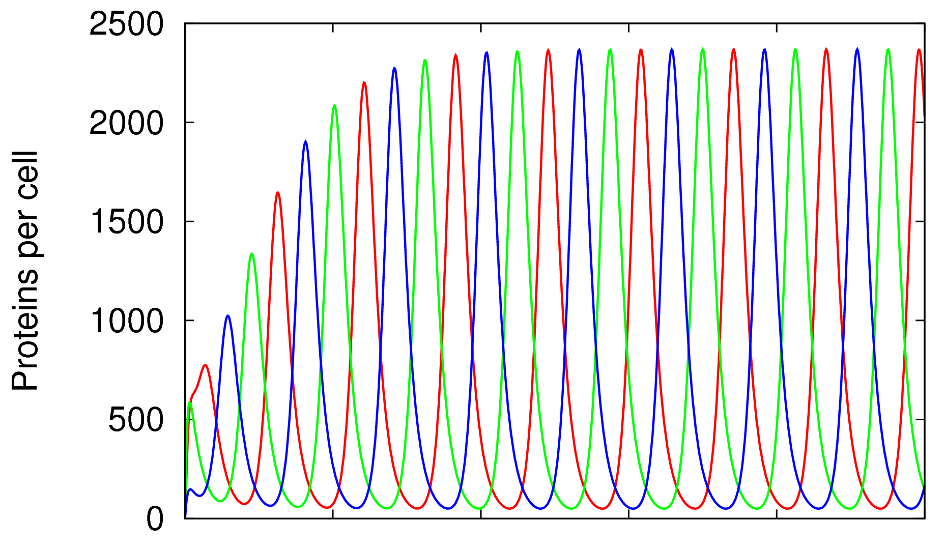
\includegraphics[width=0.6\textwidth]{images/simEx1.png}
\caption{Time-course simulation of the repressilator model, imported from BioModels Database and simulated in COPASI. The number of repressor proteins lacI, tetR and cI is shown. (taken from \cite{Waltemath:2011})}
\label{fig:simEx1}
\end{figure}

\subsection{Applying pre-processing}
\label{sec:examplePreprocessing}
The fine-tuning of the model can be shown by adjusting parameters before simulation. When changing the initial values of the parameters \emph{protein copies per promoter} and \emph{leakiness in protein copies per promoter} the system's behavior switches from sustained oscillation to asymptotic steady-state. The adjustments leading to that behavior may be described as: 

\begin{enumerate}
\item{Import the model as above.}
\item{Change the value of the parameter \code{tps$\_$repr} from “0.0005” to “1.3e-05”. }
\item{Change the value of the parameter \code{tps$\_$active} from “0.5 “ to “ 0.013“.}
\item{Select a deterministic method.}
\item{Run a uniform time course for the duration of 1000~min with an output interval of 1~min.}
\item Plot the amount of lacI, tetR and cI against time in a 2D Plot.
\end{enumerate}

\fig{simEx3} shows the result of the simulation.
%
\begin{figure}
\centering
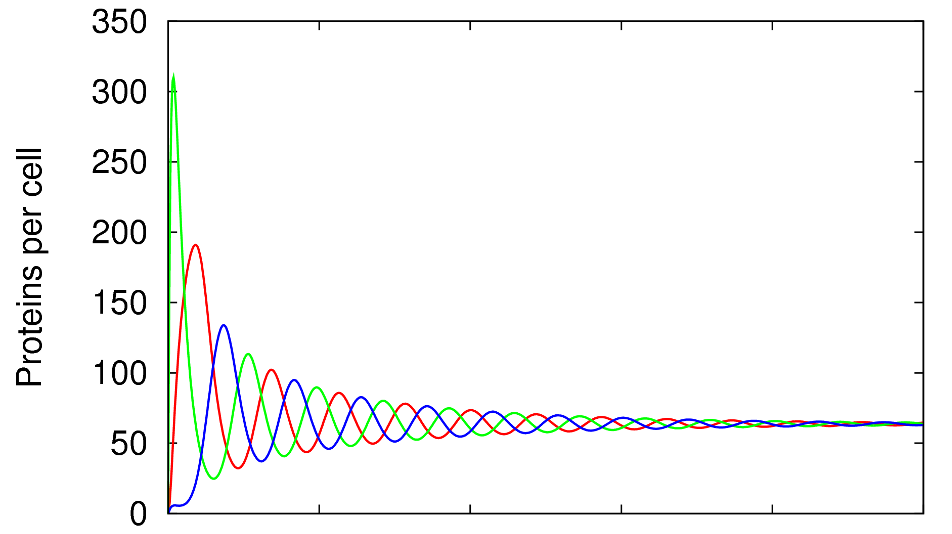
\includegraphics[width=0.7\textwidth]{images/simEx3.png}
\caption{Time-course simulation of the repressilator model, imported from BioModels Database and simulated in COPASI after modification of the initial values of the \emph{protein copies per promoter} and the \emph{leakiness in protein copies per promoter}. The number of repressor proteins lacI, tetR and cI is shown. (taken from \cite{Waltemath:2011})}
\label{fig:simEx3}
\end{figure}


\subsection{Applying post-processing}
The raw numerical output of the simulation steps may be subjected to data post-processing before plotting or reporting.  In order to describe the production of a normalized plot of the time-course in the first example (section \ref{sec:intro1}), depicting the influence of one variable on another (in phase-planes), one could define the following further steps:

(Please note that the description steps 1 - 4 remain as given in section \ref{sec:intro1} above.)
\begin{enumerate}
\item[5.]{Collect lacI(t) , tetR(t) and cI(t).}
\item[6.]{Compute the highest value for each of the repressor proteins,  max(lacI(t)), max(tetR(t)), max(cI(t)).}
\item[7.]{Normalize the data for each of the repressor proteins by dividing each time point by the maximum value, i.\,e.\ lacI(t)/max(lacI(t) ), tetR(t)/max(tetR(t)) , and cI(t)/max(cI(t)).}
\item[8.]{Plot the normalized \code{lacI} protein as a function of the normalized \code{cI}, the normalized \code{cI}  as a function of the normalized \code{tetR} protein, and the normalized \code{tetR} protein against the normalized \code{lacI} protein in a 2D plot.}
\end{enumerate}
\fig{simEx2} illustrates the result of the simulation after post-processing of the output data. 
\begin{figure}
\centering
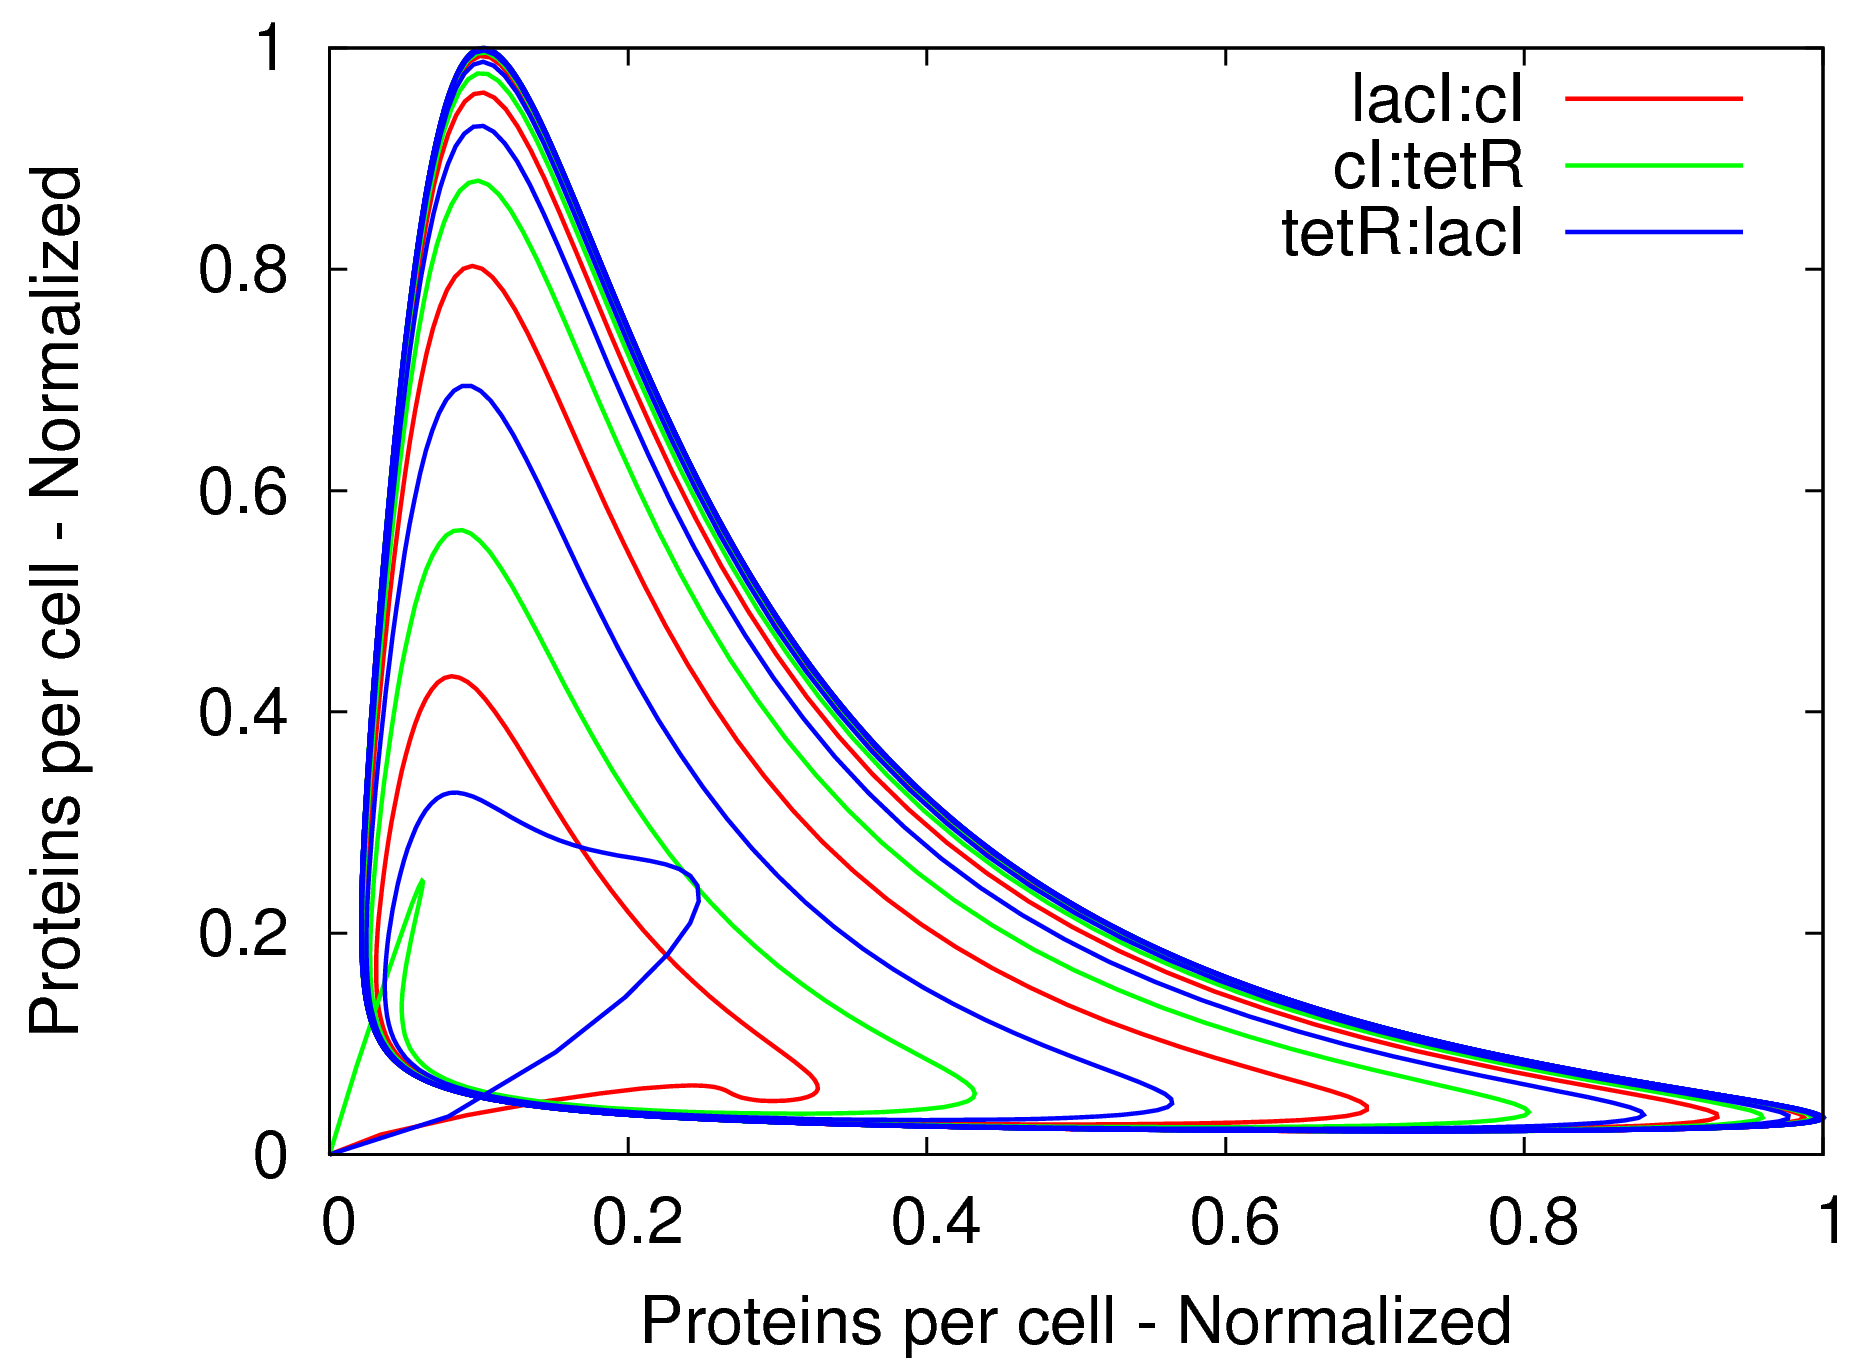
\includegraphics[width=0.7\textwidth]{images/simEx2.png}
\caption{Time-course simulation of the repressilator model, imported from BioModels Database and simulated in COPASI, showing the normalized temporal evolution of repressor proteins lacI, tetR and cI in phase-plane. (taken from \cite{Waltemath:2011})}
\label{fig:simEx2}
\end{figure}


%%% Local Variables: 
%%% mode: latex
%%% TeX-master: "../sed-ml-L1V3"
%%% End: 


% ~~~~~~~~~~~~~~~~~~~~~~~~~~~~~~~~~~~~
%% OVERVIEW  (BPMN)
% ~~~~~~~~~~~~~~~~~~~~~~~~~~~~~~~~~~~~
\chapter{Overview of SED-ML}
\label{sec:overview}
% overview
The \emph{Simulation Experiment Description Markup Language} (SED-ML) is an XML-based format for the description of simulation experiments. It serves to store information about the simulation experiment performed on one or more models with a given set of outputs. Support for SED-ML compliant simulation descriptions will enable the exchange of simulation experiments across tools.
\section{Conventions}
%
The Business Process Modeling Notation Version 1.2 (BPMN) was initially intended to describe internal business procedures (processes) in a graphical way. However, we will use BPMN to graphically describe the steps and processes of setting up a simulation experiment description. The major parts of BPMN that are used to specify SED-ML are activities, gateways, events, data, and documentation. 

An \emph{activity} is ``work that is performed on a [..] process'', for example ``Specify the simulation settings''. Activities may be atomic or non-atomic. SED-ML in particular makes use of the \emph{task} activities, \ie specific work units that need to be performed. Non-atomic tasks might be collapsed or expanded in the graphical representation (\fig{task}). Each collapsed subprocess has a corresponding expanded subprocess definition.

\begin{figure}[h]
\centering
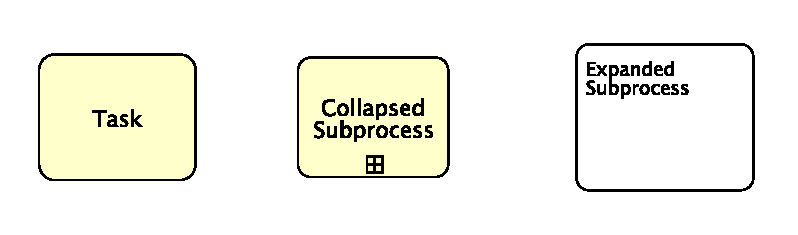
\includegraphics[width=0.5\textwidth]{images/processes.pdf}
\caption{BPMN activities: task, collapsed process, expanded subprocess}
\label{fig:task}
\end{figure}

\emph{Gateways} serve as means to control the flow of sequence in the diagram. As the term already implies, a gateway needs some ``mechanism that either allows or disallows passage through'' \citep{White:2004}. The result of a gateway pass-through can be that processes are merged or split. Graphically, a gateway is represented as a diamond. 

\begin{figure}[h]
\centering
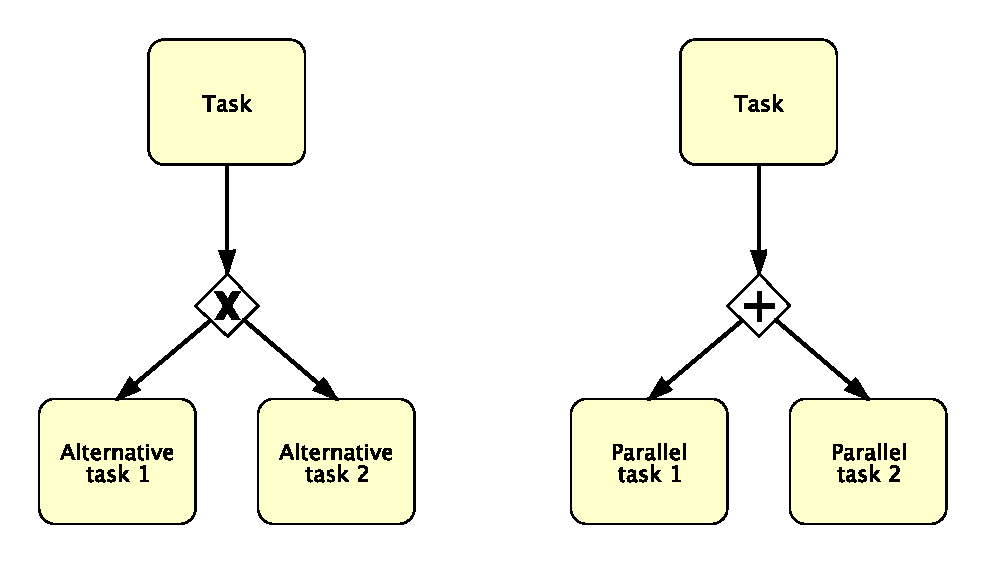
\includegraphics[width=0.5\textwidth]{images/gateways.pdf}
\caption{BPML gateway types: Exclusive (left), parallel (right)}
\label{fig:gateways}
\end{figure}

While there exist a number of different gateway types \citep[p.~93]{White:2004}, the SED-ML specification only uses the parallel and the exclusive gates  (\fig{gateways}). 

\emph{Exclusive} gateways -- also denoted as decisions -- allow the sequence flow to take two or more alternative paths (\fig{gateways}, left hand side). However, \emph{only one} of the paths may be chosen (not more). Sometimes two alternative branches need to be merged together again, in which case the exclusive gate must be used as well: The sequence flow continues as soon as \emph{one} of the incoming processes send a signal. An exclusive gateways is marked by an \code{X} in the graphical notation.

\emph{Parallel} gateways, ``provide a mechanism to synchronize parallel flow and to create parallel flow'' \citep{White:2004} (\fig{gateways}, right hand side). They are used to show parallel paths in the workflow; even if sometimes not required they might help in understanding the process. Synchronisation allows to start two processes in parallel at the same time in the sequence flow: The sequence flow will continue with \emph{all} processes leaving the parallel gateway. Joining two processes with a parallel gateway is also possible: the process flow will only continue after a signal has arrived from \emph{all} processes coming in the parallel gateway. A parallel gateway is marked by a \code{+} in the graphical notation.

\emph{Events} mark everything happening during the execution of the sequence flow, usually they interrrupt the business process, having some cause or impact on the execution. From the broad range of events that BPMN offers, SED-ML only uses a small subset, namely the start event and the end event (\fig{connectorEvents}).

\begin{figure}[h]
\centering
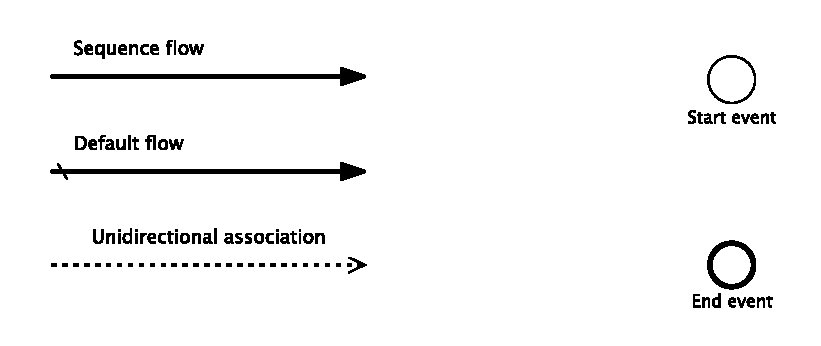
\includegraphics[width=0.5\textwidth]{images/connectors.pdf}
\caption{BPML connectors (left) and events (right).}
\label{fig:connectorEvents}
\end{figure}

All events are graphically drawn as small circles. A \emph{start event} is drawn with a single thin line and mark the start of a process, it can not have any incoming sequence flow. Start events may be triggered by different mechanisms, for the case of SED-ML the untyped start event (no marker inside the circle) is used. The trigger to start the process is ``Create new simulation experiment''. The \emph{end event} is marked with a thick line. It indicates the end of a process. SED-ML specification makes use of the untyped end event (no marker inside the circle). The end event is used to show the end of sub-processes as well as processes. If the end of a sub-process is reached, the sequence flow returns to the according parent process.

\emph{Connectors} are used to combine different BPMN objects with each other (\citet[p.~30]{White:2004} show the full list of valid connections). SED-ML uses only a subset of available connectors, namely sequence flow, default flow, and unidirectional associations (\fig{connectorEvents}). \emph{Sequence flow} defines the execution order of activities. \emph{Default flow} marks the default branch to be chosen if other conditions leave various possibilities for further execution of the sequence flow. A \emph{unidirectional association} is used to indicate that a data object is modified, i.\,e. read and written during the execution of an activity \citep{bpmnPoster}.

%
The rough SED-ML workflow is shown in Figure \ref{fig:sedmlWorkflow}.
%
\begin{figure}[h]
\centering
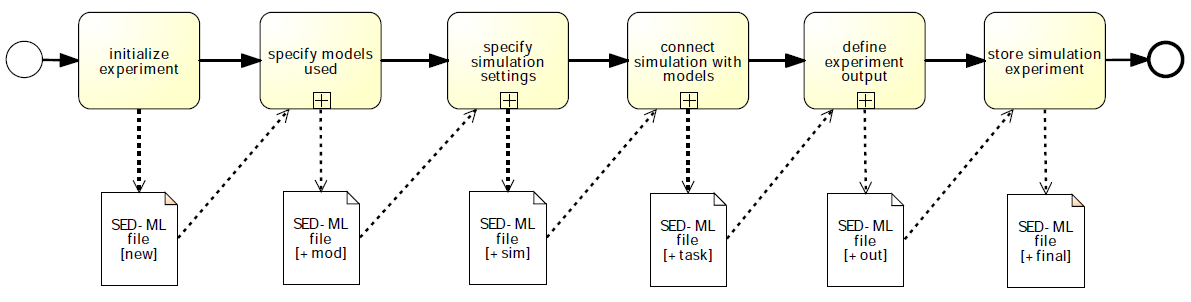
\includegraphics[width=\textwidth]{images/bpmn/sedMainOryx.png}
\caption{The process of defining a simulation experiment in SED-ML (overview)}
\label{fig:sedmlWorkflow}
\end{figure}
%
The process of defining a SED-ML simulation experiment starts by initialising the experiment and creating a new SED-ML file. Afterwards, the \concept{models} needed for the simulation are specified and stored into the existing SED-ML file (Section~\ref{overview:models}). In a third step, the simulation experiment \concept{setups} are defined and stored into the same file (Section~\ref{overview:simulation}). To assign a setup to a number of models used in the experiment, these connections have to be defined and recorded (Section~\ref{overview:task}), called \concept{task} in SED-ML. After simulation, the \concept{output} should be defined, based on the specified tasks and performed simulation experiment. The information is added to the existing SED-ML file (Section~\ref{overview:output}). In the end, the whole experiment is stored in the final SED-ML file.
%
All collapsed processes are described in the following sections. Examples in XML are provided in the more technical description.

\section{Models}
\label{overview:models}
To define a simulation experiment, first of all a new SED-ML file is created. The models to be used in the experiment (zero or many) are referenced, using a link to a model description in some open, curated model database (e.\,g.\ Biomodels Database \citep{LDR+10} or CellML Repository \citep{BBC+09}). All necessary changes to correctly simulate the model are defined, e.\,g., assigning new parameter values or updating the mathematics of the model (Figure~\ref{fig:workflowModel}).
%
\begin{figure}[h]
\centering
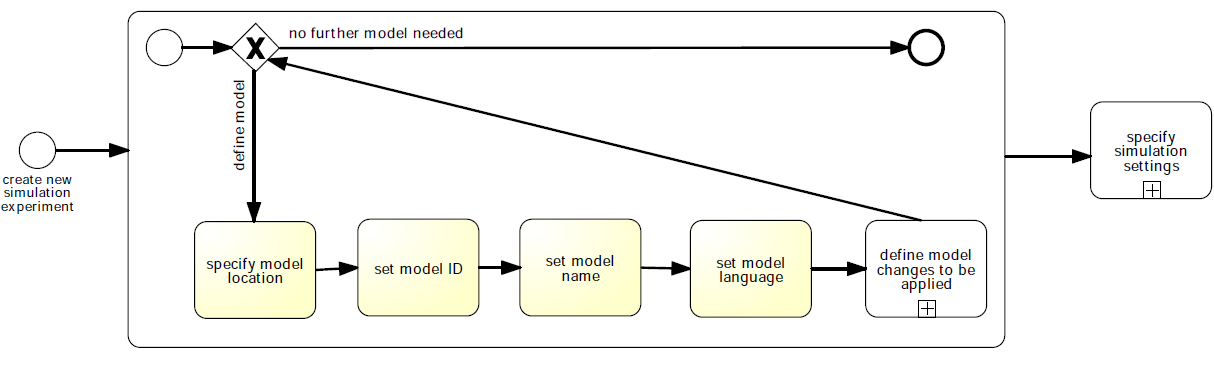
\includegraphics[width=0.8\textwidth]{images/bpmn/sedModelOryx.png}
\caption{The process of defining model(s) in SED-ML}
\label{fig:workflowModel}
\end{figure}
%
The procedure is repeated until all models participating in the experiment have been described. Each such model gets an internal SED-ML ID and an optional name.

\section{Simulation setup}
\label{overview:simulation}
Secondly, the simulation setups (zero or many) used throughout the simulation experiment are described (Figure \ref{fig:workflowSimulation}). 
%
%
\begin{figure}[h]
\centering
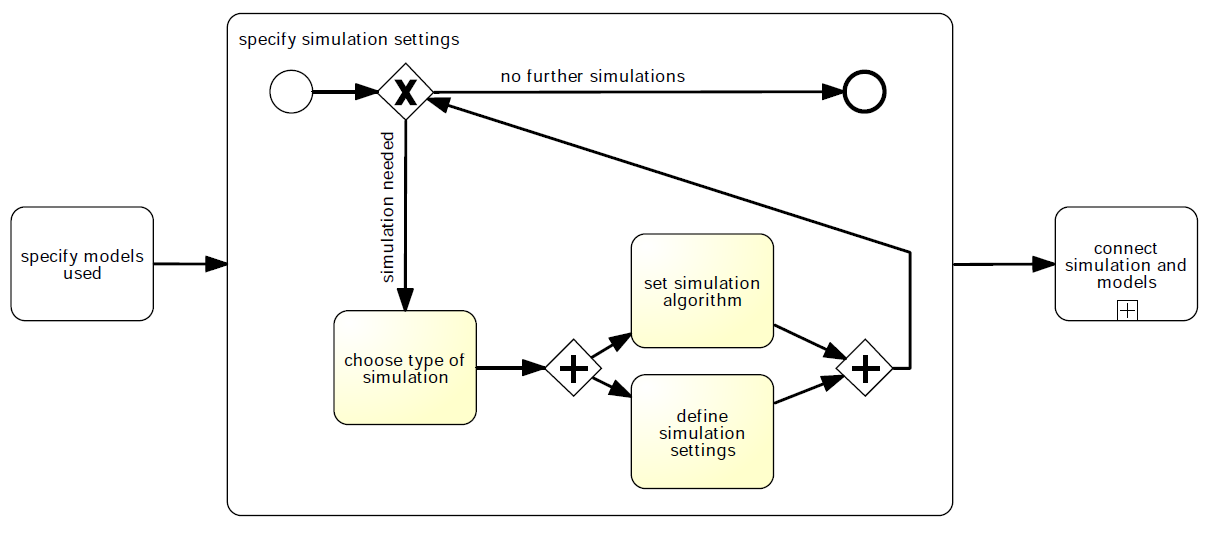
\includegraphics[width=0.8\textwidth]{images/bpmn/sedSimulationOryx.png}
\caption{The process of defining simulation(s) in SED-ML}
\label{fig:workflowSimulation}
\end{figure}
%
Those may stem from various different types of simulation, e.\,g., steady state analysis or bifurcation.  Depending on the specific type of experiment, the information encoded for the simulation setup might differ. Thus, the definition of simulation settings is specific to the simulation experiment.

In a simple case the experiment consists of one simulation, but it can get far more complex. For example, one might define a nested sequence of simulations, in which case every simulation has to be defined separately.
Each simulation setup gets its own internal ID and an optional name. For each of the setups, the simulation algorithm to be used for that simulation is defined through a reference to a well-defined algorithm name, e.\,g. an ontology or controlled vocabulary. One approach to define such a controlled vocabulary of simulation algorihtms is the \emph{Kinetic Simulation Algorithm Ontology} (Section~\ref{sec:kisao}). 
%
The setup definition is repeated until all different simulations have been described.

\section{Task}
\label{overview:task}
SED-ML allows to apply one defined simulation setting to one defined model at a time. However, any number of \concept{tasks} may be defined inside a simulation experiment description (Figure \ref{fig:workflowTask}). 
%
\begin{figure}[h]
\centering
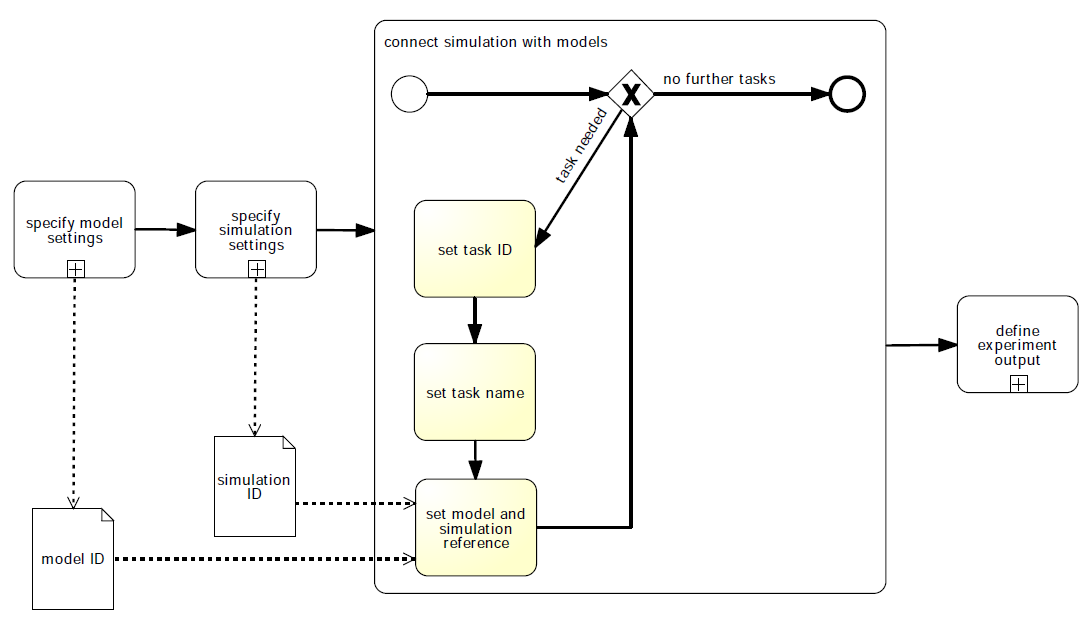
\includegraphics[width=0.7\textwidth]{images/bpmn/sedTaskOryx.png}
\caption{The process of defining simulation task(s) in SED-ML}
\label{fig:workflowTask}
\end{figure}
%
To do so, each task refers to one of the formerly specified models and to one of the formerly specified simulation setups. Each task has its own ID and an optional name. The process of task definition is repeated until all tasks have been defined.


\section{Output}
\label{overview:output}
The SED-ML finally consists of output definitions that describe what kind of output the experiment uses to present the simulation result to the user, i.\,e., a plot or a data table (Figure \ref{fig:workflowOutput}), and also which data is part of the output. 
%
\begin{figure}[h]
\centering
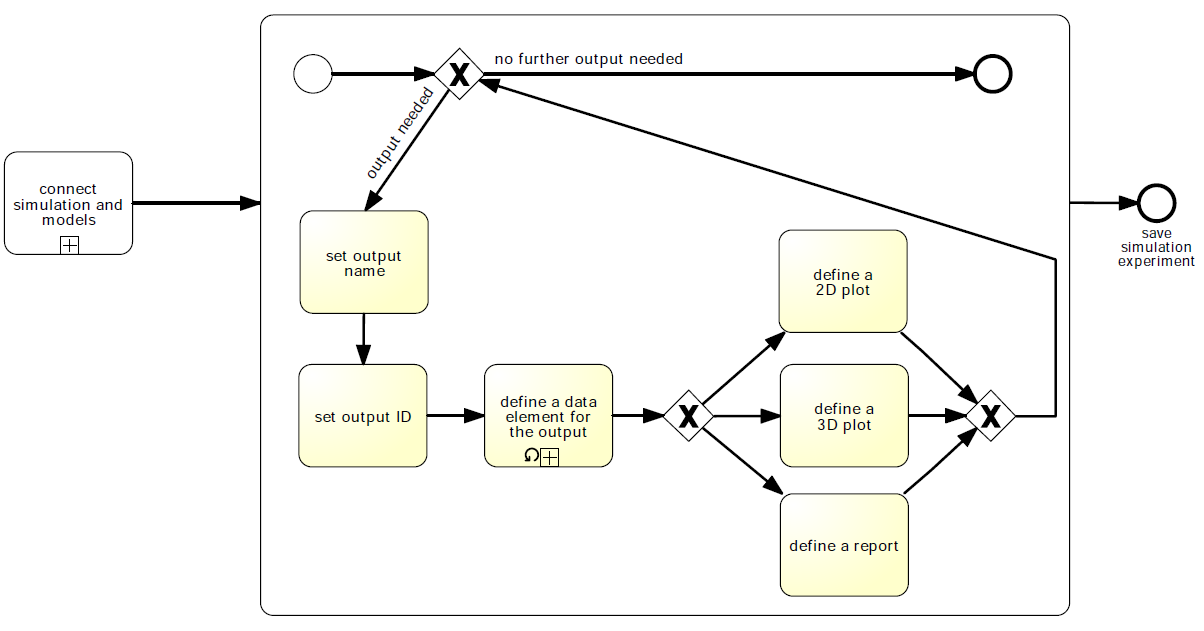
\includegraphics[width=0.7\textwidth]{images/bpmn/sedOutputOryx.png}
\caption{The process of defining output(s) in SED-ML}
\label{fig:workflowOutput}
\end{figure}
%
Therefore, SED-ML first defines a set of \concept{data generators} (Figure \ref{fig:workflowDataGenerator}), which are then used to specify a particular result, i.\,e. output (Section~\ref{overview:dataGen}). 

The SED-ML specification comes with three pre-defined types of outputs: 2D- and 3D plots, and reports. All use the aforementioned data generators to specify the information to be plotted on the different axes, or in the table comlumns respectively.
\section{Data Generator}
\label{overview:dataGen}
%
\begin{figure}[h]
\centering
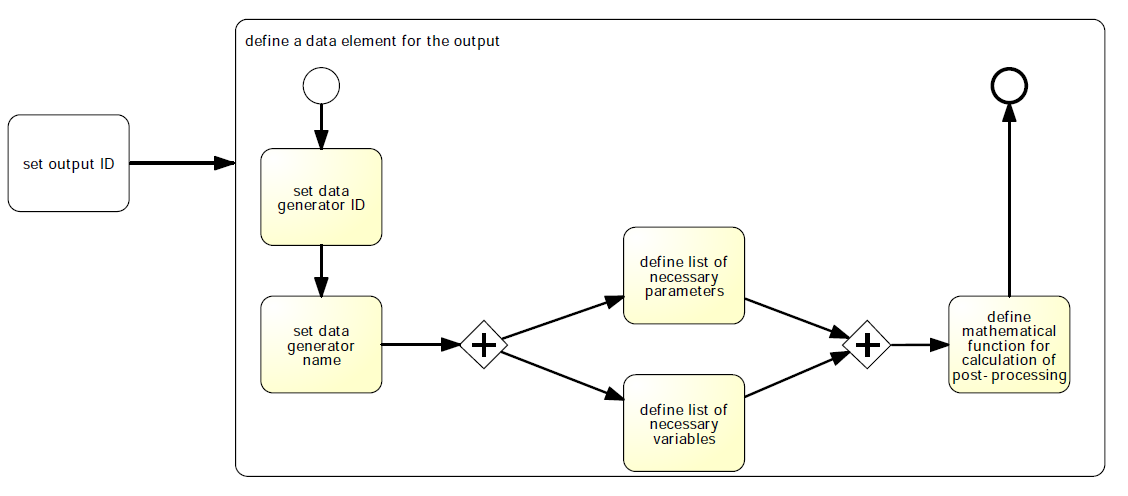
\includegraphics[width=0.7\textwidth]{images/bpmn/sedDataGeneratorOryx.png}
\caption{The process of defining data generator(s) in SED-ML}
\label{fig:workflowDataGenerator}
\end{figure}
%
A data generator may use data elements, e.\,g., variables or parameters, that either (1) have been taken directly from the model, or (2) have been generated in a post-processing step. If post-processing needs to be applied, variables and parameters from the various, previously defined models may be used, but also existing global parameters, such as \emph{time}.
If the variables are taken from existing models, a reference to the model and the particular variable needs to be given. 
If post-processing is necessary, a reference to an existing variable or parameter, including other data generators, has to be provided. Additional mathematical rules to be applied on the referred variable or parameter must then  be specified. 
%
In a SED-ML file, any number of data generators can be created for later re-use in the output definition.



%%% Local Variables: 
%%% mode: latex
%%% TeX-master: "../sed-ml-L1V2"
%%% End: 



%%% Local Variables: 
%%% mode: latex
%%% TeX-master: "../sed-ml-L1V2"
%%% End: 


  %% EXAMPLE OF A SIMULATION EXPERIMENT DESCRIPTION (INFORMAL)
  % motivation
\section{Motivation: A sample experiment}
\label{motivation:example}

The \emph{repressilator} is a rather small, though famous, model that is capable of displaying rich and variable behaviors. 
We will use this model to demonstrate how a simulation experiment can be described simply and effectively. 
The simulation example is taken from \citet{Waltemath:2011}. 

The \emph{repressilator} is a synthetic oscillating network of transcription regulators in Escherichia coli \citep{Elowitz:2000}. The network is composed of the three repressor genes Lactose Operon Repressor (lacI), Tetracycline Repressor (tetR) and Repressor CI (cI), which code for proteins binding to the promoter of the other, blocking their transcription. The three inhibitions together in tandem, form a cyclic negative-feedback loop. To describe the interactions of the molecular species involved in the network, the authors built a simple mathematical model of coupled first-order differential equations. All six molecular species included in the network (three mRNAs, three repressor proteins) participated in creation (transcription/translation) and degradation processes. The model was used to determine the influence of the various parameters on the dynamic behavior of the system. In particular, parameter values were sought which induce stable oscillations in the concentrations of the system components. Oscillations in the levels of the three repressor proteins are obtained by numerical integration. 

\subsection{A simple time-course simulation}
 \label{sec:intro1}
 The first experiment we intend to run on the model is the simulation that will lead to the oscillation shown in Figure 1c of the reference publication \citep{Elowitz:2000}. This simulation experiment can be described as:

\begin{enumerate}
 	\item{Import the model identified by the Unified Resource Identifier (URI) \citep{Berners-Lee:2005} \url{urn:miriam:biomodels.db:BIOMD0000000012}.}
 	\item {Select a deterministic method.}
 	\item{Run a uniform time course simulation for 1000~min with an output interval of 1~min.}
 	\item{Plot the amount of \code{lacI}, \code{tetR} and \code{cI} against time in a 2D Plot.}
 \end{enumerate}

Following those steps and performing the simulation in the simulation tool COPASI \citep{Hoops:2006} led to the result shown in \fig{simEx1}. 

\begin{figure}
\centering
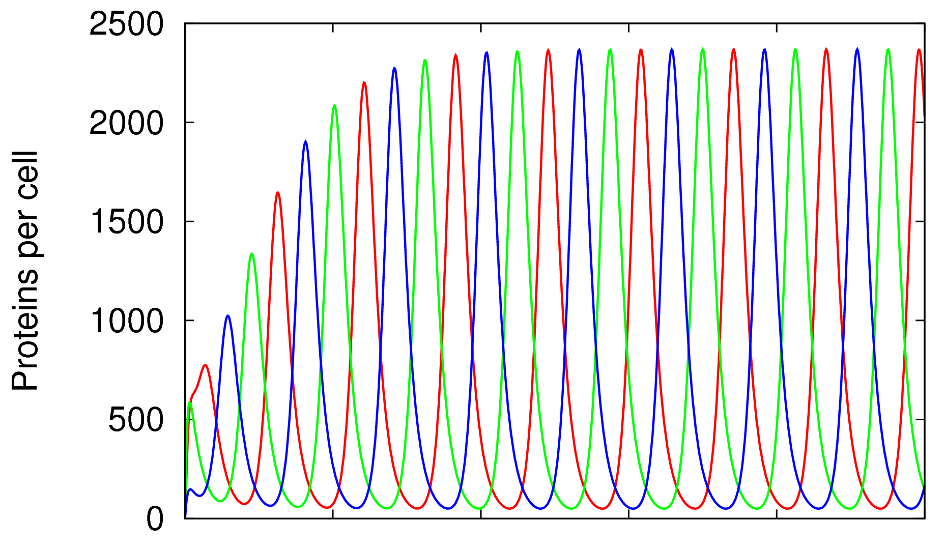
\includegraphics[width=0.6\textwidth]{images/simEx1.png}
\caption{Time-course simulation of the repressilator model, imported from BioModels Database and simulated in COPASI. The number of repressor proteins lacI, tetR and cI is shown. (taken from \cite{Waltemath:2011})}
\label{fig:simEx1}
\end{figure}

\subsection{Applying pre-processing}
\label{sec:examplePreprocessing}
The fine-tuning of the model can be shown by adjusting parameters before simulation. When changing the initial values of the parameters \emph{protein copies per promoter} and \emph{leakiness in protein copies per promoter} the system's behavior switches from sustained oscillation to asymptotic steady-state. The adjustments leading to that behavior may be described as: 

\begin{enumerate}
\item{Import the model as above.}
\item{Change the value of the parameter \code{tps$\_$repr} from “0.0005” to “1.3e-05”. }
\item{Change the value of the parameter \code{tps$\_$active} from “0.5 “ to “ 0.013“.}
\item{Select a deterministic method.}
\item{Run a uniform time course for the duration of 1000~min with an output interval of 1~min.}
\item Plot the amount of lacI, tetR and cI against time in a 2D Plot.
\end{enumerate}

\fig{simEx3} shows the result of the simulation.
%
\begin{figure}
\centering
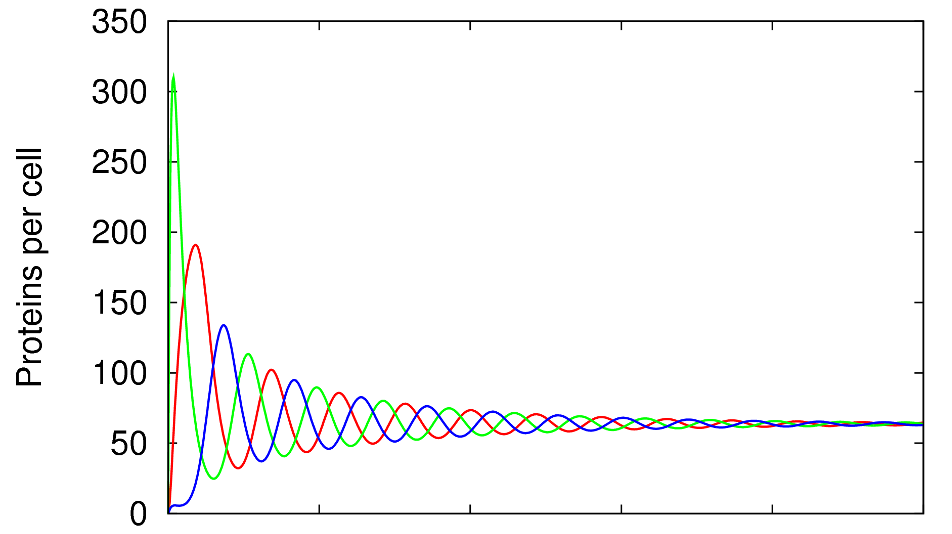
\includegraphics[width=0.7\textwidth]{images/simEx3.png}
\caption{Time-course simulation of the repressilator model, imported from BioModels Database and simulated in COPASI after modification of the initial values of the \emph{protein copies per promoter} and the \emph{leakiness in protein copies per promoter}. The number of repressor proteins lacI, tetR and cI is shown. (taken from \cite{Waltemath:2011})}
\label{fig:simEx3}
\end{figure}


\subsection{Applying post-processing}
The raw numerical output of the simulation steps may be subjected to data post-processing before plotting or reporting.  In order to describe the production of a normalized plot of the time-course in the first example (section \ref{sec:intro1}), depicting the influence of one variable on another (in phase-planes), one could define the following further steps:

(Please note that the description steps 1 - 4 remain as given in section \ref{sec:intro1} above.)
\begin{enumerate}
\item[5.]{Collect lacI(t) , tetR(t) and cI(t).}
\item[6.]{Compute the highest value for each of the repressor proteins,  max(lacI(t)), max(tetR(t)), max(cI(t)).}
\item[7.]{Normalize the data for each of the repressor proteins by dividing each time point by the maximum value, i.\,e.\ lacI(t)/max(lacI(t) ), tetR(t)/max(tetR(t)) , and cI(t)/max(cI(t)).}
\item[8.]{Plot the normalized \code{lacI} protein as a function of the normalized \code{cI}, the normalized \code{cI}  as a function of the normalized \code{tetR} protein, and the normalized \code{tetR} protein against the normalized \code{lacI} protein in a 2D plot.}
\end{enumerate}
\fig{simEx2} illustrates the result of the simulation after post-processing of the output data. 
\begin{figure}
\centering
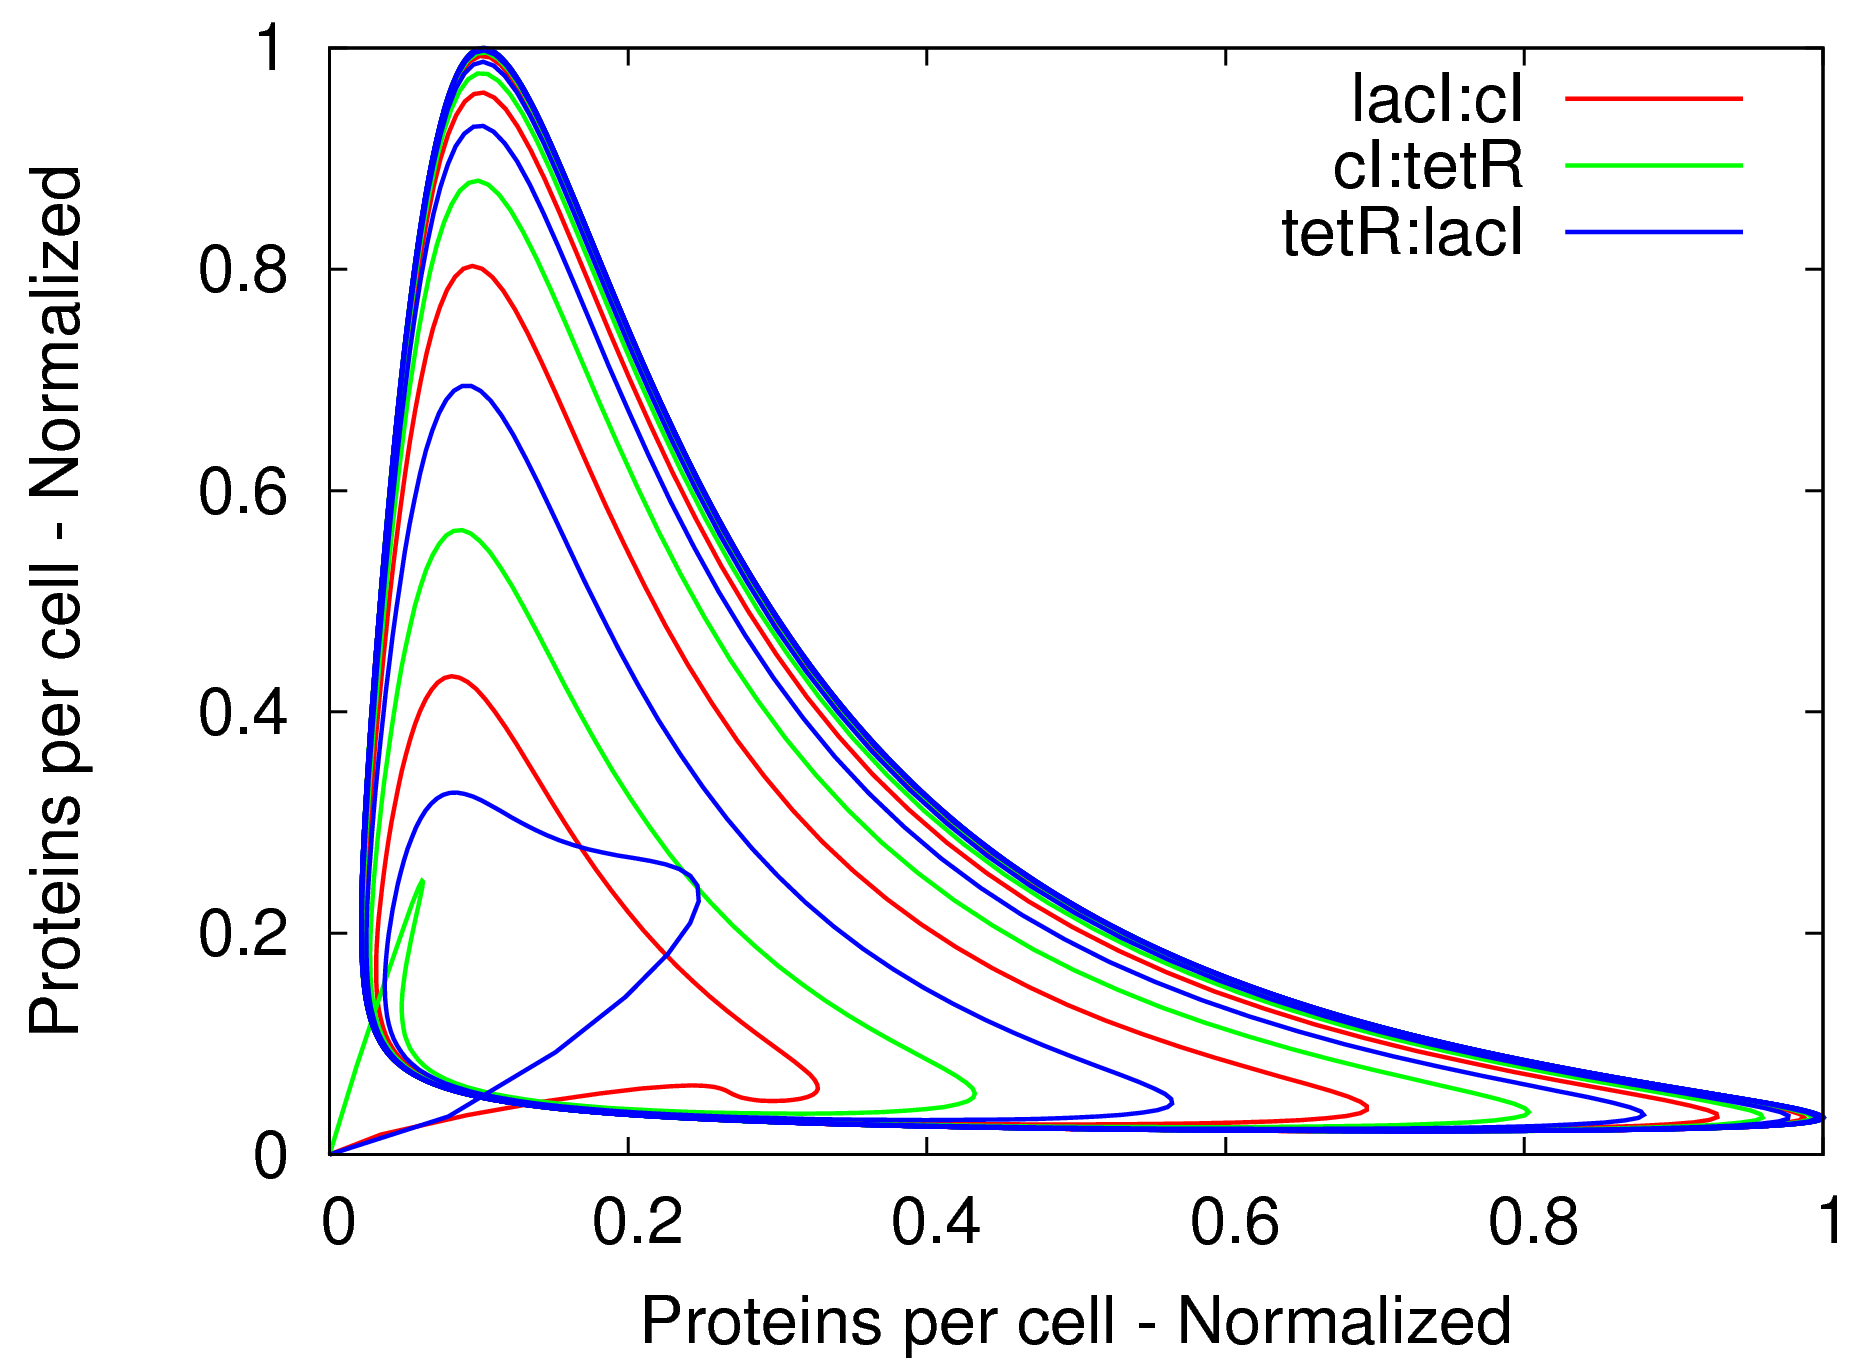
\includegraphics[width=0.7\textwidth]{images/simEx2.png}
\caption{Time-course simulation of the repressilator model, imported from BioModels Database and simulated in COPASI, showing the normalized temporal evolution of repressor proteins lacI, tetR and cI in phase-plane. (taken from \cite{Waltemath:2011})}
\label{fig:simEx2}
\end{figure}


%%% Local Variables: 
%%% mode: latex
%%% TeX-master: "../sed-ml-L1V3"
%%% End: 


  %% NOTATION CONVENTIONS
  \section{Conventions used in this document}
\label{sec:conventions}


%% UML
\subsection{UML Classes}
\label{sec:umlconventions}
A SED-ML UML class (\fig{umlClass}) consists of a class name (\code{ClassName}) and a number of attributes (\code{attribute}) each of a specific data type (\code{type}). The SED-ML UML specification does not make use of UML \code{operations}.
\begin{figure}[h]
\centering
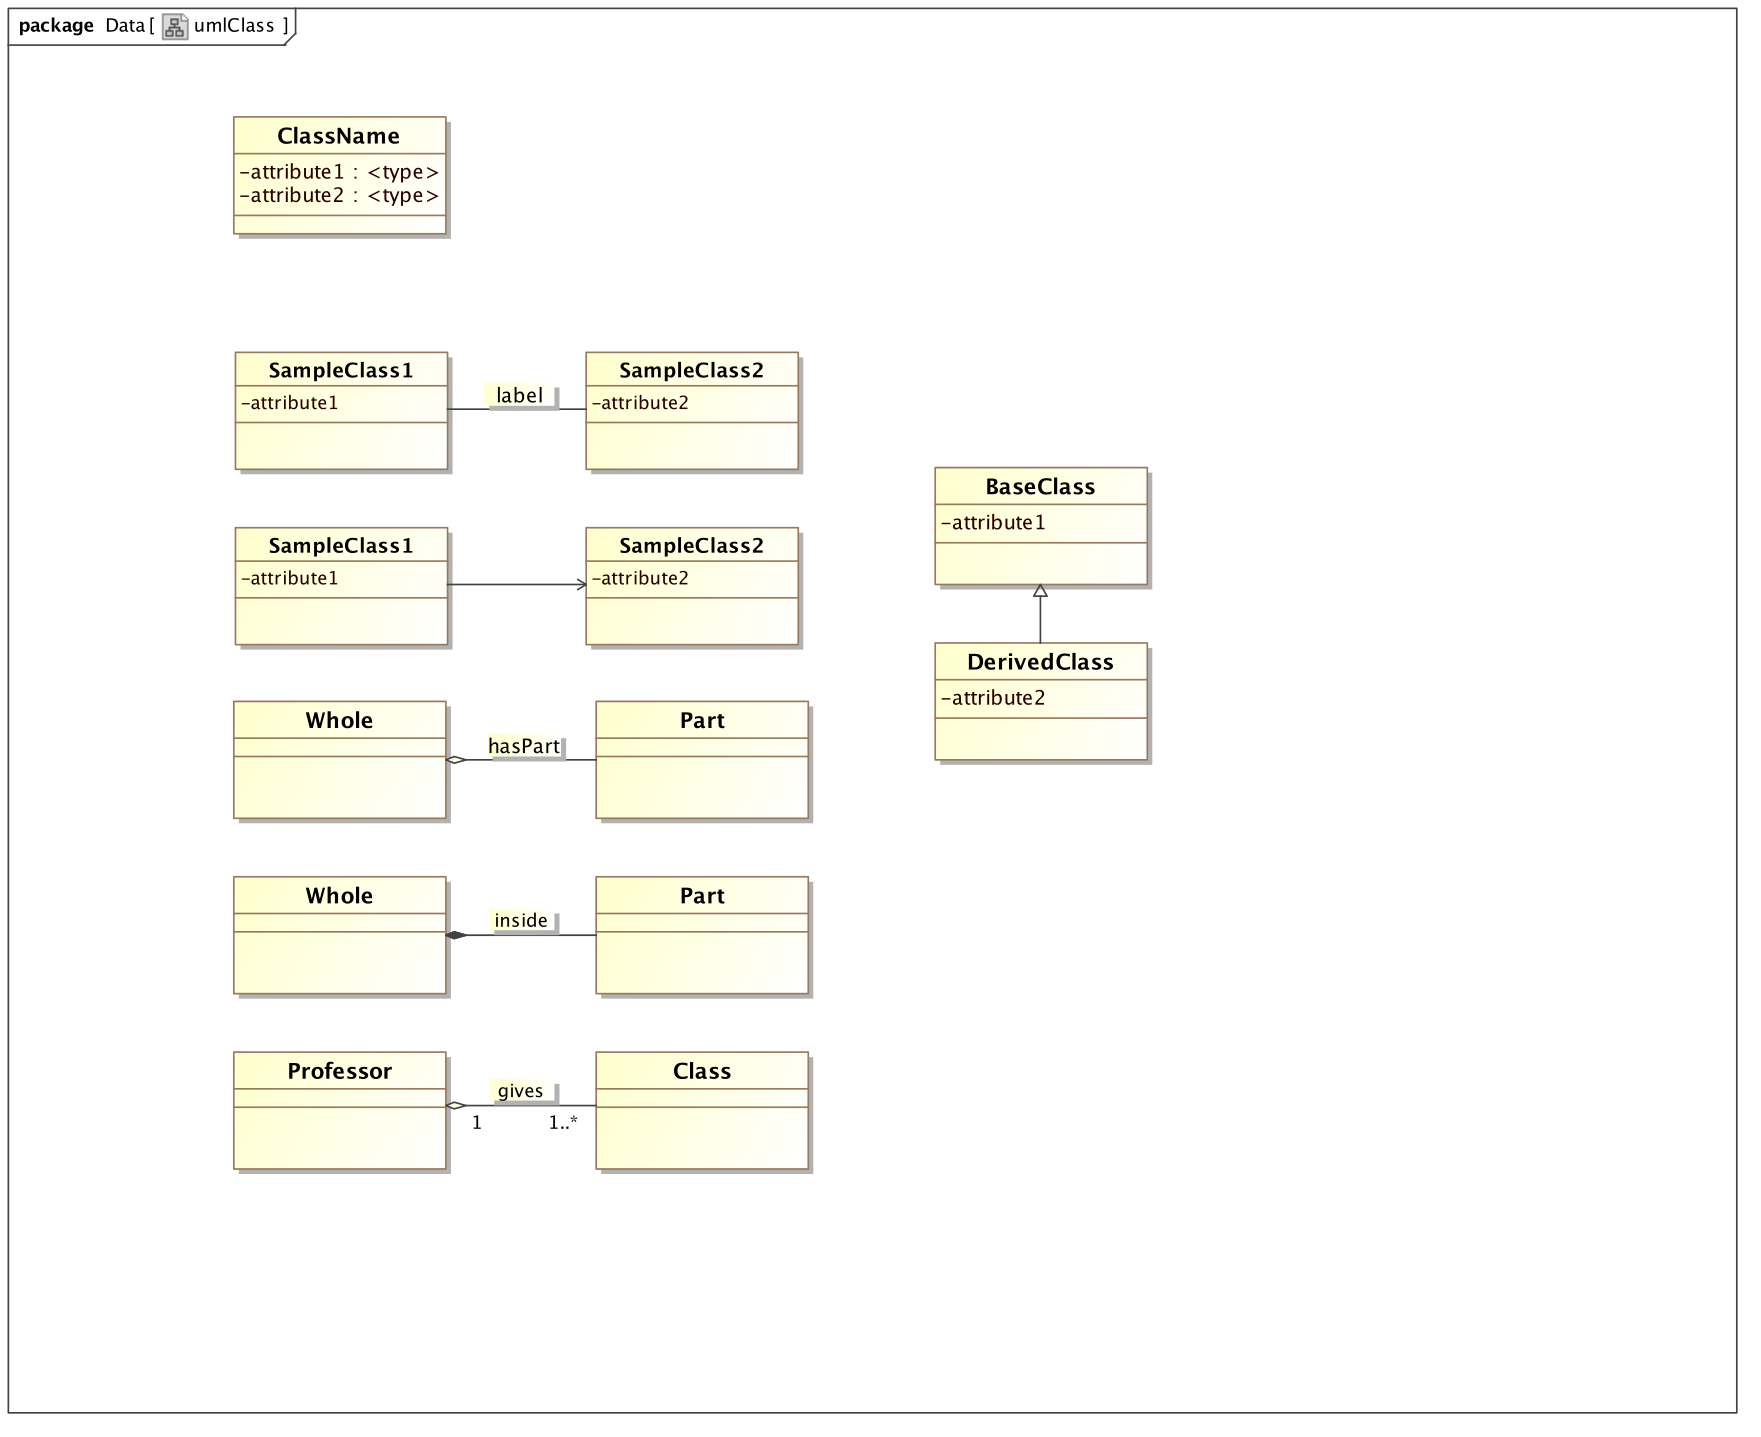
\includegraphics[width=0.2\textwidth]{images/pdf/umlClass}
\caption{SED-ML UML class with class names and attributes}
\label{fig:umlClass}
\end{figure}

SED-ML class names always begin with upper case letters. If they are composed of different words, the camel case style is used, as in e.\,g.\ \code{DataGenerator}.

\subsection{UML Relationships}
%% RELATIONS
\subsubsection{UML Relation Types}
\begin{figure}[h]
\centering
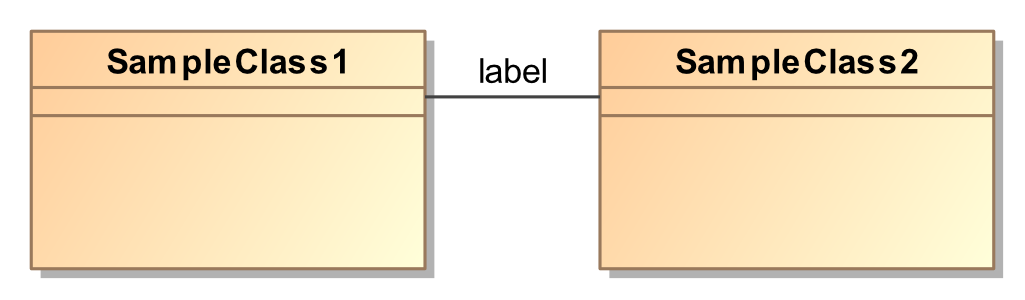
\includegraphics[width=0.5\textwidth]{images/pdf/classRelation}
\caption{UML Class connectors}
\label{fig:umlConnectors}
\end{figure}

Links between classes specify the connection of objects with each other (\fig{umlConnectors}). The different relation types used in the SED-ML specification include aggregation, composite aggregation, and generalisation. The label on the line is called symbol (\code{label}) and describes the relation of the objects of both classes. 

%% Association
The \concept{association} (\fig{umlAssociation}) indicates the existence of a connection between the objects of the participating classes. Often associations are directed to show how the label should be read (in which direction). Associations can be uni-directional (one arrowhead), or bidirectional (zero or two arrowheads).  
\begin{figure}[h]
\centering
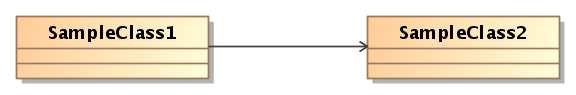
\includegraphics[width=0.5\textwidth]{images/pdf/umlAssociation}
\caption{UML Association}
\label{fig:umlAssociation}
\end{figure}

 
%% Aggregation
The \concept{aggregation} (\fig{umlAggregation}, top) indicates that the objects of the participating classes are connected in a way that one class (\code{Whole}) consists of several parts (\code{Part}). In an aggregation, the parts may be independent of the whole. For example, a car (\code{Whole})  has several parts called wheel (\code{Part}); however, the wheels can exist independently of the car while the car requires the wheels in order to function.
\begin{figure}[h]
\centering
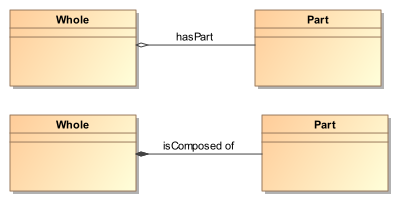
\includegraphics[width=0.5\textwidth]{images/pdf/umlAggregation}
\caption{UML Aggregation (top) and Composition (bottom)}
\label{fig:umlAggregation}
\end{figure}

%% Composite Aggregation
The \concept{composite aggregation} (\fig{umlAggregation}, bottom) indicates that the objects of the participating classes are connected in a way that one class (\code{Whole}) consists of several parts (\code{Part}). In contrast to the aggregation, the subelements (\code{Part}) are dependent on the parent class (\code{Whole}). An example is that a university (\code{Whole}) consists of a number of departments (\code{Part}) which have a so-called ``lifetime responsibility'' with the university, e.\,g.\ if the university vanishes,  the departments will vanish with it \citep{Bel03}.

%% Inheritance
The \concept{generalisation} (\fig{umlGeneralisation}) allows to extend classes (\code{BaseClass}) by additional properties. The derived class (\code{DerivedClass}) inherits all properties of the base class and defines additional ones. In the given example, an instance of \code{DerivedClass} has two attributes \code{attribute1} and \code{attribute2}.
%
\begin{figure}[h]
\centering
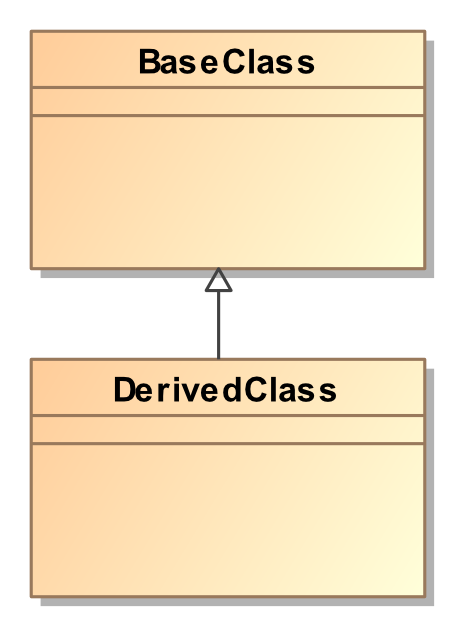
\includegraphics[width=0.2\textwidth]{images/pdf/umlGeneralisation}
\caption{UML Generalisation}
\label{fig:umlGeneralisation}
\end{figure}
%
%% CARDINALITIES
\subsubsection{UML multiplicity}
UML multiplicity defines the number of objects in one class that can be related to one object in the other class (also known as \concept{cardinality}). Possible types of multiplicity include values (1), ranges (1$..$4), intervals (1,3,9), or combinations of ranges and intervals. The standard notation for ``many'' is the asterisk (*). 

Multiplicity can be defined for both sides of a relationship between classes. The default relationship is ``many to many''. 
The example in \fig{umlMulti} expresses that a class is given by a professor, and a professor might give one to many classes.
\begin{figure}[h]
\centering
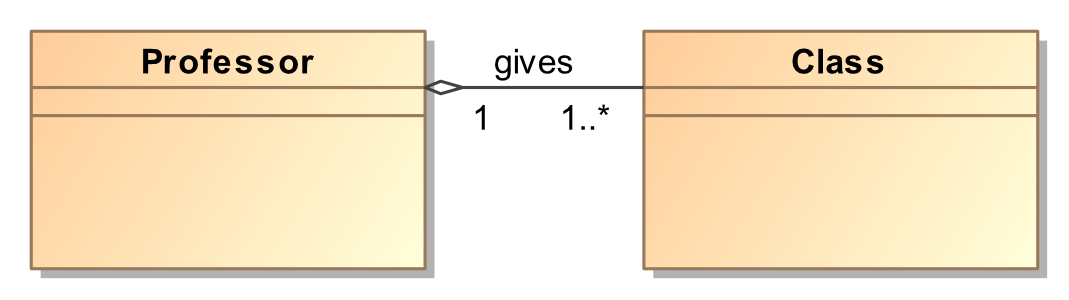
\includegraphics[width=0.4\textwidth]{images/pdf/umlMultiplicity}
\caption{UML Multiplicity in an Aggregation}
\label{fig:umlMulti}
\end{figure}

%% XML SCHEMA
\subsection{XML Schema language elements}
The main building blocks of an XML Schema specification are:
\begin{itemize}
\item {simple and complex types}
\item {element specifications}
\item {attribute specifications}
\end{itemize}
XML Schema \concept{definitions} create new types, \concept{declarations} define new elements and attributes.
The definition of new (simple and complex) types can be based on a number of already existing, predefined types (string, boolean, float). Simple types are restrictions or extensions of predefined types. Complex types describe how attribues can be assigned to elements and how elements can contain further elements. The current SED-ML XML Schema only makes use of \emph{complex type definitions}.
An example for a complex type definition is given in \lst{complexType}:
%
\begin{myXmlLst}{Complex Type definition of the SED-ML \code{computeChange} element}{lst:complexType}
<xs:element name="computeChange">
	<xs:complexType>
		<xs:complexContent>
			<xs:extension base="SEDBase">
				<xs:sequence>
					<xs:element ref="listOfVariables" minOccurs="0" />
					<xs:element ref="listOfParameters" minOccurs="0" />
					<xs:element ref="math" />
				</xs:sequence>
				<xs:attribute name="target" use="required" type="xs:token" />
			</xs:extension>
		</xs:complexContent>
	</xs:complexType>
</xs:element>
\end{myXmlLst}
%
It shows the declaration of an element called \code{computeChange} that is used in SED-ML to change mathematical expressions. The element is defined using an \emph{unnamed} complex type which is built of further elements called \code{listOfVariables}, \code{listOfParameters}, and \code{math}. 
Additionally, the element \code{computeChange} has an attribute \code{target} declared. Please note that the definition of the elements inside the complex type are only referred to and will be found elsewhere in the schema.

The nesting of elements in the schema can be expressed using the \code{xs:sequence} (a sequence of elements), \code{xs:choice} (an alternative of elements to choose from), or \code{xs:all} (a set of elements that can occur in any order) concepts. The current SED-ML XML Schema only uses the \emph{sequence} of elements. 

\subsubsection{Multiplicities}
The standard multiplicity for each defined \code{element} is 1. Explicit multiplicity is to be defined using the \code{minOccurs} and \code{maxOccurs} attributes inside the complex type definition, as shown in \lst{multiplicity}.

\begin{myXmlLst}{Multiplicity for complex types in XML Schema}{lst:multiplicity}
<xs:element name="dataGenerator">
	<xs:complexType>
		<xs:complexContent>
			<xs:extension base="SEDBase">
				<xs:sequence>
					<xs:element ref="listOfVariables" minOccurs="0" />
					<xs:element ref="listOfParameters" minOccurs="0" />
					<xs:element ref="math" />
				</xs:sequence>
				<xs:attributeGroup ref="idGroup" />
			</xs:extension>
		</xs:complexContent>
	</xs:complexType>
</xs:element>
\end{myXmlLst}
%
In this example, the \code{dataGenerator} type is build of a sequence of three elements: The \code{listOfVariables} element is not necessary for the definition of a valid \code{dataGenerator} XML structure (it may occur 0 times or once). The same is true for the \code{listOfParameters} element (it may as well occur 0 times or once). The \code{math} element, however, uses the implicit standard multiplicity -- it must occur exactly 1 time in the \code{dataGenerator} specification.

\subsection{Type extensions}
XML Schema offers mechanisms to restrict and extend previously defined complex types. 
Extensions add element or attribute declarations to existing types, while restrictions restrict the types by adding further characteristics and requirements (facets) to a type. 
An example for a type extension is given in \lst{xmlExtension}.
%
\begin{myXmlLst}{Definition of the sedML type through extension of SEDBase in SED-ML}{lst:xmlExtension}
	<xs:element name="sedML">
		<xs:complexType>
			<xs:complexContent>
				<xs:extension base="SEDBase">
					<xs:sequence>
						<xs:element ref="listOfSimulations" minOccurs="0" />
						<xs:element ref="listOfModels" minOccurs="0" />
						<xs:element ref="listOfTasks" minOccurs="0" />
						<xs:element ref="listOfDataGenerators" minOccurs="0" />
						<xs:element ref="listOfOutputs" minOccurs="0" />
					</xs:sequence>
					<xs:attribute name="level" type="xs:decimal" use="required"
						fixed="1" />
					<xs:attribute name="version" type="xs:decimal" use="required"
						fixed="2" />
				</xs:extension>
			</xs:complexContent>
		</xs:complexType>
	</xs:element>
\end{myXmlLst}
%
%% Q: How about renaming sedML to sed-ml for the next version?
The \code{sedML} element is an extension of the previously defined \code{SEDBase} type. It extends \code{SEDBase} by a sequence of five additional elements (\code{listOfSimulations}, \code{listOfModels}, \code{listOfTasks}, \code{listOfDataGenerators}, and \code{listOfOutputs}) and two new attributes \code{version} and \code{level}.

%% MAPPINGS
% \subsection{Mappings}

% \subsubsection{Mapping the Workflow Structure to a UML Class Diagram Structure}
% The main structure of the above shown workflow can be easily recognised in main class structure of the UML class diagram as shown in Figure \ref{fig:sedml}. Other processes of the workflow have been mapped to according class attributes and/or additional classes in the UML class diagram structure.

% \subsubsection{Conversion of UML into XML Schema}
% Also, the conversion of the UML class diagram representation into the XML Schema model is very intuitive and follows a small set of rules: UML Classes from the diagram are mapped to XML \alert{tbc}
% Page 6 of the SBML spec


%%% Local Variables: 
%%% mode: latex
%%% TeX-master: "../sed-ml-L1V2"
%%% End: 

  \section{Concepts used in SED-ML}

  %% MATHML SUBSET USED
  \subsection{The MathML Subset used in SED-ML}
  % on the MathML subset used in SED-ML
\subsection{MathML subset}
\label{sec:mathML}
SED-ML files may encode pre-processing steps applied to the computational model,  as well as post processing applied to the raw simulation data before output. 
The corresponding mathematical expressions are encoded using MathML 2.0 \citep{CIM+01}. MathML is an international standard for encoding mathematical expressions using XML. It is also used as a representation of mathematical expressions in other formats, such as SBML and CellML, two of the languages supported by SED-ML. 

\subsubsection{MathML elements}
In order to support for the SED-ML format easier to implement we restrict the MathML subset to the following elements: 

\begin{itemize}\setlength{\parskip}{-0.1ex}

\item \emph{token}: \token{cn}, \token{ci}, \token{csymbol},
  \token{sep}
  
\item \emph{general}: \token{apply}, \token{piecewise},
  \token{piece}, \token{otherwise}, \token{lambda} 

\item \emph{relational operators}: \token{eq}, \token{neq},
  \token{gt}, \token{lt}, \token{geq}, \token{leq}

\item \emph{arithmetic operators}: \token{plus}, \token{minus},
  \token{times}, \token{divide}, \token{power}, \token{root},
  \token{abs}, \token{exp}, \token{ln}, \token{log},
  \token{floor}, \token{ceiling}, \token{factorial}

\item \emph{logical operators}: \token{and}, \token{or},
  \token{xor}, \token{not}

\item \emph{qualifiers}: \token{degree}, \token{bvar},
  \token{logbase}

\item \emph{trigonometric operators}: \token{sin}, \token{cos},
  \token{tan}, \token{sec}, \token{csc}, \token{cot},
  \token{sinh}, \token{cosh}, \token{tanh}, \token{sech},
  \token{csch}, \token{coth}, \token{arcsin}, \token{arccos},
  \token{arctan}, \token{arcsec}, \token{arccsc}, \token{arccot},
  \token{arcsinh}, \token{arccosh}, \token{arctanh},
  \token{arcsech}, \token{arccsch}, \token{arccoth}

\item \emph{constants}: \token{true}, \token{false},
  \token{notanumber}, \token{pi}, \token{infinity},
  \token{exponentiale}

\item \emph{MathML annotations}: \token{semantics},
  \token{annotation}, \token{annotation-xml}
\end{itemize}

\subsubsection{MathML Symbols}
All the operations listed above only operate on \emph{scalar} values. However, as one of SED-ML's aims is to provide post processing on the results of simulation experiments, we need to enhance this basic set of operations by some aggregate functions. 
Therefore a defined set of MathML symbols that represent vector values are supported by SED-ML \LoneVtwo. 
To simplify the use of SED-ML L1V2 the only symbols to be used are the identifiers of variables defined in the listOfVariables of DataGenerators. These variables represent the data collected from the simulation experiment with the associated task. 

\subsubsection{MathML functions}
The following aggregate functions are available for use in SED-ML \LoneVtwo.

\begin{itemize}\setlength{\parskip}{-0.1ex}

\item \emph{min}: Where the minimum of a variable represents the smallest value 
the simulation experiment yielded (Listing~\ref{lst:minFunction}). 
%
\begin{myXmlLst}{Example for the use of the MathML \code{min} function.}{lst:minFunction}
<apply>
 	<csymbol encoding="text" definitionURL="http://sed-ml.org/#min">
 		min
 	</csymbol>
 	<ci> variableId </ci>
</apply>
\end{myXmlLst}

\item \emph{max}: Where the maximum of a variables represents the largest value 
the simulation experiment yielded (\lst{maxFunction}).
%
\begin{myXmlLst}{Example for the use of the MathML \code{max} function.}{lst:maxFunction}
<apply>
 	<csymbol encoding="text" definitionURL="http://sed-ml.org/#max">
 		max
 	</csymbol>
 	<ci> variableId </ci>
</apply>
\end{myXmlLst}

\item \emph{sum}: All values of the variable returned by the simulation 
experiment are summed (\lst{sumFunction}).
%
\begin{myXmlLst}{Example for the use of the MathML \code{sum} function.}{lst:sumFunction}
<apply>
 	<csymbol encoding="text" definitionURL="http://sed-ml.org/#sum">
 		sum
 	</csymbol>
 	<ci> variableId </ci>
</apply>
\end{myXmlLst}


\item \emph{product}: All values of the variable returned by the simulation 
experiment are multiplied (\lst{productFunction}).
%
\begin{myXmlLst}{Example for the use of the MathML \code{product} function.}{lst:productFunction}
<apply>
 	<csymbol encoding="text" definitionURL="http://sed-ml.org//#product">
 		product
 	</csymbol>
 	<ci> variableId </ci>
</apply>
\end{myXmlLst}

\end{itemize}

These represent the only exceptions. At this point SED-ML \LoneVtwo does not define a complete algebra of vector values. For more information see the description of the \hyperref[class:dataGenerator]{DataGenerator} class.

%%% Local Variables: 
%%% mode: latex
%%% TeX-master: "../sed-ml-L1V2"
%%% End: 


  %% THE SUGGESTED URI SCHEME
  \subsection{The URI Scheme used in SED-ML}  
  % The proposed URI scheme to use
\label{sec:uriScheme}

URIs are needed at three different points in SED-ML \LoneVone: 
Firstly, they are the preferred mechanism to refer to model encodings. 
Secondly, they are used to specify the language of the referenced model.
Thirdly, they enable addressing implicit model variables.

The use of a standardised URI Scheme ensures long-time availability  of a particular information that can unambiguously be identified. 

\subsubsection{Model references}
The preferred way for referencing a model from a SED-ML file is the \concept{MIRIAM URI Scheme}.
MIRIAM allows to identify  a data resource by a predefined URN. A data entry inside that resource is identified by an ID. 
That way each single  model  in a particular model repository can be unambiguously referenced. To become part of MIRIAM resources, a model repository must ensure permanent and consistent model references, that is stable IDs.

One model repository that is part of MIRIAM resources is the \concept{BioModels Database}. It's data resource name in MIRIAM is \code{urn:miriam:biomodels.db}. To refer to a particular model, a standardised identifier scheme is defined in \concept{MIRIAM Resources}. The ID entry maps to a particular model in the model repository. That model is never deleted. 
A sample BioModels Database ID is \code{BIOMD0000000048}. Together with the data resource name it becomes unambiguously referrable by the URN \code{urn:miriam:biomodels.db:BIOMD0000000048} (in this case referring to the 1999 Kholodenko model on EGFR signaling). 
%

SED-ML does not specify how to resolve the URNs. However, MIRIAM Resources offers web services to do so \footnote{\url{http://www.ebi.ac.uk/miriam}}. For the above example of the \code{urn:miriam:biomodels.db:BIOMD0000000048} model, the resolved URL may look like: 
\begin{itemize}
 \item{\code{http://biomodels.caltech.edu/BIOMD0000000048}}
 \item{\code{http://www.ebi.ac.uk/biomodels-main/BIOMD0000000048}}
\end{itemize}
depending on the physical location of the resource chosen to resolve the URN.

Further information on the \hyperref[sec:source]{source} attribute referencing the model location is provided in section \ref{sec:source}.

\subsubsection{Language references}
To specify the language a model is encoded in, a set of pre-defined SED-ML URNs can be used. 
The structure of SED-ML language URNs is \element{urn:sedml:language:}\emph{name.version}. 
SED-ML allows to specify a model representation format very generally as ``XML'', if no standardised representation format has been used to encode the model. On the other hand, one can be as specific as defining
a model being in a particular version of a language, as ``SBML Level 2, Version 2, Revision 1''.

The list of URNs is available from \url{http://www.biomodels.net/sed-ml/#sedmlLanguage}. 
Further information on the \hyperref[sec:language]{language} attribute is provided in section \ref{sec:language}.

\subsubsection{Implicit variables}
\label{sec:implicitVariable}

Some variables used in an experiment are not explicitely defined in the model, but may be implicitely contained in it. 
For example, to plot a variable's behaviour over time, that variable is defined in an SBML model, while time is not explicitely defined. 

To overcome that shortness and allow SED-ML to refer to such variables in a common way, the notion of \emph{implicit variables} is used.
Those variables are called \code{symbols} in SED-ML. They are defined following the idea of MIRIAM URNs and using the SED-ML URN scheme. The structure of the URNs is \element{urn:sedml:symbol:}\emph{implicit variable}.
To refer from a SED-ML file to the definition of \emph{time}, for example, the URN is \element{urn:sedml:symbol:time}.

The list of predefined symbols is available from the SED-ML site on \url{http://biomodels.net/sed-ml}.
From that source, also a mapping of SED-ML symbols on possibly existing concepts in the single languages supported by SED-ML is provided.

\alert{FRANK: we have to define a symbols section on the web site, anything apart time for the moment?}

%%% Local Variables: 
%%% mode: latex
%%% TeX-master: "../sed-ml-L1V1"
%%% End: 

  
  %% IMPLICIT VARIABLES
  \subsection{Use of implicit variables in SED-ML}
  
%%% Local Variables: 
%%% mode: latex
%%% TeX-master: "../sed-ml-L1V1"
%%% End: 

  \label{sec:implicitVariable}

  %% KISAO
  \subsection{KiSAO}
  % KiSAO
\subsection{KiSAO}
\label{sec:kisao}

An important aspect of a simulation experiment is the simulation algorithm used to solve the system.
But the sole reference of a simulation algorithm through its name in form of a string is error prone and ambiguous. Firstly, typing mistakes or language differences may make the identification of the intended algorithm difficult. Secondly, many algorithms exist with more than one name, having synonyms or various abbreviations that are commonly used.

These problems can be solved by using a controlled vocabulary to refer to a particular simulation algorithm. One attempt to provide such a vocabulary is the \emph{Kinetic Simulation Algorithm Ontology} (KiSAO, \citep{CWK+10}). KiSAO is a community-driven approach of classifying and structuring simulation approaches by model characteristics and numerical characteristics.  Model characteristics include, for instance, the type of variables used for the simulation (such as discrete or continuous variables) and the spatial resolution (spatial or non-spatial descriptions). Numerical characteristics specify whether the system's behavior can be described as deterministic or stochastic, and whether the algorithms use fixed or adaptive time steps.  
Related algorithms are grouped together, producing classes of algorithms.
KiSAO is available from \concept{BioPortal} at \url{http://purl.bioontology.org/ontology/KiSAO}. The project homepage is at \url{http://www.biomodels.net/kisao/}.
%A sample categorisation for the Gillespie's Direct Method (\code{KISAO:0000029}) is given in Figure \ref{fig:kisao}.
%
%\sedfig[width=\textwidth]{kisaoExample}{KiSAO example: Gillespie's Direct Method}{fig:kisao}
%

Although work is still at an early stage, the use of KiSAO is recommended when referring to a simulation algorithm from a SED-ML description. However, the use of KiSAO for the moment is limited. One may look up the algorithm that was used in the simulation experiment (through resolving the KiSAO ID) and then try and use one algorithm that is as similar to the original one as possible. KiSAO will become more supportive for SED-ML as soon as the ontology contains a wider range of relationships between different algorithms, as well as extended descriptions of the algorithm characteristics.


%%% Local Variables: 
%%% mode: latex
%%% TeX-master: "../sed-ml-L1V1"
%%% End: 


% ~~~~~~~~~~~~~~~~~~~~~~~~~~~~~~~~~~~~
%% RESOURCES
% ~~~~~~~~~~~~~~~~~~~~~~~~~~~~~~~~~~~~
  \subsection{SED-ML resources}
% further resources
%Further information on SED-ML as well as an extensive example for a SED-ML file can be be found in ``SED-ML -- An XML Format for the Implementation of the MIASE Guidelines'' \citep{KL08a}.
% -> I removed the reference to the CMSB paper, as the UML is slightly different to the one presented there. To avoid confusion.

SED-ML is part of the biomodels.net initiative \url{http://www.biomodels.net}. Information on SED-ML can be found on \url{http://www.biomodels.net/sed-ml}.

The SED-ML XML Schema, the UML schema and related implementations, libraries, validators and so on can be found on the SED-ML sourceforge project page \url{http://sed-ml.svn.sourceforge.net/}.



%%% Local Variables: 
%%% mode: latex
%%% TeX-master: "../sed-ml-L1V1"
%%% End: 


% ~~~~~~~~~~~~~~~~~~~~~~~~~~~~~~~~~~~~
%% CONTACT
% ~~~~~~~~~~~~~~~~~~~~~~~~~~~~~~~~~~~~
  %\subsection{Contact information}
%
%Project home page: \url{http://www.biomodels.net/sed-ml}
%
%discussion list: \url{sed-ml-discuss@lists.sourceforge.net}
%
%Document author: \url{dagmar.waltemath@uni-rostock.de}

%%% Local Variables: 
%%% mode: plain-tex
%%% TeX-master: "../sed-ml-L1V3"
%%% End: 



% ~~~~~~~~~~~~~~~~~~~~~~~~~~~~~~~~~~~~
%% SYNTAX
% ~~~~~~~~~~~~~~~~~~~~~~~~~~~~~~~~~~~~
  % ~~~~~~~~~~~~~~~~~~~~~~~~~~~~~~~~~~~~~~~~~~~~~~~~~~~~~~~~~~~~~~~~~~~~~~~~~~~~~~~~~~~~~~~~~~~~~~~~~~~~~~~~~~~~
% PRE-DEFINITIONS
\section{Preliminary definitions and general attributes and classes}
In this section we introduce attributes and concepts used repeatedly throughout the SED-ML specification. 

\subsection{The \element{xmlns} attribute}
\subsubsection{\element{xmlns}}
\label{sec:xmlns}
The \concept{xmlns} attribute declares the namespace for the SED-ML document. The pre-defined namespace for SED-ML documents is \url{http://sed-ml.org/}. 

In addition, SED-ML makes use of the \concept{MathML} namespace \url{http://www.w3.org/1998/Math/MathML} to enable the encoding of mathematical expressions in MathML 2.0. SED-ML uses a subset of MathML as described in Section~\ref{sec:mathML} on page \pageref{sec:mathML}.

SED-ML \concept{notes} use the XHTML namespace \url{http://www.w3.org/1999/xhtml}.  The \hyperref[class:notes]{Notes} class is described in Section~\ref{class:notes} on page \pageref{class:notes}.

Additional external namespaces might be used in \hyperref[class:annotation]{annotations}. 

%All namespace declarations will be omitted in the following SED-ML sample code snippets.

%%% Local Variables: 
%%% mode: latex
%%% TeX-master: "../sed-ml-L1V2"
%%% End: 


\subsection{The \element{id}  attribute}
\label{sec:id}
%

Most objects in SED-ML carry the \concept{id} and \hyperref[sec:name]{name} attributes. 
The \concept{id} attribute, if existent for an object, is always required and can be used to identify SED-ML constituents unambiguously.  The {id} attribute can be used to refer to a constituent from other constituents. 
The \code{id} data type is \code{String}. All \code{id}s have a global scope, meaning that throughout a whole SED-ML document, the \code{id} should be unambiguous and as such identifying the constituent it is related to.
An example for a defined \concept{id} is given in listing \ref{lst:id}.
%
\begin{myXmlLst}{SED-ML identifier definition, e.\,g. for a model}{lst:id}
<model id="m00001" language="urn:sedml:language:sbml" source="urn:miriam:biomodels.db:BIOMD0000000012">
 [MODEL DEFINITION]
</model>
\end{myXmlLst}
%

%%% Local Variables: 
%%% mode: latex
%%% TeX-master: "../sed-ml-L1V1"
%%% End: 


\subsection{The \element{name} attribute}
\subsection{\element{name}}
\label{sec:name}
%

Besides an \hyperref[sec:id]{id}, a SED-ML constituent may carry an optional \concept{name}. However, names do not have identifying character;  several SED-ML constituents may carry the same name. The purpose of the \code{name} attribute is to keep a human-readable name of the constituent, e.\,g.\ for display to the user. In the XML Schema representation, names are of the data type \code{String}.

Listing \ref{lst:name} extends the model definition in \lst{id} by a model name.
%
\begin{myXmlLst}{SED-ML name definition, e.\,g.\ for a model}{lst:name}
<model id="m00001" name="Circadian oscillator" language="urn:sedml:language:sbml" source="urn:miriam:biomodels.db:BIOMD0000000012">
 [MODEL DEFINITION]
</model>
\end{myXmlLst}
%

%%% Local Variables: 
%%% mode: latex
%%% TeX-master: "../sed-ml-L1V3"
%%% End: 


\subsection{The SEDBase Class}
% SED-Base class
\label{class:sedBase}
\concept{SEDBase} represents the base class for all elements of the SED-ML \LoneVone language. That is, all elements are derived from it. It provides means for additional information to be attached on all other classes  (\fig{sedBase}). That information can be specified in form of human readable \hyperref[class:note]{Notes} or custom \hyperref[class:annotation]{Annotation} classes. 
%
\sedfig[width=0.9\textwidth]{sedBaseClass}{The SEDBase class}{fig:sedBase}
%

%SEDBase has one optional attribute \hyperref[sec:metaID]{metaID}. 

\tabtext{sedbase}{SEDBase}
%
\begin{table}[ht]
\center
\begin{tabular}{|l|l|}
\hline
\textbf{\attribute} & \textbf{\desc}\\
\hline
metaID & \refpage{sec:metaID} \\
\hline
\hline
\textbf{\subelements} & \textbf{\desc}\\
\hline
notes & \refpage{class:notes}\\
annotation & \refpage{class:annotation}\\
\hline
\end{tabular}
\label{tab:sedbase}
\caption{\tabcap{SEDBase}}
\end{table}
%
\subsubsection{\code{metaid} Attribute}
\label{sec:metaID}
The main purpose of the \element{metaid} attribute is to attach \hyperref[class:annotation]{Annotation}s to SED-ML elements. Thus, 
the \element{metaID} attribute has to be globally unique throughout the whole SED-ML document. 

\element{metaID} is of type XML ID.


%%% Local Variables: 
%%% mode: latex
%%% TeX-master: "../sed-ml-L1V1"
%%% End: 

\subsubsection{The Notes Class}
\label{class:notes}

A \concept{note} is considered a  human-readable description of the element it is assigned to. It serves to display information to the user. 
Instances of the \concept{Notes} class may contain any valid XHTML \citep{P+02}, ranging from short comments to whole HTML pages for display in a Web browser. 
The namespace URL for \code{XHTML} content inside the \hyperref[class:notes]{Notes} class is \url{http://www.w3.org/1999/xhtml}. It may either be declared in the \hyperref[class:sed-ml]{\code{sedML} XML element}, or directly used in top level XHTML elements contained within the  \code{notes} element. For further options of how to set the namespace and detailed examples, please refer to \citep[p. 14]{HBH+10}.

\tabtext{notes}{Notes}
%
\begin{table}[ht]
\center
\begin{tabular}{|l|l|}
\hline
\textbf{\attribute} & \textbf{\desc}\\
\hline
xmlns: string \\{ ``http://www.w3.org/1999/xhtml" } & \refpage{sec:xmlns} \\
\hline
\hline
\textbf{\subelements} & \textbf{ }\\
\hline
\emph{well-formed content permitted in XHTML} & \\
\hline
\end{tabular}
\caption{\tabcap{Notes}}
\label{tab:notes}
\end{table}
%
\code{Notes}  does not have any further sub-elements defined in SED-ML, nor attributes associated with it.
%

\lsttext{notes}{notes}
%
\begin{myXmlLst}{The \element{notes} element}{lst:notes}
<sedML [..]>
 <notes >
  <p xmlns="http://www.w3.org/1999/xhtml">The enclosed simulation description shows the oscillating behaviour of 
     the Repressilator model using deterministic and stochastic simulators.</p>
 </notes>
</sedML>
\end{myXmlLst}
%
In this example, the namespace declaration is inside the \element{notes} element and the note is related to the \element{sedML} root element of the SED-ML file. A note may, however, occur inside \emph{any} SED-ML XML element, except \code{note} itself and \hyperref[class:annotation]{\code{annotation}}.

%%% Local Variables: 
%%% mode: latex
%%% TeX-master: "../sed-ml-L1V1"
%%% End: 


\subsubsection{The Annotation Class}
\label{class:annotation}

An \concept{annotation} is considered a computer-processible piece of information.
Annotations may contain any valid XML content. 
%No additional namespace declaration is needed for use of the annotation element. However, for the type of XML inside annotation, the according namespaces should be declared, if necessary.
For further guidelines on how to use annotations, we would like to encourage the reading of the corresponding section in the SBML specification \citep[pp. 14-16]{HBH+10}. The style of annotations in SED-ML is briefly described in section \ref{sec:annotations} on page \pageref{sec:annotations}.

%\concept{Annotation} does not define any further attributes, nor does it have classes associated to it. 

\tabtext{annotation}{Annotation}
%
\begin{table}[ht]
\center
\begin{tabular}{|l|l|}
\hline
\textbf{\attribute} & \textbf{\desc}\\
\hline
\emph{none} & \\
\hline
\hline
\textbf{\subelements} & \textbf{\desc}\\
\hline
\emph{none} & \\
\hline
\end{tabular}
\label{tab:annotation}
\caption{\tabcap{Annotation}}
\end{table}
%

\lsttext{annotation}{annotation}
%
\begin{myXmlLst}{The annotation element}{lst:annotation}
<sedML>
  [..]
  <model id="model1" metaID="001" language="urn:sedml:language:cellml" 
   source="http://models.cellml.org/workspace/leloup_gonze_goldbeter_1999/@@rawfile/d6613d7e1051b3eff2bb1d3d419a445bb8c754ad/leloup_gonze_goldbeter_1999_a.cellml" >
   <annotation>
    <rdf:RDF xmlns:rdf="http://www.w3.org/1999/02/22-rdf-syntax-ns#" 
             xmlns:bqmodel="http://biomodels.net/model-qualifiers/">
     <rdf:Description rdf:about="#001">
      <bqmodel:isDescribedBy>
       <rdf:Bag>
        <rdf:li rdf:resource="urn:miriam:pubmed:10415827"/>
       </rdf:Bag>
      </bqmodel:isDescribedBy>
     </rdf:Description>
    </rdf:RDF>
   </annotation>
  </model>
  [..]
</sedML>
\end{myXmlLst}
%
In that example, a SED-ML \hyperref[class:model]{model} element is annotated with a reference to the original publication. The \element{model} contains an \element{annotation} that uses the \concept{biomodels.net model-qualifier} \element{isDescribedBy} to link to the external resource \element{urn:miriam:pubmed:10415827}. 
In natural language the annotation content could be interpreted as ``The model \emph{is described by} the published article available from \emph{pubmed} under ID \emph{10643740}''. 
The example annotation follows the proposed \hyperref[sec:uriScheme]{URI Scheme} suggested by the MIRIAM reference standard. The MIRIAM URN can be resolved to the PubMED (\url{http://pubmed.gov}) publication with ID 10415827, namely the article ``Alternating oscillations and chaos in a model of two coupled biochemical oscillators driving successive phases of the cell cycle.'' published by Romond et al. in  1999.   


%%% Local Variables: 
%%% mode: latex
%%% TeX-master: "../sed-ml-L1V1"
%%% End: 


\subsection{The SED-ML Class}
% sed-ml Class
\subsection{\element{SED-ML} top level element}
\label{class:sed-ml}
Each SED-ML \LoneVtwo document has a main class called SED-ML which defines the document's structure and content (\fig{sed-mlMain}).
%
%\sedfig[width=0.35\textwidth]{pdf/sed-mlClass}{The SED-ML class}{fig:sed-ml}
%
It consists of several parts; the parts are all connected to the SED-ML class through aggregation: 
the \hyperref[class:model]{Model} class (for model specification, see Section~\ref{class:model}),
the \hyperref[class:simulation]{Simulation} class (for simulation setup specification, see Section~\ref{class:simulation}),
the \hyperref[class:abstractTask]{AbstractTask} class (for the linkage of models and simulation setups, see Section~\ref{class:abstractTask}),
the \hyperref[class:dataGenerator]{DataGenerator} class (for the definition of post-processing, see Section~\ref{class:dataGenerator}),
and the \hyperref[class:output]{Output} class (for the output specification, see Section~\ref{class:output}).
All of them are shown in \fig{sed-mlMain} and will be explained in more detail in the relevant sections of this document.
%
\sedfig[width=0.8\textwidth]{pdf/sed-mlMain}{The sub-classes of SED-ML}{fig:sed-mlMain}
%

\tabtext{sed-ml}{SED-ML}

%
\begin{table}[ht]
\center
\begin{tabular}{|l|l|}
\hline
\textbf{\attribute} & \textbf{\desc}\\
\hline
metaID$^{o}$ & \refpage{sec:metaID}\\
xmlns & \refpage{sec:xmlns}\\
level & \refpage{sec:level}\\
version & \refpage{sec:version}\\
\hline
\hline
\textbf{\subelements} & \textbf{\desc}\\
\hline
notes$^{o}$ & \refpage{class:notes}\\
annotation$^{o}$ & \refpage{class:annotation}\\
listOfModels$^{o}$ & \refpage{sec:listOfModels}\\
listOfSimulations$^{o}$ & \refpage{sec:listOfSimulations} \\
listOfTasks$^{o}$ & \refpage{sec:listOfTasks} \\
listOfDataGenerators$^{o}$ & \refpage{sec:listOfDataGenerators} \\
listOfOutputs$^{o}$ & \refpage{sec:listOfOutputs} \\
\hline
\end{tabular}
\caption{\tabcap{SED-ML}}
\label{tab:sed-ml}
\end{table}
%
A SED-ML document needs to have the SED-ML namespace defined through the mandatory \hyperref[sec:xmlns]{xmlns} attribute. In addition, the SED-ML \hyperref[sec:level]{level} and \hyperref[sec:version]{version} attributes are mandatory.

The basic XML structure of a SED-ML file is shown in listing  \vref{lst:sedmlRoot}.
%
\begin{myXmlLst}{The SED-ML root element}{lst:sedmlRoot}
<?xml version="1.0" encoding="utf-8"?>
<sedML xmlns:math="http://www.w3.org/1998/Math/MathML" 
       xmlns="http://sed-ml.org/" level="1" version="2">
 <listOfModels />
  [MODEL REFERENCES AND APPLIED CHANGES]
 <listOfSimulations />
  [SIMULATION SETUPS]
 <listOfTasks />
  [MODELS LINKED TO SIMULATIONS]
 <listOfDataGenerators />
  [DEFINITION OF POST-PROCESSING]
 <listOfOutputs />
  [DEFINITION OF OUTPUT]
</sedML>
\end{myXmlLst}
%
The root element of each SED-ML XML file is the \code{sedML} element, encoding \hyperref[sec:version]{version} and \hyperref[sec:level]{level} of the file, and setting the necessary namespaces. Nested inside the \code{sedML} element are the five lists serving as containers for the encoded data (\concept{listOfModels} for all models, \concept{listOfSimulations} for all simulations, \concept{listOfTasks} for all tasks, \concept{listOfDataGenerators} for all post-processing definitions, and \concept{listOfOutputs} for all output definitions).

\subsubsection{\element{xmlns}}
\label{sec:xmlns}
The \concept{xmlns} attribute declares the namespace for the SED-ML document. The pre-defined namespace for SED-ML documents is \url{http://sed-ml.org/}. 

In addition, SED-ML makes use of the \concept{MathML} namespace \url{http://www.w3.org/1998/Math/MathML} to enable the encoding of mathematical expressions in MathML 2.0. SED-ML uses a subset of MathML as described in Section~\ref{sec:mathML} on page \pageref{sec:mathML}.

SED-ML \concept{notes} use the XHTML namespace \url{http://www.w3.org/1999/xhtml}.  The \hyperref[class:notes]{Notes} class is described in Section~\ref{class:notes} on page \pageref{class:notes}.

Additional external namespaces might be used in \hyperref[class:annotation]{annotations}. 

%All namespace declarations will be omitted in the following SED-ML sample code snippets.

%%% Local Variables: 
%%% mode: latex
%%% TeX-master: "../sed-ml-L1V2"
%%% End: 


\subsubsection{\element{level}}
\label{sec:level}

The current SED-ML \concept{level} is ``level \level''. Major revisions containing substantial changes will lead to the definition of forthcoming levels.

The level attribute is \code{required} and its value is a \code{fixed} decimal. For SED-ML \currentLV the value is set to \code{1}, as shown in the example in Listing~\ref{lst:sedmlRoot}.

%%% Local Variables: 
%%% mode: latex
%%% TeX-master: "../sed-ml-L1V3"
%%% End: 


\subsubsection{\element{version}}
\label{sec:version}
The current SED-ML \concept{version} is ``version \version''. Minor revisions containing corrections and refinements of SED-ML elements will lead to the definition of forthcoming versions.

The version attribute is \code{required} and its value is a \code{fixed} decimal. For SED-ML \LoneVtwo the value is set to \code{1}, as shown in the example in Listing~\ref{lst:sedmlRoot}.




%%% Local Variables: 
%%% mode: latex
%%% TeX-master: "../sed-ml-L1V2"
%%% End: 


\subsection{The reference Relations}
\subsection{Reference relations}
\label{sec:reference}

The \concept{reference} concept is used to refer to a particular element inside the SED-ML document. It may occur in five different ways in the SED-ML document:
%
\begin{enumerate}
\item{as an association between a \hyperref[class:variable]{Variable} and a \hyperref[class:model]{Model} (\hyperref[sec:modelReference]{modelReference}),}
\item{as an association between a \hyperref[class:variable]{Variable} and a \hyperref[class:task]{Task} (\hyperref[sec:taskReference]{taskReference}),}
\item{as an association between a \hyperref[class:task]{Task} and the associated \hyperref[class:model]{Model} (\hyperref[sec:modelReference]{modelReference}) or}
\item{as an association between a \hyperref[class:task]{Task} and the \hyperref[class:simulation]{Simulation} (\hyperref[sec:simulationReference]{simulationReference}).}
\item{as an association between an \hyperref[class:output]{Output} and a \hyperref[class:dataGenerator]{DataGenerator} (\hyperref[sec:dataReference]{dataReference}),}
\end{enumerate}
%
The definition of a \hyperref[class:task]{Task} object demands a reference to a particular Model object (\hyperref[sec:modelReference]{modelReference}, see section \ref{sec:modelReference} on page \pageref{sec:modelReference}); furthermore, the Task object must be associated with a particular Simulation object (\hyperref[sec:simulationReference]{simulationReference}, see section \ref{sec:simulationReference} on page \pageref{sec:simulationReference}).

Depending on the use of the \concept{reference} relation in connection with a \hyperref[class:variable]{Variable} object, it may take different roles: 
\begin{enumerate}
\item[a.]{The \concept{reference} association might occur between a Variable object and a Model object, if the variable is to define a \hyperref[class:change]{Change}. 
In that case the \code{variable} element contains a \hyperref[sec:modelReference]{modelReference} to refer to the particular model that contains the variable used to define the change (see section \ref{sec:modelReference} on page \pageref{sec:modelReference}). }
\item[b.]{If the \concept{reference} is used as an association between a Variable object and a Task object  inside the \hyperref[class:dataGenerator]{dataGenerator} class, then the \code{variable} element contains a \hyperref[sec:taskReference]{taskReference} to unambiguously refer to an observable in a given task (see section \ref{sec:taskReference} on page \pageref{sec:taskReference}).}
\end{enumerate}

Four different types of \concept{data references} exist in SED-ML \LoneVone. They are used depending on the \emph{type} of output for the simulation. A 2d plot has an \hyperref[sec:xDataReference]{xDataReference} and a \hyperref[sec:yDataReference]{yDataReference} assigned. A 3D plot has in addition a \hyperref[sec:zDataReference]{zDataReference} assigned. To define a report, each data column has a \hyperref[sec:dataReference1]{dataReference} assigned.

\subsubsection{modelReference}
\label{sec:modelReference}
%
The \concept{modelReference} either represents a relation between two \hyperref[class:model]{Model} objects, a \hyperref[class:variable]{Variable} object and a \hyperref[class:model]{Model} object, or  a relation between a \hyperref[class:task]{Task} object and a \hyperref[class:model]{Model} object.

The \code{source} attribute of a \hyperref[class:model]{Model} is allowed to reference either a URI or an \code{SId} to a second
\hyperref[class:model]{Model}. Constructs where a model \code{A} refers to a model \code{B} and \code{B} to \code{A} (directly or indirectly) are invalid.

If pre-processing needs to be applied to a model before simulation, then the model update can be specified by creating a \hyperref[class:change]{Change} object. In the particular case that a change must be calculated with a mathematical function, variables need to be defined. To refer to an existing entity in a defined \hyperref[class:model]{Model}, the \concept{modelReference} is used. 

The \code{modelReference} attribute of the \code{variable} element contains the \concept{id} of a model that is defined in the document. 
\lsttext{modelReference1}{modelReference} 
%
\begin{myXmlLst}{SED-ML \code{modelReference} attribute inside a variable definition of a  \code{computeChange} element}{lst:modelReference1}
<model id="m0001" [..]>
 <listOfChanges>
   <computeChange>
    <listOfVariables>
     <variable id="v1" modelReference="cellML" target="/cellml:model/cellml:component[@cmeta:id='MP']/cellml:variable[@name='vsP']/@initial_value" />
     [..]
    </listOfVariables>
    <listOfParameters [..] />
    <math>
     [CALCULATION OF CHANGE]
    </math>
   </computeChange>
 </listOfChanges>
 [..]
</model>
\end{myXmlLst}
%
In the example, a change is  applied on model \code{m0001}. In the \code{computeChange} element a list of variables is defined. One of those variable is \code{v1} which is defined in another model (\code{cellML}). 
The XPath expression given in the \hyperref[sec:target]{target} attribute identifies the variable in the model which carries the ID \code{cellML}.

The \concept{modelReference} is also used to indicate that a \hyperref[class:model]{Model} object is used in a particular  \hyperref[class:task]{Task}. Listing \ref{lst:modelReference2} shows how this can be done for a sample SED-ML document.
%
\begin{myXmlLst}{SED-ML \code{modelReference} definition inside a \element{task} element}{lst:modelReference2}
<listOfTasks>
 <task id="t1" name="Baseline" modelReference="model1" simulationReference="simulation1" />
 <task id="t2" name="Modified" modelReference="model2" simulationReference="simulation1" />
</listOfTasks>
\end{myXmlLst}
%
The example defines two different tasks; the first one applies the simulation settings of \code{simulation1} on \code{model1}, the second one applies the same simulation settings on \code{model2}.

%%% Local Variables: 
%%% mode: latex
%%% TeX-master: "../sed-ml-L1V2"
%%% End: 



\subsubsection{taskReference}
\label{sec:taskReference}
\hyperref[class:dataGenerator]{DataGenerator} objects are created to apply post-processing to the simulation results before simulation output. 

For certain types of post-processing \hyperref[class:variable]{Variable} objects need to be created. These link to a defined \hyperref[class:task]{Task} from which the model that contains the variable of interest can be inferred. 
A \concept{taskReference} association is used to realise that link from a \hyperref[class:variable]{Variable} object inside a \hyperref[class:dataGenerator]{DataGenerator} to a \hyperref[class:task]{Task} object. 
Listing \ref{lst:reference3} gives an example.
%
\begin{myXmlLst}{SED-ML \code{taskReference} definition inside a \element{dataGenerator} element}{lst:reference3}
<listOfDataGenerators>
 <dataGenerator id="tim3" name="tim mRNA (difference v1-v2+20)">
  <listOfVariables>
   <variable id="v1" taskReference="t1" [..] />
  </listOfVariables>
  <math [..]/>
 </dataGenerator>
</listOfDataGenerators>
\end{myXmlLst}
%
The example shows the definition of a variable \code{v1} in a \code{dataGenerator} element. The variable appears in the model that is used in task \code{t1}. The task definition of \code{t1} might look as shown in Listing~\ref{lst:taskReferences}.
\begin{myXmlLst}{Use of the reference relations in a task definition}{lst:taskReferences}
<listOfTasks>
  <task id="t1" name="task definition" modelReference="model1" simulationReference="simulation1" />
</listOfTasks>
\end{myXmlLst}
Task \code{t1} references the model \code{model1}. Therefore we can conclude that the variable \code{v1} defined in listing \ref{lst:reference3} targets an element of the model with ID \code{model1}. The targeting process itself will be explained in section \ref{sec:target} on \refpage{sec:target}.


\subsubsection{simulationReference}
\label{sec:simulationReference}
The \concept{simulationReference} is used to refer to a particular \hyperref[class:simulation]{Simulation} in a \hyperref[class:task]{Task}. 
Listing \ref{lst:modelReference2} shows the reference to a defined simulation for a sample SED-ML document. In the example, both tasks \code{t1} and \code{t2} use the simulation settings defined in \code{simulation1} to run the experiment.

%%% Local Variables: 
%%% mode: latex
%%% TeX-master: "../sed-ml-L1V3"
%%% End: 


\subsubsection{dataReference}
\label{sec:dataReference}
The \concept{dataReference} is used to refer to a particular \hyperref[class:dataGenerator]{DataGenerator} instance from an \hyperref[class:output]{Output} instance. 
Listing \ref{lst:dataReference} shows the reference to a defined data set for a sample SED-ML document. 
%
\begin{myXmlLst}{Example for the use of data references in a curve definition}{lst:dataReference}
<listOfOutputs>
  <plot2D id="p1" [..] >
    <curve id="c1" xDataReference="dg1" yDataReference="dg2" />
    [..]
  </plot>
</listOfOutputs>
\end{myXmlLst}
%
In the example, the output type is a 2D plot, which defines one curve with id \code{c1}. A curve must refer to two different data generators which describe how to procure the data that is to be plotted on the x-axis and y-axis respectively. 

%%% Local Variables: 
%%% mode: latex
%%% TeX-master: "../sed-ml-L1V3"
%%% End: 



%%% Local Variables: 
%%% mode: latex
%%% TeX-master: "../sed-ml-L1V1"
%%% End: 

\subsection{The Variable Class}
% variable class
\subsection{\element{Variable}}
\label{class:variable}
\concept{Variables} are references to already existing entities, either existing in one of the defined \hyperref[class:model]{models} or externally defined \hyperref[sec:symbol]{symbols} (\fig{variable}). 
%
\sedfig[width=0.4\textwidth]{variableClass}{The Variable class}{fig:variable}
%
If the variable is defined through a reference to a model constituent, such as an SBML species, then the reference is specified using the \hyperref[sec:target]{target} attribute.
If the variable is defined through a reference to an external entity, then the \hyperref[sec:symbol]{symbol} attribute is used, which holds a SED-ML \hyperref[sec:uriScheme]{URI}.
A \code{variable} is always placed inside a \hyperref[class:listOfVariables]{listOfVariables}.
The \code{symbol} and \code{target} attributes must not be used together in a single instance of Variable, although at least one must be present.
% TODO: describing symbols as 'external' implies referring to something not in a model.
% TODO: support for referring to ranges in repeatedTask.

\tabtext{variable}{Variable}
%
\begin{table}[ht]
\center
\begin{tabular}{|l|l|}
\hline
\textbf{\attribute} & \textbf{\desc}\\
\hline
metaid$^{o}$ & \refpage{sec:metaID}\\
id & \refpage{sec:id} \\
name$^{o}$ & \refpage{sec:name}\\
\hline
target & \refpage{sec:target}\\
symbol & \refpage{sec:symbol}\\
\hline
taskReference & \refpage{sec:taskReference}\\
modelReference & \refpage{sec:modelReference}\\
\hline
\hline
\textbf{\subelements} & \textbf{\desc}\\
\hline
notes$^{o}$ & \refpage{class:notes}\\
annotation$^{o}$ & \refpage{class:annotation}\\
\hline
\end{tabular}
\caption{\tabcap{Variable}}
\label{tab:variable}
\end{table}
%

A \code{variable} element must contain a \hyperref[sec:taskReference]{taskReference} if it occurs inside a \code{listOfVariables} inside a \hyperref[class:dataGenerator]{dataGenerator} element. A \code{variable} element must contain a \hyperref[sec:modelReference]{modelReference} if it occurs inside a \code{listOfVariables} inside a \hyperref[class:computeChange]{computeChange} element or a \hyperref[class:setValue]{setValue} element.

%
\lsttext{variable}{variable}

%
\begin{myXmlLst}{SED-ML \code{variable} definitions inside the \code{computeChange} element and inside the \code{dataGenerator} element}{lst:variable}
<sedML>
 <listOfModels>
  <model [..]>
   <listOfChanges>
    <computeChange target="TARGET ELEMENT OR ATTRIBUTE">
     <listOfVariables>
       <variable id="v1" name="maximum velocity" 
        target="XPath TO A MODEL ELEMENT OR ATTRIBUTE IN ANY SPECIFIED MODEL" />
      [FURTHER VARIABLE DEFINITIONS]
     </listOfVariables>
     [..]
    </computeChange>
   </listOfChanges>
   [..]
  </model>
  [..]
 </listOfModels>
 <listOfDataGenerators>
  <dataGenerator [..]>
   <listOfVariables>
    <variable id="v2" name="time" taskReference="task1" symbol="urn:sedml:symbol:time" />
      [FURTHER VARIABLE DEFINITIONS]
   </listOfVariables>
  </dataGenerator>
 </listOfDataGenerators>
 [..]
</sedML>
\end{myXmlLst}
%
Listing \ref{lst:variable} defines a variable \code{v1} (line 7) to compute a change on a model constituent (referenced by the \code{target} attribute on \element{computeChange} in line 5). The value of \code{v1} corresponds with the value of the targeted model constituent references by the \code{target} attribute in line 8. 
The second variable, \code{v2} (line 21), is used inside a \code{dataGenerator}. As the variable is \concept{time} as used in  \code{task1}, the \code{symbol} attribute is used to refer to the SED-ML URI for time (line 21).

\subsubsection{\element{target}}
\label{sec:target}
An instance of \concept{Variable} refers to a model constituent inside a particular \hyperref[class:model]{model} through an \concept{XPath} expression stored in the required \concept{target} attribute. 
%
XPath  unambiguously identifies an element or attribute in an XML file.

\lsttext{target}{target}
%
\begin{myXmlLst}{SED-ML \code{target} definition}{lst:target}
   <listOfVariables>
    <variable id="v1" name="TetR protein" taskReference="task1" 
     target="/sbml:sbml/sbml:listOfSpecies/sbml:species[@id='PY']" />
   </listOfVariables>
\end{myXmlLst}
%
It should be noted that the identifier and names inside the SED-ML document do not have to comply with the identifiers and names that the model and its constituents carry in the model definition. In  listing \vref{lst:target}, the variable with ID \code{v1} is defined. It is described as the \code{TetR protein}. The reference points to a species in the referenced SBML model. The particular species can be identified through its ID in the SBML model, namely \code{PY}. However, SED-ML does not forbid to use identical identifiers and names as in the referenced models neither. The following listing \vref{lst:sedmlVariable} is another valid example for the specification of a variable, but uses the sane naming in the variable definition as in the original model (as opposed to listing \ref{lst:target}):
%
\begin{myXmlLst}{SED-ML variable definition using the original model identifier and name in SED-ML}{lst:sedmlVariable}
   <listOfVariables>
    <variable id="PY" name="TetR protein"  taskReference="task1" 
     target="/sbml:sbml/sbml:listOfSpecies/sbml:species[@id='PY']" />
   </listOfVariables>
\end{myXmlLst}
%

%
\begin{myXmlLst}{Species definition in the referenced model (extracted from \url{urn:miriam:biomodels.db:BIOMD0000000012})}{lst:sbmlModel}
<sbml [..]>
 <listOfSpecies]
  <species metaid="PY" id="PY" name="TetR protein" [..]>
   [..]
  </species>
 </listOfSpecies>
 [..]
</sbml>
\end{myXmlLst}
%

The XPath expression used in the \concept{\code{target}} attribute unambiguously leads to the particular place in the XML SBML model -- the species is to be found in the \emph{sbml} element, and there inside the \emph{listOfSpecies} (listing \vref{lst:sbmlModel}). 


\subsubsection{\element{symbol}}
\label{sec:symbol}

\concept{Symbols} are predefined, implicit variables that can be called in a SED-ML file by referring to the defined URNs representing that variable's concept. The notion of implicit variables is explained in Section~\ref{sec:implicitVariable} on \refpage{sec:implicitVariable}.

\lsttexta{symbol}{symbol}
The example encodes a computed change of model \code{m001}. To specify that change, a symbol is defined (i.\,e.\  the SED-ML symbol for \code{time} is assigned to the variable \code{t1}). How to compute the change itself is explained in Section~\ref{class:computeChange}.
%
\begin{myXmlLst}{SED-ML \code{symbol} definition}{lst:symbol}
  <listOfVariables>
    <variable id="t1" name="time" taskReference="task1" 
      symbol="urn:sedml:symbol:time" />
  </listOfVariables>
\end{myXmlLst}


%%% Local Variables: 
%%% mode: latex
%%% TeX-master: "../sed-ml-L1V2"
%%% End: 



%


%%% Local Variables: 
%%% mode: latex
%%% TeX-master: "../sed-ml-L1V2"
%%% End: 

\subsection{The Parameter Class}
% parameter class
\subsection{\element{Parameter}}
\label{class:parameter}
The SED-ML \concept{Parameter} class creates instances with a constant value (\fig{parameter}).
%
\sedfig[width=0.35\textwidth]{parameterClass}{The Parameter class}{fig:parameter}
%
SED-ML uses parameters in two ways: 
Firstly, parameters may be defined in the \hyperref[class:computeChange]{ComputeChange} class for describing the mathematical computation of a change of a model's observable.
Secondly, parameters may be part of a \hyperref[class:dataGenerator]{DataGenerator} specification. 
In both cases the parameter definitions are local to the particular class defining them. 

\tabtext{parameter}{parameter}
%
\begin{table}[ht!]
\center
\begin{tabular}{|l|l|}
\hline
\textbf{\attribute} & \textbf{\desc}\\
\hline
metaID$^{o}$ & \refpage{sec:metaID} \\
id & \refpage{sec:id}\\
name$^{o}$ & \refpage{sec:name}\\
\hline
value & \refpage{sec:value}\\
\hline
\hline
\textbf{\subelements} & \textbf{\desc}\\
\hline
notes$^{o}$ & \refpage{class:notes}\\
annotation$^{o}$ & \refpage{class:annotation}\\
\hline
\end{tabular}
\caption{\tabcap{parameter}}
\label{tab:parameter}
\end{table}
%

A parameter can unambiguously be identified through its given \hyperref[sec:id]{id}. It may additionally carry an optional \hyperref[sec:name]{name}. Each parameter has one associated \hyperref[sec:value]{value}. 

\lsttext{parameter}{parameter}
The listing shows the definition of a parameter \code{p1} with the \code{value="40"} assigned. 
%
\begin{myXmlLst}{The definition of a parameter in SED-ML}{lst:parameter}
<listOfParameters>
 <parameter id="p1" name="KM" value="40" />
</listOfParameters>
\end{myXmlLst}
%

\subsubsection{\element{value}}
\label{sec:value}
Each \concept{parameter} has exactly one fixed \concept{value}. The \code{value} attribute of XML data type \code{Double} is required for each \code{parameter} element. 

%%% Local Variables: 
%%% mode: latex
%%% TeX-master: "../sed-ml-L1V2"
%%% End: 


%%% Local Variables: 
%%% mode: plain-tex
%%% TeX-master: "../sed-ml-L1V2"
%%% End: 


\subsection{The ListOf containers}
\subsection{ListOf* containers}
\label{listOfElements}
SED-ML \concept{listOf*} elements serve as containers  for a collection of objects of the same type. For example, the \code{listOfModels} contains all \hyperref[class:model]{Model} objects of a SED-ML document. Lists do not carry any further semantics nor do they add additional attributes to the language. They might, however, be annotated with \hyperref[class:notes]{Notes} and \hyperref[class:annotation]{Annotations} as they are derived from \hyperref[class:sbase]{SBase}.
All \concept{listOf*} elements are optional in a SED-ML document. 

    \subsubsection{listOfVariables: The variable definition container}
\label{sec:listOfVariables}

SED-ML uses the \hyperref[class:variable]{variable} concept to refer to existing entities inside a model. The container for all variables is  \concept{listOfVariables} (\fig{listOfVariables}). It includes all variables that need to be defined to either describe a change in the model by means of mathematical equations (\hyperref[class:computeChange]{ComputeChange}) or to set up a \hyperref[class:dataGenerator]{dataGenerator}.

% Fig: sed model
\sedfig[width=0.85\textwidth]{listOfVariables}{The SED-ML listOfVariables container}{fig:listOfVariables}
%

\lsttext{listOfVariables}{listOfVariables}  
 The \code{listOfVariables} is optional and may contain zero to many variables. 
%
\begin{myXmlLst}{SED-ML listOfVariables element}{lst:listOfVariables}
<listOfVariables>
 <variable id="v1" name="maximum velocity" target="/cellml:model/cellml:component[@cmeta:id='MP']/cellml:variable[@name='vsP']/@initial_value" />
 <variable id="v2" symbol="urn:sedml:symbol:time" />
</listOfVariables>
\end{myXmlLst}
%
%%% Local Variables: 
%%% mode: plain-tex
%%% TeX-master: "../sed-ml-L1V1"
%%% End: 


    \subsubsection{listOfParameters: The parameter definition container}
\label{sec:listOfParameters}
All \hyperref[class:parameter]{parameters} needed throughout the simulation experiment, whether to compute a change on a model prior to or during simulation (\hyperref[class:computeChange]{ComputeChange} and \hyperref[class:setValue]{SetValue}), to compute values in a \hyperref[class:functionalRange]{FunctionalRange}, or to set up a \hyperref[class:dataGenerator]{DataGenerator}, are defined inside a \concept{listOfParameters} (\fig{listOfParameters}).
% Fig: sed model
\sedfig[width=0.85\textwidth]{pdf/listOfParameters}{The SED-ML \code{listOfParameters} container}{fig:listOfParameters}
%

\lsttext{listOfParameters}{listOfParameters}
The element is optional and may contain zero to many parameters.
%
\begin{myXmlLst}{SED-ML \code{listOfParameters} element}{lst:listOfParameters}
<listOfParameters>
 <parameter id="p1" value="1" />
 <parameter id="p2" name="Kadp_2" value="0.23" />
</listOfParameters>
\end{myXmlLst}
%


%%% Local Variables: 
%%% mode: plain-tex
%%% TeX-master: "../sed-ml-L1V3"
%%% End: 

  \label{sec:listOfModels}
In order to specify a simulation experiment, the participating models have to be defined. SED-ML uses the XML \concept{listOfModels} element as a container for all necessary models (see Figure \fig{listOfModels}. The listOfModels is optional and may contain zero to many models. 

% Fig: sed model
\sedfig{listOfModels}{The SED-ML listOfModels container}{fig:listOfModels}
%

An XML code snippet for the \code{listOfModels} element is shown in listing \ref{lst:listOfModels}.
%
\begin{myXmlLst}{SED-ML listOfModels element}{lst:listOfModels}
<listOfModels>
 <model id="m0001" language="urn:sedml:language:sbml" source="urn:miriam:biomodels.db:BIOMD0000000012">
 [MODEL PRE-PROCESSING]
 </model>
 <model id="m0002" language="urn:sedml:language:sbml" source="m0001">
 [MODEL PRE-PROCESSING]
 </model>
 <model id="m0003" language="urn:sedml:language:cellml" source="http://www.cellml.org/models/leloup_gonze_goldbeter_1999_version02">
 [MODEL PRE-PROCESSING]
 </model>
</listOfModels>
\end{myXmlLst}
%
The above \code{listOfModels} references three models: The first model (\code{m0001}) is the Repressilator model taken from \biom. The model itself is available from \url{urn:miriam:biomodels.db:BIOMD0000000012}. For the SED-ML simulation, the model might undergo pre-processings, described in the \hyperref[class:change]{Change} class.
Based on the description of the first model \code{m0001}, the second model is build. It refers to the model that was originally the \url{urn:miriam:biomodels.db:BIOMD0000000012} model, but had changes applied to it. \code{m0002} might then have even further changes applied to it on top of the changes defined in the pre-processing of \code{m0001}.
The third model in the code example above is a different model in CellML representation. \code{m0003} is the model available from \url{urn:miriam:biomodels.db:BIOMD0000000012}, and might have additional pre-processing applied to it before used in the simulation.
Such pre-processings might include a (new) parametrisation of model constituents, or a model update in terms of revised reaction equations, as well as the substitution of whole model constituents. Further details will be given in the description of the \hyperref[class:change]{Change} class.

A SED-ML description can be a sole storage container for a \emph{general} simulation setting, comparible to an experiment procudure description. In that case, no particular model needs to be related to that description to store the settings for later use in SED-ML format:
%
\begin{myXmlLst}{}{}
<sedML>
 <listOfModels />
 [SIMULATION SETTINGS FOLLOWING]
</sedML>
\end{myXmlLst}
%




%%% Local Variables: 
%%% mode: plain-tex
%%% TeX-master: "../sed-ml-L1V1"
%%% End: 


    \subsubsection{listOfChanges: The change definition container}
\label{sec:listOfChanges}
The \concept{listOfChanges} contains the defined changes to be applied to a particular \hyperref[class:model]{model} (\fig{listOfChanges}). 
%
\sedfig[width=0.85\textwidth]{listOfChanges}{The SED-ML listOfChanges container}{fig:listOfChanges}
%
It always occurs as an optional subelement of the \element{model} element. 

\lsttext{listOfChanges}{listOfChanges}
The \code{listOfChanges} is nested inside the \code{model} element.
%
\begin{myXmlLst}{The SED-ML \element{listOfChanges} element, defining a change on a model}{lst:listOfChanges}
<model id="m0001" [..]>
 <listOfChanges>
  [CHANGE DEFINITION]
 </listOfChanges>
</model>
\end{myXmlLst}
%

%In the example, a change is defined on the model \element{m0001}. To encode the change, a \element{listOfChanges} is created that contains all changes, each stored in a single \element{change} element, as explained in the definition of the \hyperref[class:change]{Change} class.

%%% Local Variables: 
%%% mode: latex
%%% TeX-master: "../sed-ml-L1V1"
%%% End: 


    \subsubsection{listOfSimulations: The simulation description container}
\label{sec:listOfSimulations}

The \concept{listOfSimulations} element is the container for \concept{simulation} descriptions (\fig{sedListOfSimulations}).
%
\sedfig[width=0.851\textwidth]{pdf/listOfSimulations}{The listOfSimulations container}{fig:sedListOfSimulations}
%

\lsttext{listOfSimulations}{listOfSimulation}
%
\begin{myXmlLst}{The SED-ML \element{listOfSimulations} element, containing two simulation setups}{lst:listOfSimulations}
 <listOfSimulations>
  <simulation id="s1" [..]>
   [UNIFORM TIMECOURSE DEFINITION]
  </simulation>
  <simulation id="s2" [..]>
   [UNIFORM TIMECOURSE DEFINITION]
  </simulation>
 </listOfSimulations>
\end{myXmlLst}
%
The \code{listOfSimulations} is optional and may contain zero to many simulations. However, if the \LoneVtwo document contains one or more \code{Task} elements, at least one \code{Simulation} element must be defined to which  the \code{Task} element refers --- see section \ref{sec:simulationReference} on \refpage{sec:simulationReference}.

% A SED-ML description can be a sole storage container for a \emph{general} simulation setting, comparible to an experiment procudure description. In that case, no particular model needs to be related to the simulation description:
% %
% \begin{myXmlLst}{}{}
% <sedML>
%  <listOfModels />
%   <listOfSimulations>
%    [SIMULATION SETTINGS FOLLOWING]
%   </listOfSimulations>
% </sedML>
% \end{myXmlLst}
% %

%%% Local Variables: 
%%% mode: plain-tex
%%% TeX-master: "../sed-ml-L1V2"
%%% End: 


    \subsubsection{listOfTasks: The task specification container}
\label{sec:listOfTasks}
The \concept{listOfTasks} element contains the defined tasks for the simulation experiment (\fig{listOfTasks}).
%
\sedfig[width=0.85\textwidth]{listOfTasks}{The SED-ML listOfTasks container}{fig:listOfTasks}
%

\lsttext{listOfTasks}{listOfTasks}
%
\begin{myXmlLst}{The SED-ML \code{listOfTasks} element, defining one task}{lst:listOfTasks}
<listOfTasks>
 <task id="t1" name="simulating v1" modelReference="m1" simulationReference="s1">
 [FURTHER TASK DEFINITIONS]
</listOfTasks>
\end{myXmlLst}
The \code{listOfTasks} is optional and may contain zero to many tasks, each of which is an instance of a subclass of \hyperref[class:abstractTask]{AbstractTask}.
However, if the \LoneVtwo document contains a \code{DataGenerator} element with at least one \code{Variable} element, at least one \concept{task} must be defined to which variable(s) in the \code{DataGenerator} element refer --- see Section~\ref{sec:taskReference} on \refpage{sec:taskReference}.

%%% Local Variables: 
%%% mode: latex
%%% TeX-master: "../sed-ml-L1V2"
%%% End: 


  \subsubsection{listOfDataGenerators: The post-processing container}
\label{sec:listOfDataGenerators}

In SED-ML, all variable- and parameter values that shall be used in the \hyperref[class:output]{Output} class need to be defined as a \hyperref[class:dataGenerator]{dataGenerator} beforehand. The container for those data generators is the \concept{listOfDataGenerators} (\fig{listOfDataGenerators}). 
% Fig: DG
\sedfig[width=0.85\textwidth]{pdf/listOfDataGenerators}{The SED-ML listOfDataGenerators container}{fig:listOfDataGenerators}
%

\lsttext{listOfDataGenerators}{listOfDataGenerators}
%
\begin{myXmlLst}{The \code{listOfDataGenerators} element, defining two data generators \emph{time} and \emph{LaCI repressor}}{lst:listOfDataGenerators}
<listOfDataGenerators>
 <dataGenerator id="d1" name="time">
  [DATA GENERATOR DEFINITION FOLLOWING]
 </dataGenerator>
 <dataGenerator id="LaCI" name="LaCI repressor">
  [DATA GENERATOR DEFINITION FOLLOWING]
 </dataGenerator>
</listOfDataGenerators>
\end{myXmlLst}

The \code{listOfDataGenerators} is optional and in general may contain zero to many DataGenerators. However, if the \LoneVtwo document contains  an  \code{Output}  element, at least one  \code{DataGenerator} must be defined to which the \code{Output} element refers -  see  section \ref{sec:dataReference} on \refpage{sec:dataReference}.
%



%%% Local Variables: 
%%% mode: latex
%%% TeX-master: "../sed-ml-L1V2"
%%% End: 


 \label{sec:listOfOutputs}

% Fig: sed output
\sedfig{listOfOutputs}{The SED-ML listOfOutputs container}{fig:listOfOutputs}
%
The \concept{listOfOutputs} container holds the output specifications for a simulation experiment. In SED-ML the output can be defined as either a \hyperref[class:report]{report}, a \hyperref[class:2dPlot]{plot2D} or  as a \hyperref[class:plot3D]{3D plot}. The listing \ref{lst:listOfOutputs} shows the definition of two different outputs, one being a data table (report), the other one a 2D plot.
%
\begin{myXmlLst}{The listOfOutput element}{lst:listOfOutputs}
<listOfOutputs>
 <report id="report1" name="sample report">
  <listOfDataSets>
   [..]
  </listOfDataSets>
 </report>
 <plot2D id="plot1" name="sample 2D plot">
  <listOfCurves> 
   [..] 
  </listOfCurves>
 </plot2D>
</listOfOutputs>
\end{myXmlLst}
%

%%% Local Variables: 
%%% mode: latex
%%% TeX-master: "../sed-ml-L1V1"
%%% End: 



%%% Local Variables: 
%%% mode: latex
%%% TeX-master: "../sed-ml-L1V2"
%%% End: 


  \subsubsection{listOfVariables: The variable definition container}
    \subsubsection{listOfVariables: The variable definition container}
\label{sec:listOfVariables}

SED-ML uses the \hyperref[class:variable]{variable} concept to refer to existing entities inside a model. The container for all variables is  \concept{listOfVariables} (\fig{listOfVariables}). It includes all variables that need to be defined to either describe a change in the model by means of mathematical equations (\hyperref[class:computeChange]{ComputeChange}) or to set up a \hyperref[class:dataGenerator]{dataGenerator}.

% Fig: sed model
\sedfig[width=0.85\textwidth]{listOfVariables}{The SED-ML listOfVariables container}{fig:listOfVariables}
%

\lsttext{listOfVariables}{listOfVariables}  
 The \code{listOfVariables} is optional and may contain zero to many variables. 
%
\begin{myXmlLst}{SED-ML listOfVariables element}{lst:listOfVariables}
<listOfVariables>
 <variable id="v1" name="maximum velocity" target="/cellml:model/cellml:component[@cmeta:id='MP']/cellml:variable[@name='vsP']/@initial_value" />
 <variable id="v2" symbol="urn:sedml:symbol:time" />
</listOfVariables>
\end{myXmlLst}
%
%%% Local Variables: 
%%% mode: plain-tex
%%% TeX-master: "../sed-ml-L1V1"
%%% End: 


  \subsubsection{listOfParameters: The parameter definition container}
    \subsubsection{listOfParameters: The parameter definition container}
\label{sec:listOfParameters}
All \hyperref[class:parameter]{parameters} needed throughout the simulation experiment, whether to compute a change on a model prior to or during simulation (\hyperref[class:computeChange]{ComputeChange} and \hyperref[class:setValue]{SetValue}), to compute values in a \hyperref[class:functionalRange]{FunctionalRange}, or to set up a \hyperref[class:dataGenerator]{DataGenerator}, are defined inside a \concept{listOfParameters} (\fig{listOfParameters}).
% Fig: sed model
\sedfig[width=0.85\textwidth]{pdf/listOfParameters}{The SED-ML \code{listOfParameters} container}{fig:listOfParameters}
%

\lsttext{listOfParameters}{listOfParameters}
The element is optional and may contain zero to many parameters.
%
\begin{myXmlLst}{SED-ML \code{listOfParameters} element}{lst:listOfParameters}
<listOfParameters>
 <parameter id="p1" value="1" />
 <parameter id="p2" name="Kadp_2" value="0.23" />
</listOfParameters>
\end{myXmlLst}
%


%%% Local Variables: 
%%% mode: plain-tex
%%% TeX-master: "../sed-ml-L1V3"
%%% End: 

  \subsubsection{listOfModels: The model description container}
  \label{sec:listOfModels}
In order to specify a simulation experiment, the participating models have to be defined. SED-ML uses the XML \concept{listOfModels} element as a container for all necessary models (see Figure \fig{listOfModels}. The listOfModels is optional and may contain zero to many models. 

% Fig: sed model
\sedfig{listOfModels}{The SED-ML listOfModels container}{fig:listOfModels}
%

An XML code snippet for the \code{listOfModels} element is shown in listing \ref{lst:listOfModels}.
%
\begin{myXmlLst}{SED-ML listOfModels element}{lst:listOfModels}
<listOfModels>
 <model id="m0001" language="urn:sedml:language:sbml" source="urn:miriam:biomodels.db:BIOMD0000000012">
 [MODEL PRE-PROCESSING]
 </model>
 <model id="m0002" language="urn:sedml:language:sbml" source="m0001">
 [MODEL PRE-PROCESSING]
 </model>
 <model id="m0003" language="urn:sedml:language:cellml" source="http://www.cellml.org/models/leloup_gonze_goldbeter_1999_version02">
 [MODEL PRE-PROCESSING]
 </model>
</listOfModels>
\end{myXmlLst}
%
The above \code{listOfModels} references three models: The first model (\code{m0001}) is the Repressilator model taken from \biom. The model itself is available from \url{urn:miriam:biomodels.db:BIOMD0000000012}. For the SED-ML simulation, the model might undergo pre-processings, described in the \hyperref[class:change]{Change} class.
Based on the description of the first model \code{m0001}, the second model is build. It refers to the model that was originally the \url{urn:miriam:biomodels.db:BIOMD0000000012} model, but had changes applied to it. \code{m0002} might then have even further changes applied to it on top of the changes defined in the pre-processing of \code{m0001}.
The third model in the code example above is a different model in CellML representation. \code{m0003} is the model available from \url{urn:miriam:biomodels.db:BIOMD0000000012}, and might have additional pre-processing applied to it before used in the simulation.
Such pre-processings might include a (new) parametrisation of model constituents, or a model update in terms of revised reaction equations, as well as the substitution of whole model constituents. Further details will be given in the description of the \hyperref[class:change]{Change} class.

A SED-ML description can be a sole storage container for a \emph{general} simulation setting, comparible to an experiment procudure description. In that case, no particular model needs to be related to that description to store the settings for later use in SED-ML format:
%
\begin{myXmlLst}{}{}
<sedML>
 <listOfModels />
 [SIMULATION SETTINGS FOLLOWING]
</sedML>
\end{myXmlLst}
%




%%% Local Variables: 
%%% mode: plain-tex
%%% TeX-master: "../sed-ml-L1V1"
%%% End: 


  \subsubsection{listOfChanges: The change definition container}
    \subsubsection{listOfChanges: The change definition container}
\label{sec:listOfChanges}
The \concept{listOfChanges} contains the defined changes to be applied to a particular \hyperref[class:model]{model} (\fig{listOfChanges}). 
%
\sedfig[width=0.85\textwidth]{listOfChanges}{The SED-ML listOfChanges container}{fig:listOfChanges}
%
It always occurs as an optional subelement of the \element{model} element. 

\lsttext{listOfChanges}{listOfChanges}
The \code{listOfChanges} is nested inside the \code{model} element.
%
\begin{myXmlLst}{The SED-ML \element{listOfChanges} element, defining a change on a model}{lst:listOfChanges}
<model id="m0001" [..]>
 <listOfChanges>
  [CHANGE DEFINITION]
 </listOfChanges>
</model>
\end{myXmlLst}
%

%In the example, a change is defined on the model \element{m0001}. To encode the change, a \element{listOfChanges} is created that contains all changes, each stored in a single \element{change} element, as explained in the definition of the \hyperref[class:change]{Change} class.

%%% Local Variables: 
%%% mode: latex
%%% TeX-master: "../sed-ml-L1V1"
%%% End: 


  \subsubsection{listOfSimulations: The simulation description container}
    \subsubsection{listOfSimulations: The simulation description container}
\label{sec:listOfSimulations}

The \concept{listOfSimulations} element is the container for \concept{simulation} descriptions (\fig{sedListOfSimulations}).
%
\sedfig[width=0.851\textwidth]{pdf/listOfSimulations}{The listOfSimulations container}{fig:sedListOfSimulations}
%

\lsttext{listOfSimulations}{listOfSimulation}
%
\begin{myXmlLst}{The SED-ML \element{listOfSimulations} element, containing two simulation setups}{lst:listOfSimulations}
 <listOfSimulations>
  <simulation id="s1" [..]>
   [UNIFORM TIMECOURSE DEFINITION]
  </simulation>
  <simulation id="s2" [..]>
   [UNIFORM TIMECOURSE DEFINITION]
  </simulation>
 </listOfSimulations>
\end{myXmlLst}
%
The \code{listOfSimulations} is optional and may contain zero to many simulations. However, if the \LoneVtwo document contains one or more \code{Task} elements, at least one \code{Simulation} element must be defined to which  the \code{Task} element refers --- see section \ref{sec:simulationReference} on \refpage{sec:simulationReference}.

% A SED-ML description can be a sole storage container for a \emph{general} simulation setting, comparible to an experiment procudure description. In that case, no particular model needs to be related to the simulation description:
% %
% \begin{myXmlLst}{}{}
% <sedML>
%  <listOfModels />
%   <listOfSimulations>
%    [SIMULATION SETTINGS FOLLOWING]
%   </listOfSimulations>
% </sedML>
% \end{myXmlLst}
% %

%%% Local Variables: 
%%% mode: plain-tex
%%% TeX-master: "../sed-ml-L1V2"
%%% End: 


  \subsubsection{listOfTasks: The task specification container}
    \subsubsection{listOfTasks: The task specification container}
\label{sec:listOfTasks}
The \concept{listOfTasks} element contains the defined tasks for the simulation experiment (\fig{listOfTasks}).
%
\sedfig[width=0.85\textwidth]{listOfTasks}{The SED-ML listOfTasks container}{fig:listOfTasks}
%

\lsttext{listOfTasks}{listOfTasks}
%
\begin{myXmlLst}{The SED-ML \code{listOfTasks} element, defining one task}{lst:listOfTasks}
<listOfTasks>
 <task id="t1" name="simulating v1" modelReference="m1" simulationReference="s1">
 [FURTHER TASK DEFINITIONS]
</listOfTasks>
\end{myXmlLst}
The \code{listOfTasks} is optional and may contain zero to many tasks, each of which is an instance of a subclass of \hyperref[class:abstractTask]{AbstractTask}.
However, if the \LoneVtwo document contains a \code{DataGenerator} element with at least one \code{Variable} element, at least one \concept{task} must be defined to which variable(s) in the \code{DataGenerator} element refer --- see Section~\ref{sec:taskReference} on \refpage{sec:taskReference}.

%%% Local Variables: 
%%% mode: latex
%%% TeX-master: "../sed-ml-L1V2"
%%% End: 


 \subsubsection{listOfDataGenerators: The post-processing container}
  \subsubsection{listOfDataGenerators: The post-processing container}
\label{sec:listOfDataGenerators}

In SED-ML, all variable- and parameter values that shall be used in the \hyperref[class:output]{Output} class need to be defined as a \hyperref[class:dataGenerator]{dataGenerator} beforehand. The container for those data generators is the \concept{listOfDataGenerators} (\fig{listOfDataGenerators}). 
% Fig: DG
\sedfig[width=0.85\textwidth]{pdf/listOfDataGenerators}{The SED-ML listOfDataGenerators container}{fig:listOfDataGenerators}
%

\lsttext{listOfDataGenerators}{listOfDataGenerators}
%
\begin{myXmlLst}{The \code{listOfDataGenerators} element, defining two data generators \emph{time} and \emph{LaCI repressor}}{lst:listOfDataGenerators}
<listOfDataGenerators>
 <dataGenerator id="d1" name="time">
  [DATA GENERATOR DEFINITION FOLLOWING]
 </dataGenerator>
 <dataGenerator id="LaCI" name="LaCI repressor">
  [DATA GENERATOR DEFINITION FOLLOWING]
 </dataGenerator>
</listOfDataGenerators>
\end{myXmlLst}

The \code{listOfDataGenerators} is optional and in general may contain zero to many DataGenerators. However, if the \LoneVtwo document contains  an  \code{Output}  element, at least one  \code{DataGenerator} must be defined to which the \code{Output} element refers -  see  section \ref{sec:dataReference} on \refpage{sec:dataReference}.
%



%%% Local Variables: 
%%% mode: latex
%%% TeX-master: "../sed-ml-L1V2"
%%% End: 


 \subsubsection{listOfOutputs: The output specification container}
 \label{sec:listOfOutputs}

% Fig: sed output
\sedfig{listOfOutputs}{The SED-ML listOfOutputs container}{fig:listOfOutputs}
%
The \concept{listOfOutputs} container holds the output specifications for a simulation experiment. In SED-ML the output can be defined as either a \hyperref[class:report]{report}, a \hyperref[class:2dPlot]{plot2D} or  as a \hyperref[class:plot3D]{3D plot}. The listing \ref{lst:listOfOutputs} shows the definition of two different outputs, one being a data table (report), the other one a 2D plot.
%
\begin{myXmlLst}{The listOfOutput element}{lst:listOfOutputs}
<listOfOutputs>
 <report id="report1" name="sample report">
  <listOfDataSets>
   [..]
  </listOfDataSets>
 </report>
 <plot2D id="plot1" name="sample 2D plot">
  <listOfCurves> 
   [..] 
  </listOfCurves>
 </plot2D>
</listOfOutputs>
\end{myXmlLst}
%

%%% Local Variables: 
%%% mode: latex
%%% TeX-master: "../sed-ml-L1V1"
%%% End: 



% ~~~~~~~~~~~~~~~~~~~~~~~~~~~~~~~~~~~~~~~~~~~~~~~~~~~~~~~~~~~~~~~~~~~~~~~~~~~~~~~~~~~~~~~~~~~~~~~~~~~~~~~~~~~~
% MAIN CLASSES

% ~~~~~~~~~~~~~~~~~~~~~~~~~~~~~~~~~~~~~~~~~~~~~~~~~~~~~~~~~~~~~~~~~~~~~~~~~~~~~~~~~~~~~~~~~~~~~~~~~~~~~~~~~~~~
\section{SED-ML Components}
% the sed-ml elements
In this section we describe the major components of SED-ML. In the following we 
use the UML notation described in section \ref{sec:umlconventions}. For an overview we 
provide a BNMP diagram in Appendix \ref{sec:overview} and an XML Schema in 
\ref{sec:xmlschema}. 

%% MODELS
  \subsection{Model}
  % model class
\label{class:model}
The \concept{Model} class defines the models to be used in the simulation experiment (\fig{sedModel}).
% Fig: sed model
\sedfig[width=0.85\textwidth]{listOfChanges}{The SED-ML Model class}{fig:sedModel}
%

Each instance of the Model class has an unambiguous and mandatory \hyperref[sec:id]{id}. An additional, optional \hyperref[sec:name]{name} may be given to the model. 

The \hyperref[sec:language]{language} may be specified, defining the format the model is encoded in, if such a format exists. Example formats are SBML or CellML.

The \concept{Model} class refers to the particular model of interest through the \hyperref[sec:source]{source} attribute. The restrictions on the model reference are
\begin{itemize}
 \item{The model must be encoded in an XML format.}
 \item{To refer to the model encoding language, a reference to a valid definition of that XML format must be given (\hyperref[sec:language]{language} attribute).}
 \item{To refer to a particular model in an external resource, an unambiguous reference must be given (\hyperref[sec:source]{source} attribute).}
\end{itemize}

A model might need to undergo pre-processings before simulation. Those pre-processings are specified in the SED-ML \hyperref[class:change]{Change} class.

\tabtext{model}{model}
%
\begin{table}[ht]
\center
\begin{tabular}{|l|l|}
\hline
\textbf{\attribute} & \textbf{\desc}\\
\hline
metaid$^{o}$ & \refpage{sec:metaID}\\
id & \refpage{sec:id} \\
name$^{o}$ & \refpage{sec:name}\\
\hline
language$^{o}$ & \refpage{sec:language}\\
source & \refpage{sec:source}\\
\hline
\hline
\textbf{\subelements} & \textbf{\desc}\\
\hline
notes$^{o}$ & \refpage{class:notes}\\
annotation$^{o}$ & \refpage{class:annotation}\\
\hline
change$^{o}$ & \refpage{class:change}\\
\hline
\end{tabular}
\label{tab:model}
\caption{\tabcap{model}}
\end{table}
%

\lsttext{model}{model}
%
\begin{myXmlLst}{SED-ML \code{model} element}{lst:model}
<listOfModels>
 <model id="m0001" language="urn:sedml:language:sbml" 
  source="urn:miriam:biomodels.db:BIOMD0000000012">
  <listOfChanges>
   <change>
    [MODEL PRE-PROCESSING]
   </change>
   </listOfChanges> 
 </model>
 <model id="m0002" language="urn:sedml:language:sbml" source="m0001">
  <listOfChanges>
   [MODEL PRE-PROCESSING]
  </listOfChange>
 </model>
 <model id="m0003" language="urn:sedml:language:cellml" source="http://www.cellml.org/models/leloup_gonze_goldbeter_1999_version02">
  [MODEL PRE-PROCESSING]
 </model>
</listOfModels>
\end{myXmlLst} 
%

The above \code{listOfModels} contains three models: 
The first model \code{m0001} is the Repressilator model taken from \biom. 
The original model is available from \url{urn:miriam:biomodels.db:BIOMD0000000012}. 
For the SED-ML simulation, the model might undergo pre-processings, described in the \hyperref[class:change]{change} element (lines 5-7).
Based on the description of the first model \code{m0001}, the second model is built. 
It refers to the model \code{m001} in the \code{source} attribute, that is the modified version of the Repressilator model.
\code{m0002} might then have even further changes applied to it on top of the changes defined in the pre-processing of \code{m0001}.
The third model in the code example above (lines 13-15) is a different model in CellML representation. \code{m0003} is the model available from the given URL in the \code{source} attribute. Again, it might have additional pre-processing applied to it before used in the simulation.


\subsubsection{The \code{language} attribute}
\label{sec:language}
The evaluation of a SED-ML document is required in order for software to decide whether or not it can be used for a particular simulation environment. One crucial criterion is the particular model representation language used to encode the model. A simulation software usually only supports a small subset of the representation formats available to model biological systems computationally. 

To help  software decide whether or not it supports a SED-ML description file, the information on the model encoding for each referenced model can be provided through the \concept{language} attribute, as the description of a language name and version through an unrestricted \code{String} is error-prone. 
A prerequisite for a language to be fully supported by SED-ML is that a formalised language definition, e.\,g. an XML Schema, is provided online. SED-ML also defines a set of standard URIs to refer to particular language definitions. 
The list of URNs for languages so far associated with SED-ML is available from the SED-ML web site on \url{http://biomodels.net/sed-ml}  (see again section \ref{sec:languageURI} on \refpage{sec:languageURI}). 
To specify language and version, following the idea of MIRIAM URNs, the SED-ML URN scheme \code{urn:sedml:language:}\emph{language name} is used. A model's language being ``SBML Level 2 Version 2'' can be referred to, for example, through the URN \code{urn:sedml:language:sbml.level-2.version-2}.

The \concept{language} attribute is optional in the XML representation of a SED-ML file. 
If it is not explicitly defined in the SED-ML file, the default value for the \concept{language} attribute is \code{urn:sedml:language:xml}, referring to any XML based model representation. 

However, the use of the \concept{language} attribute is strongly encouraged for two reasons. 
Firstly, it helps a user decide whether or not he is able to run the simulation, that is to parse the model referenced in the SED-ML file. 
Secondly, the language attribute is also needed to decide how to handle the implicit variables in the \hyperref[class:variable]{Variable} class, as the interpretation of implicit variables depends on the language of the representation format. The concept of implicit variables has been introduced in section \ref{sec:implicitVariable} on \refpage{sec:implicitVariable}.


\subsubsection{The \code{source} attribute}
\label{sec:source}
To make a model available for the execution of a SED-ML file, the model \element{source} must be specified through a URI. 
The URI should preferably point to a public, consistent location that provides the model description file and follows the proposed \hyperref[sec:uriScheme]{URI Scheme}.
References to curated, open model bases are recommended, such as the BioModels Database. However, any resource registered with MIRIAM resources\footnote{\url{http://www.ebi.ac.uk/miriam/main/}} can easily be referenced. Even without a MIRIAM URN, SED-ML can be used (see again section \ref{sec:modelURI} on \refpage{sec:modelURI}).

An example for the definition of a model, and using the  \hyperref[sec:uriScheme]{URI scheme} is given in listing \ref{lst:sourceA}.
%
\begin{myXmlLst}{The SED-ML \code{source} element, using the URI scheme}{lst:sourceA}
 <model id="m1" name="repressilator" language="urn:sedml:language:sbml" 
  source="urn:miriam:biomodels.db:BIOMD0000000012">
  <listOfChanges>
   [MODEL PRE-PROCESSING]
  </listOfChanges>
 </model>
\end{myXmlLst}
%
The example defines one model \code{m1}. \code{urn:miriam:biomodels.db:BIOMD0000000012} defines the source of the model code. The MIRIAM URN can be resolved into the SBML model stored in BioModels Database under ID \element{BIOMD0000000012} using the MIRIAM web service. The resulting URL is \url{http://www.ebi.ac.uk/biomodels-main/BIOMD0000000012}.

An example for the definition of a model and using a URL is given in listing \ref{lst:sourceB}.
%
\begin{myXmlLst}{The SED-ML \code{source} element, using a URL}{lst:sourceB}
 <model id="m1" name="repressilator" language="urn:sedml:language:cellml" 
  source="http://models.cellml.org/exposure/bba4e39f2c7ba8af51fd045463e7bdd3/aguda_b_1999.cellml">
  <listOfChanges />
 </model>
\end{myXmlLst}
%
In the example one model is defined. The \element{language} of the model is \element{CellML}. As the CellML model repository currently does not provide a MIRIAM URI for model reference, the \emph{URL} pointing to the model code is used to refer to the model. The URL is given in the \element{source} attribute.

%%% Local Variables: 
%%% mode: plain-tex
%%% TeX-master: "../sed-ml-L1V1"
%%% End: 

  \subsection[Change]{The Change Class}
  % Change Class
  \subsection[Change]{\element{Change}}
\label{class:change}
SED-ML not only allows to use the sole model for simulation, but also enables the description of \concept{changes} to be made on the model before simulation  (\fig{sedChange}). Changes can be of three distinct types:
\begin{enumerate}
 \item{Changes on attributes of the model's XML representation (\hyperref[class:changeAttribute]{ChangeAttribute})}
 \item{Changes on any XML snippet of the model's XML representation (\hyperref[class:addXml]{AddXML}, \hyperref[class:changeXml]{ChangeXML}, \hyperref[class:removeXml]{RemoveXML})}
 \item{Changes based on mathematical calculations (\hyperref[class:computeChange]{ComputeChange})} 
 \end{enumerate}

The \concept{Change} class is abstract and serves as the container for different types of changes. Therefore, a SED-ML document will only contain the derived classes, i.\,e. \hyperref[class:changeAttribute]{ChangeAttribute}, \hyperref[class:addXml]{AddXML}, \hyperref[class:changeXml]{ChangeXML}, \hyperref[class:removeXml]{RemoveXML}, or \hyperref[class:computeChange]{ComputeChange}.
%
\sedfig[width=\textwidth]{changeClass}{The SED-ML Change class}{fig:sedChange}
%

\tabtext{change}{change}
%
\begin{table}[h!]
\center
\begin{tabular}{|l|l|}
\hline
\textbf{\attribute} & \textbf{\desc}\\
\hline
metaid$^{o}$ & \refpage{sec:metaID}\\
id & \refpage{sec:id} \\
name$^{o}$ & \refpage{sec:name}\\
\hline
target & \refpage{sec:target}\\
\hline
\hline
\textbf{\subelements} & \textbf{\desc}\\
\hline
notes$^{o}$ & \refpage{class:notes}\\
annotation$^{o}$ & \refpage{class:annotation}\\
\hline
addXML$^{o}$ & \refpage{class:addXml}\\
changeXML$^{o}$ & \refpage{class:changeXml}\\
removeXML$^{o}$ & \refpage{class:removeXml}\\
changeAttribute$^{o}$ & \refpage{class:changeAttribute}\\
computeChange$^{o}$ & \refpage{class:computeChange}\\
\hline
\end{tabular}
\caption{\tabcap{change}}
\label{tab:change}
\end{table}
%

Each Change has a \hyperref[sec:target]{target} attribute that holds a valid XPath expression pointing to the XML element or XML attribute that is to undergo the defined changes.

%A typical example for a model update (or change) is the assignment of new parameter values to the model. 

    \subsubsection{\element{NewXML}}
\label{sec:newXml}

The \code{newXML} element provides a piece of XML code (\fig{sedChange}). 
\code{NewXML} must hold a valid piece of XML which after insertion into the original model must lead to a valid model file, according to the model language specification (as given by the \hyperref[sec:language]{language} attribute).

%\sedfig[width=0.35\textwidth]{newXml}{The \code{NewXML} class}{fig:newXml}

\tabtext{newXML}{newXML}

%
\begin{table}[h!]
\center
\begin{tabular}{|l|l|}
\hline
\textbf{\attribute} & \textbf{\desc}\\
\hline
\emph{none} & \\
\hline
\hline
\textbf{\subelements} & \textbf{\desc}\\
\hline
\emph{anyXML} & \\
\hline
\end{tabular}
\caption{\tabcap{newXML}}
\label{tab:newXML}
\end{table}
%


The \code{newXML} element is used at two different places inside SED-ML \LoneVtwo:
%
\begin{enumerate}
\item{If it is used as a sub-element of the \hyperref[class:addXML]{addXML} element, then the XML it contains  it is to be \emph{inserted as a child} of the XML element addressed by the XPath.}
\item{If it is used as a sub-element of the \hyperref[class:changeXML]{changeXML} element, then the XML it contains is to \emph{replace} the XML element addressed by the XPath.}
\end{enumerate}
%
Examples are given in the relevant change class definitions.



%%% Local Variables: 
%%% mode: latex
%%% TeX-master: "../sed-ml-L1V2"
%%% End: 


  % ChangeAttribute Class
  \subsubsection{\element{AddXML}}
\label{class:addXml}
The \concept{AddXML} class specifies a snippet of XML that is to be added as a child of the specified XPath \hyperref[sec:target]{target} attribute (\fig{addXMLClass}). 
The new piece of XML code is provided by the \hyperref[sec:newXml]{NewXML} class.
%
\sedfig[width=0.75\textwidth]{addXMLClass}{The SED-ML \code{AddXML} class}{fig:addXMLClass}
%

\tabtext{addXml}{addXml}
%
\begin{table}[ht]
\center
\begin{tabular}{|l|l|}
\hline
\textbf{\attribute} & \textbf{\desc}\\
\hline
metaid$^{o}$ & \refpage{sec:metaID}\\
id & \refpage{sec:id} \\
name$^{o}$ & \refpage{sec:name}\\
target & \refpage{sec:target}\\
\hline
\hline
\textbf{\subelements} & \textbf{\desc}\\
\hline
notes$^{o}$ & \refpage{class:notes}\\
annotation$^{o}$ & \refpage{class:annotation}\\
\hline
newXML & \refpage{sec:newXml}\\
\hline
\end{tabular}
\caption{\tabcap{addXML}}
\label{tab:addXml}
\end{table}
%

An example for a change that adds an additional parameter to a model is given in listing \ref{lst:addXML}.
%
\begin{myXmlLst}{The \code{addXML} element with its \code{newXML} sub-element}{lst:addXML}
<model language="urn:sedml:language:sbml" [..]>
 <listOfChanges>
  <addXML target="/sbml:sbml/sbml:model/sbml:listOfParameters" >
   <newXML>
     <parameter metaid="metaid_0000010" id="V_mT" value="0.7" />
  </newXML>
  </addXML>
 </listOfChanges>
</model>
\end{myXmlLst}
%

The code of the model is changed so that a parameter with ID \code{V\_mT} is added to its list of parameters. The \code{newXML} element adds an additional XML element to the original model. The element's name is \code{parameter} and it is added to the existing parent element \code{listOfParameters} that is addressed by the XPath expression in the \code{target} attribute.

%%% Local Variables: 
%%% mode: latex
%%% TeX-master: "../sed-ml-L1V2"
%%% End: 


  % ChangeAttribute Class
\label{class:changeXml}
The \concept{ChangeXML} class defines changes of any XML element in the model that can be addressed by a valid XPath expression (\fig{changeXml}). 
%
\sedfig[width=0.75\textwidth]{changeXmlClass}{The \code{ChangeXML} class}{fig:changeXml}
%
The XPath is specified in the required \hyperref[sec:target]{target} attribute (see again section \ref{sec:target} on page \refpage{sec:target}). 
The change of XML is specified in the \hyperref[sec:newXml]{NewXML} class.

\tabtext{changeXml}{changeXml}
%
\begin{table}[ht]
\center
\begin{tabular}{|l|l|}
\hline
\textbf{\attribute} & \textbf{\desc}\\
\hline
metaid$^{o}$ & \refpage{sec:metaID}\\
id & \refpage{sec:id} \\
name$^{o}$ & \refpage{sec:name}\\
target & \refpage{sec:target}\\
\hline
\hline
\textbf{\subelements} & \textbf{\desc}\\
\hline
notes$^{o}$ & \refpage{class:notes}\\
annotation$^{o}$ & \refpage{class:annotation}\\
\hline
newXML & \refpage{sec:newXml}\\
\hline
\end{tabular}
\label{tab:changeXml}
\caption{\tabcap{changeXML}}
\end{table}
%

An example for a change that adds an additional parameter to a model is given in listing \ref{lst:changeXML}.
%
\begin{myXmlLst}{The \code{changeXML} element}{lst:changeXML}
<model [..]>
 <listOfChanges>
  <changeXML target="/sbml:sbml/sbml:model/sbml:listOfParameters/sbml:parameter[@id='V_mT']" >
   <newXML>
     <parameter metaid="metaid_0000010" id="V_mT_1" value="0.7" />
     <parameter metaid="metaid_0000050" id="V_mT_2" value="4.6"> />
  </newXML>
  </changeXML>
 </listOfChanges>
</model>
\end{myXmlLst}
%
The code of the model is changed in the way that its parameter with ID \code{V\_mT} is substituted by two other parameters \code{V\_mT\_1} and \code{V\_mT\_2}.
The \code{target} attribute defines that the parameter with ID \code{V\_mT} is to be changed. The \code{newXML} element then specifies the XML that is to be  exchanged for  that parameter.


%%% Local Variables: 
%%% mode: latex
%%% TeX-master: "../sed-ml-L1V1"
%%% End: 


  % ChangeAttribute Class
\subsubsection{\element{RemoveXML}}
\label{class:removeXml}
The \concept{RemoveXML} class can be used to delete the XML element of the model that is addressed by the XPath expression (\fig{removeXml}).
%
\sedfig[width=0.75\textwidth]{removeXmlClass}{The \code{RemoveXML} class}{fig:removeXml}
%

The XPath is specified in the required \hyperref[sec:target]{target} attribute. 

\tabtext{removeXml}{removeXml}
%
\begin{table}[ht]
\center
\begin{tabular}{|l|l|}
\hline
\textbf{\attribute} & \textbf{\desc}\\
\hline
metaid$^{o}$ & \refpage{sec:metaID}\\
id & \refpage{sec:id} \\
name$^{o}$ & \refpage{sec:name}\\
target & \refpage{sec:target}\\
\hline
\hline
\textbf{\subelements} & \textbf{\desc}\\
\hline
notes$^{o}$ & \refpage{class:notes}\\
annotation$^{o}$ & \refpage{class:annotation}\\
\hline
\end{tabular}
\caption{\tabcap{removeXML}}
\label{tab:removeXml}
\end{table}
%

An example for the removal of an XML element from a model is given in Listing~\ref{lst:removeXML}.
%
\begin{myXmlLst}{The \code{removeXML} element}{lst:removeXML}
<model [..]>
 <listOfChanges>
  <removeXML target="/sbml:sbml/sbml:model/sbml:listOfReactions/sbml:reaction[@id='J1']" />
 </listOfChanges>
</model>
\end{myXmlLst}
%

The code of the model is changed by deleting the reaction with ID \code{V\_mT} from the model's list of reactions.


%%% Local Variables: 
%%% mode: latex
%%% TeX-master: "../sed-ml-L1V1"
%%% End: 


  % ChangeAttribute Class
  \subsubsection{\element{ChangeAttribute}}
\label{class:changeAttribute}
The \concept{ChangeAttribute} class allows to define updates on the XML attribute values of the corresponding model (\fig{changeAttribute}).
%
\sedfig[width=0.75\textwidth]{changeAttributeClass}{The \code{ChangeAttribute} class}{fig:changeAttribute}
%
 
The \concept{ChangeXML} class covers the possibilities provided by the \hyperref[class:changeAttribute]{ChangeAttribute} class. That is, everything that can be expressed by a \hyperref[class:changeAttribute]{ChangeAttribute} construct can also be expressed by a \concept{ChangeXML}. However, both concepts exist to allow for being very specific in defining changes. It is recommended to use the \concept{ChangeAttribute} for any changes of an XML attribute, and to use the more general \hyperref[class:changeXml]{ChangeXML} for all other cases.

\concept{ChangeAttribute} requires to specify the \hyperref[sec:target]{target} of change, i.\,e.\ the location of the addressed XML attribute, and also the \hyperref[sec:newValue]{new value} of that attribute.


\tabtext{changeAttribute}{changeAttribute}
%
\begin{table}[h!]
\center
\begin{tabular}{|l|l|}
\hline
\textbf{\attribute} & \textbf{\desc}\\
\hline
metaid$^{o}$ & \refpage{sec:metaID}\\
id & \refpage{sec:id} \\
name$^{o}$ & \refpage{sec:name}\\
\hline
target & \refpage{sec:target}\\
newValue & \refpage{sec:newValue}\\
\hline
\hline
\textbf{\subelements} & \textbf{\desc}\\
\hline
notes$^{o}$ & \refpage{class:notes}\\
annotation$^{o}$ & \refpage{class:annotation}\\
\hline
\end{tabular}
\caption{\tabcap{ChangeAttribute}}
\label{tab:changeAttribute}
\end{table}
%


\subsubsection{The \code{newValue} attribute}
\label{sec:newValue}
The mandatory \code{newValue} attribute assignes a new value to the targeted XML attribute. 

The example in listing \ref{lst:changeAttribute} shows the update of the initial concentration of two parameters inside an SBML model.
%
\begin{myXmlLst}{The \code{changeAttribute} element and its \code{newValue} attribute}{lst:changeAttribute}
<model id="model1" name="Circadian Chaos" language="urn:sedml:language:sbml" 
       source="urn:miriam:biomodels.db:BIOMD0000000021">
 <listOfChanges>
  <changeAttribute target="/sbml:sbml/sbml:model/sbml:listOfParameters/sbml:parameter[@id='V_mT']/@value" newValue="0.28"/>
  <changeAttribute target="/sbml:sbml/sbml:model/sbml:listOfParameters/sbml:parameter[@id='V_dT']/@value" newValue="4.8"/>
 </listOfChanges>
</model>
\end{myXmlLst}
%

%%% Local Variables: 
%%% mode: latex
%%% TeX-master: "../sed-ml-L1V1"
%%% End: 


  % ChangeAttribute Class
  \subsubsection{\element{ComputeChange}}
\label{class:computeChange}
The \concept{ComputeChange} class permits to change, prior to the experiment, the value of any element or attribute of a model addressable by an XPath expression, based on a calculation (\fig{computeChange}). 
%
\sedfig[width=\textwidth]{computeChangeClass}{The \code{ComputeChange} class}{fig:computeChange}
%
The changes are described by mathematical expressions using a \hyperref[sec:mathML]{subset of MathML} (see section \ref{sec:mathML} on \refpage{sec:mathML}). The computation can use the value of variables from any model defined in the simulation experiment. Those \hyperref[class:variable]{variables} need to be defined, and can then be addressed by their ID. A variable used in a \concept{ComputeChange} must carry a modelReference attribute (\refpage{sec:modelReference}) but no taskReference attribute (\refpage{sec:taskReference}). To carry out the calculation it may be necessary to introduce additional parameters, that are not defined in any of the model used by the experiment. This is done through the \hyperref[class:parameter]{parameter} class, thereafter refered to by their ID.  Finally, the change itself is specified using an instance of the \hyperref[sec:math]{Math} class.


\tabtext{computeChange}{computeChange}
%
\begin{table}[ht]
\center
\begin{tabular}{|l|l|}
\hline
\textbf{\attribute} & \textbf{\desc}\\
\hline
metaid$^{o}$ & \refpage{sec:metaID}\\
id & \refpage{sec:id} \\
name$^{o}$ & \refpage{sec:name}\\
\hline
target & \refpage{sec:target}\\
\hline
\hline
\textbf{\subelements} & \textbf{\desc}\\
\hline
notes$^{o}$ & \refpage{class:notes}\\
annotation$^{o}$ & \refpage{class:annotation}\\
\hline
listOfVariables$^{o}$ & \refpage{sec:listOfVariables}\\
listOfParameters$^{o}$ & \refpage{sec:listOfParameters}\\
math &\refpage{sec:math}\\
\hline
\end{tabular}
\caption{\tabcap{computeChange}}
\label{tab:computeChange}
\end{table}
%


\paragraph{\element{Math}}
\label{sec:math}

The \element{Math} element encodes mathematical functions. 
If used as an element of the \concept{ComputeChange} class, it computes the change of the element or attribute addressed by the \hyperref[sec:target]{target} attribute.
\LoneVtwo supports the subset of MathML 2.0 shown in section \ref{sec:mathML}.

\lsttext{computeChange}{computeChange}
%
\begin{myXmlLst}{The computeChange element}{lst:computeChange}
<model [..]>
    <computeChange target="/sbml:sbml/sbml:model/sbml:listOfParameters/sbml:parameter[@id='sensor']">
      <listOfVariables>
        <variable modelReference="model1" id="R" name="regulator" 
                  target="/sbml:sbml/sbml:model/sbml:listOfSpecies/sbml:species[@id='regulator']" />
        <variable modelReference="model2" id="S" name="sensor"
                  target="/sbml:sbml/sbml:model/sbml:listOfParameters/sbml:parameter[@id='sensor']" />
      <listOfVariables/>
      <listOfParameters>
        <parameter id="n" name="cooperativity" value="2">
        <parameter id="K" name="sensitivity" value="1e-6">
      <listOfParameters/>
      <math  xmlns="http://www.w3.org/1998/Math/MathML>
        <apply>
          <times />
          <ci>S</ci>
          <apply>
            <divide />
            <apply>
              <power />
              <ci>R</ci>
              <ci>n</ci>
            </apply>
            <apply>
              <plus />
              <apply>
                <power />
                <ci>K</ci>
                <ci>n</ci>
              </apply>
              <apply>
                <power />
                <ci>R</ci>
                <ci>n</ci>
              </apply>
            </apply> 
          </apply>
        </math>
    </computeChange>
  </listOfChanges>
</model>
\end{myXmlLst}
%

The example in listing \ref{lst:computeChange} computes a change of the variable \code{sensor} of the model \code{model2}. To do so, it uses the value of the variable \code{regulator} coming from model \code{model1}. In addition, the calculation used two additional parameters, the cooperativity \code{n}, and the sensitivity \code{K}.
The mathematical expression in the mathML then computes the new initial value of \code{sensor} using the equation:

\begin{math}
S =  S \times \frac{R^{n}}{K^{n}+R^{n}}
\end{math}
.
%A problem arises, because the individual supported model exchange languages allow different subsets of MathML. Thus, when an instance of ComputeChange replaces a %mathematical expression of  an SBML reaction, only the MathML subset allowed by SBML should be used here.


%%% Local Variables: 
%%% mode: latex
%%% TeX-master: "../sed-ml-L1V2"
%%% End: 



%%% Local Variables: 
%%% mode: latex
%%% TeX-master: "../sed-ml-L1V1"
%%% End: 


  \subsubsection[ChangeXML]{The ChangeXML Class}
  % ChangeAttribute Class
\label{class:changeXml}
The \concept{ChangeXML} class defines changes of any XML element in the model that can be addressed by a valid XPath expression (\fig{changeXml}). 
%
\sedfig[width=0.75\textwidth]{changeXmlClass}{The \code{ChangeXML} class}{fig:changeXml}
%
The XPath is specified in the required \hyperref[sec:target]{target} attribute (see again section \ref{sec:target} on page \refpage{sec:target}). 
The change of XML is specified in the \hyperref[sec:newXml]{NewXML} class.

\tabtext{changeXml}{changeXml}
%
\begin{table}[ht]
\center
\begin{tabular}{|l|l|}
\hline
\textbf{\attribute} & \textbf{\desc}\\
\hline
metaid$^{o}$ & \refpage{sec:metaID}\\
id & \refpage{sec:id} \\
name$^{o}$ & \refpage{sec:name}\\
target & \refpage{sec:target}\\
\hline
\hline
\textbf{\subelements} & \textbf{\desc}\\
\hline
notes$^{o}$ & \refpage{class:notes}\\
annotation$^{o}$ & \refpage{class:annotation}\\
\hline
newXML & \refpage{sec:newXml}\\
\hline
\end{tabular}
\label{tab:changeXml}
\caption{\tabcap{changeXML}}
\end{table}
%

An example for a change that adds an additional parameter to a model is given in listing \ref{lst:changeXML}.
%
\begin{myXmlLst}{The \code{changeXML} element}{lst:changeXML}
<model [..]>
 <listOfChanges>
  <changeXML target="/sbml:sbml/sbml:model/sbml:listOfParameters/sbml:parameter[@id='V_mT']" >
   <newXML>
     <parameter metaid="metaid_0000010" id="V_mT_1" value="0.7" />
     <parameter metaid="metaid_0000050" id="V_mT_2" value="4.6"> />
  </newXML>
  </changeXML>
 </listOfChanges>
</model>
\end{myXmlLst}
%
The code of the model is changed in the way that its parameter with ID \code{V\_mT} is substituted by two other parameters \code{V\_mT\_1} and \code{V\_mT\_2}.
The \code{target} attribute defines that the parameter with ID \code{V\_mT} is to be changed. The \code{newXML} element then specifies the XML that is to be  exchanged for  that parameter.


%%% Local Variables: 
%%% mode: latex
%%% TeX-master: "../sed-ml-L1V1"
%%% End: 


  \subsubsection[ChangeAttribute]{The ChangeAttribute Class}
  % ChangeAttribute Class
  \subsubsection{\element{ChangeAttribute}}
\label{class:changeAttribute}
The \concept{ChangeAttribute} class allows to define updates on the XML attribute values of the corresponding model (\fig{changeAttribute}).
%
\sedfig[width=0.75\textwidth]{changeAttributeClass}{The \code{ChangeAttribute} class}{fig:changeAttribute}
%
 
The \concept{ChangeXML} class covers the possibilities provided by the \hyperref[class:changeAttribute]{ChangeAttribute} class. That is, everything that can be expressed by a \hyperref[class:changeAttribute]{ChangeAttribute} construct can also be expressed by a \concept{ChangeXML}. However, both concepts exist to allow for being very specific in defining changes. It is recommended to use the \concept{ChangeAttribute} for any changes of an XML attribute, and to use the more general \hyperref[class:changeXml]{ChangeXML} for all other cases.

\concept{ChangeAttribute} requires to specify the \hyperref[sec:target]{target} of change, i.\,e.\ the location of the addressed XML attribute, and also the \hyperref[sec:newValue]{new value} of that attribute.


\tabtext{changeAttribute}{changeAttribute}
%
\begin{table}[h!]
\center
\begin{tabular}{|l|l|}
\hline
\textbf{\attribute} & \textbf{\desc}\\
\hline
metaid$^{o}$ & \refpage{sec:metaID}\\
id & \refpage{sec:id} \\
name$^{o}$ & \refpage{sec:name}\\
\hline
target & \refpage{sec:target}\\
newValue & \refpage{sec:newValue}\\
\hline
\hline
\textbf{\subelements} & \textbf{\desc}\\
\hline
notes$^{o}$ & \refpage{class:notes}\\
annotation$^{o}$ & \refpage{class:annotation}\\
\hline
\end{tabular}
\caption{\tabcap{ChangeAttribute}}
\label{tab:changeAttribute}
\end{table}
%


\subsubsection{The \code{newValue} attribute}
\label{sec:newValue}
The mandatory \code{newValue} attribute assignes a new value to the targeted XML attribute. 

The example in listing \ref{lst:changeAttribute} shows the update of the initial concentration of two parameters inside an SBML model.
%
\begin{myXmlLst}{The \code{changeAttribute} element and its \code{newValue} attribute}{lst:changeAttribute}
<model id="model1" name="Circadian Chaos" language="urn:sedml:language:sbml" 
       source="urn:miriam:biomodels.db:BIOMD0000000021">
 <listOfChanges>
  <changeAttribute target="/sbml:sbml/sbml:model/sbml:listOfParameters/sbml:parameter[@id='V_mT']/@value" newValue="0.28"/>
  <changeAttribute target="/sbml:sbml/sbml:model/sbml:listOfParameters/sbml:parameter[@id='V_dT']/@value" newValue="4.8"/>
 </listOfChanges>
</model>
\end{myXmlLst}
%

%%% Local Variables: 
%%% mode: latex
%%% TeX-master: "../sed-ml-L1V1"
%%% End: 


  \subsubsection[ComputeChange]{The ComputeChange Class}
  % ChangeAttribute Class
\label{class:computeChange}
The \concept{ComputeChange} is used to make changes on any element of the XML file addressable by an XPath expression, where the changes are described by mathematical expressions through MathML. 

\tabtext{computeChange}{ComputeChange}
%
\begin{table}[ht]
\center
\begin{tabular}{|l|l|}
\hline
\textbf{\attribute} & \textbf{\desc}\\
\hline
metaid & \refpage{sec:metaID}\\
id & \refpage{sec:id} \\
name & \refpage{sec:name}\\
target & \refpage{sec:target}\\
\alert{math} & \refpage{sec:math}\\
listOfVariables & \refpage{sec:listOfVariables}\\
listOfParameter & \refpage{sec:listOfParameters}\\
\hline
\hline
\textbf{\subelements} & \textbf{\desc}\\
\hline
notes & \refpage{class:notes}\\
annotation & \refpage{class:annotation}\\
variable & \refpage{class:variable}\\
parameter & \refpage{class:parameter}\\
\hline
\end{tabular}
\label{tab:computeChange}
\caption{\tabcap{ComputeChange}, \alert{math currently is an attribute, probably should be turned into an element (see listing \ref{lst:computeChange})}}
\end{table}
%


The \element{target} attribute contains the XPath addressing the piece of XML that is to be changed. 
It is possible to introduce additional parameters for the mathematics. Therefore, the parameters first need to be defined in the \concept{listOfParameters}. They are then referenced through their ID.
To use model variables for the definition of a mathematical expression, those variables need to be defined in the \concept{listOfVariables} first, and can then be incorporated through their ID.

\subsubsection{The \element{math} attribute}
\label{sec:math}

The \element{math} element contains the updated mathematics. 

An example for the definition of an updated mathematical function in SBML is given in listing \ref{lst:computeChange}.
%
\begin{myXmlLst}{The computeChange element}{lst:computeChange}
<model [..]>
    <computeChange target="/sbml/model/listOfParameters/parameter[@id='w']">
      <listOfVariables>
        <variable id="camkii" name="active calcium/calmoduline kinase II" 
                  target="/sbml/model[@id='calcium']/listOfSpecies/species[@id='KII']" />
        <variable id="w" name="synaptic weight"
                  target="/sbml/model[@id='synapse']/listOfParameters/parameter[@id='w']" />
      <listOfVariables/>
      <listOfParameters>
        <parameter id="w0" name="synaptic weight change" value="1">
        <parameter id="n" name="utrasensitivity to calcium" value="2">
        <parameter id="K" name="sensitivity to calcium" value="1e-6">
      <listOfParameters/>
      <math>
         <apply>
           <plus />
           <ci>w</ci>
           <apply>
             <times />
             <ci>w0</ci>
             <apply>
               <divide />
               <apply>
                 <power />
                 <ci>camkii</ci>
                 <ci>n</ci>
               </apply>
               <apply>
                 <plus />
                 <apply>
                   <power />
                   <ci>K</ci>
                   <ci>n</ci>
                 </apply>
                 <apply>
                   <power />
                   <ci> camkii </ci>
                   <ci>n</ci>
                 </apply>
               </apply>
             </apply>
           </apply> 
         </apply>
      </math>
    </computeChange>
  </listOfChanges>
</model>
\end{myXmlLst}
%
%\note{The \concept{changeAttribute} is a special case of \concept{changeXML}. To express the parameter value change given in listing \ref{lst:changeAttribute} using \concept{changeXML}, the code shown in listing \ref{lst:changeXML2} is needed. Thus, for attribute changes, the \concept{changeAttribute} element provides a shortened notation.}

%%% Local Variables: 
%%% mode: latex
%%% TeX-master: "../sed-ml-L1V1"
%%% End: 


% ~~~~~~~~~~~~~~~~~~~~~~~~~~~~~~~~~~~~~~~~~~~~~~~~~~~~~~~~~~~~~~~~~~~~~~~~~~~~~~~~~~~~~~~~~~~~~~~~~~~~~~~~~~~~
%% SIMULATIONS

 \subsection[Simulation]{The Simulation Class}
 % simulation class
 \subsection{\element{Simulation}}
\label{class:simulation}

A simulation is the execution of some defined algorithm(s). 
Simulations are described differently depending on the type of simulation experiment to be performed (\fig{sedSimulation}). 
%
\sedfig[width=0.85\textwidth]{simulationClass}{The SED-ML Simulation class}{fig:sedSimulation}
%
\concept{Simulation} is an abstract class and serves as the container for the different types of simulation experiments. SED-ML \LoneVtwo offers the predefined simulation class \hyperref[class:uniformTimeCourse]{UniformTimeCourse}. 
Further simulation classes are planned for future versions of SED-ML, including simulation classes for bifurcation analysis and parameter scans. 
Simulation algorithms used for the execution of a simulation setup are defined in the \hyperref[class:algorithm]{Algorithm} class.

\tabtext{simulation}{simulation}
%
\begin{table}[ht]
\center
\begin{tabular}{|l|l|}
\hline
\textbf{\attribute} & \textbf{\desc}\\
\hline
metaid$^{o}$ & \refpage{sec:metaID}\\
id & \refpage{sec:id} \\
name$^{o}$ & \refpage{sec:name}\\
\hline
\hline
\textbf{\subelements} & \textbf{\desc}\\
\hline
notes$^{o}$ & \refpage{class:notes}\\
annotation$^{o}$ & \refpage{class:annotation}\\
\hline
algorithm & \refpage{class:algorithm}\\
\hline
\end{tabular}
\caption{\tabcap{simulation}}
\label{tab:simulation}
\end{table}
%

\lsttext{simulation}{simulation}
%
\begin{myXmlLst}{The SED-ML \code{listOfSimulations} element, defining two different simulations}{lst:simulation}
<listOfSimulations>
  <uniformTimeCourse [..]>
    [SIMULATION SPECIFICATION]
  </uniformTimeCourse>
  <uniformTimeCourse [..]>
    [SIMULATION SPECIFICATION]
  </uniformTimeCourse>
</listOfSimulations>
\end{myXmlLst}
%
Two timcourses with uniform range are defined.
%%% Local Variables: 
%%% mode: plain-tex
%%% TeX-master: "../sed-ml-L1V2"
%%% End: 


 \subsubsection[Algorithm]{The Algorithm Class}
 % algorithm class
\label{class:algorithm}

SED-ML makes use of the \hyperref[sec:kisao]{KiSAO ontology} (see again section \ref{sec:kisao} on \refpage{sec:kisao}) to refer to a term in the controlled vocabulary identifying the particular simulation algorithm to be used in the simulation. 

Each instance of the \hyperref[class:simulation]{Simulation} class must contain one reference to a simulation algorithm (\fig{algorithm}). 
%
\sedfig[width=0.35\textwidth]{algorithm}{The \code{Algorithm} class}{fig:algorithm}
%

Each instance of the \concept{Algorithm} class must contain a \hyperref[sec:kisao]{KiSAO} reference to a simulation algorithm. The reference should define the  simulation algorithm to be used in the simulation as precisely as possible, and should be defined in the correct syntax, as defined by the regular expression \code {KISAO:[0-9]\{7\}}.


\tabtext{algorithm}{Algorithm}
%
\begin{table}[ht]
\center
\begin{tabular}{|l|l|}
\hline
\textbf{attribute} & \textbf{description}\\
\hline
metaid$^{o}$ & \refpage{sec:metaID}\\
kisaoID & \refpage{sec:kisao}\\
\hline
\hline
\textbf{\subelements} & \textbf{\desc}\\
\hline
notes$^{o}$ & \refpage{class:notes}\\
annotation$^{o}$ & \refpage{class:annotation}\\
\hline
\end{tabular}
\caption{\tabcap{algorithm}}
\label{tab:algorithm}
\end{table}
%

The example given in code snippet \ref{lst:simulation}, completed by algorithm definitions looks as in listing \ref{lst:algorithm}.
%
\begin{myXmlLst}{The SED-ML \code{algorithm} element for two different time course simulations, defining two different algorithms. KISAO:0000030 refers to the \emph{Euler forward method} ; KISAO:0000021 refers to the \emph{StochSim nearest neighbor algorithm}.}{lst:algorithm}
<listOfSimulations>
 <uniformTimeCourse id="s1" name="time course simulation over 100 minutes" [..]>
  <algorithm kisaoID="KISAO:0000030" />
 </uniformTimeCourse>
 <uniformTimeCourse id="s2" name="time course definition for concentration of p" [..]>
  <algorithm kisaoID="KISAO:0000021" />
 </uniformTimeCourse>
</listOfSimulations>
\end{myXmlLst}
%
For both simulations, one algorithm is defined. In the first simulation \code{s1} a deterministic approach has been chosen (Euler forward method), in the second simulation \code{s2} a stochastic approach is used (Stochsim nearest neighbor).

%%% Local Variables: 
%%% mode: latex
%%% TeX-master: "../sed-ml-L1V1"
%%% End: 


 \subsubsection[UniformTimeCourse]{The UniformTimeCourse Class}
 \label{class:uniformTimeCourse}
%
\sedfig[width=0.75\textwidth]{timecourseSimulation}{The \code{UniformTimeCourse} class}{fig:timecourseSimulation}
%

SED-ML \LoneVone so far only supports the encoding of uniform time course experiments. 

\tabtext{uniformTimeCourse}{uniformTimeCourse}
%
\begin{table}[ht]
\center
\begin{tabular}{|l|l|}
\hline
\textbf{attribute} & \textbf{description}\\
\hline
metaid$^{o}$ & \refpage{sec:metaID}\\
id & \refpage{sec:id} \\
name$^{o}$ & \refpage{sec:name}\\
\hline
initialTime & \refpage{sec:initialTime}\\
outputStartTime & \refpage{sec:outputStartTime}\\
outputEndTime & \refpage{sec:outputEndTime}\\
numberOfPoints & \refpage{sec:numberOfPoints}\\
\hline
\hline
\textbf{\subelements} & \textbf{\desc}\\
\hline
notes$^{o}$ & \refpage{class:notes}\\
annotation$^{o}$ & \refpage{class:annotation}\\
\hline
algorithm & \refpage{class:algorithm}\\
\hline
\end{tabular}
\label{tab:uniformTimeCourse}
\caption{\tabcap{uniformTimeCourse}}
\end{table}
%

\lsttext{timecourse}{uniformTimeCourse}

%
\begin{myXmlLst}{The SED-ML \code{uniformTimeCourse} element, defining a uniform time course simulation over 2500 time units with 1000 simulation points, using the CVODE solver.}{lst:timecourse}
<listOfSimulations>
 <uniformTimeCourse id="s1"  name="time course simulation of variable v1 over 100 minutes"  
  initialTime="0" outputStartTime="0" outputEndTime="2500" numberOfPoints="1000">
  <algorithm [..] />
 </uniformTimeCourse>
</listOfSimulations>
\end{myXmlLst}

\subsubsection{The \element{initialTime} attribute}
\label{sec:initialTime}

The attribute \element{initialTime} of type \code{double} represents the time from which to start the simulation. Usually this will be \code{0}. For an example, see listing \ref{lst:timecourse}. 

\subsubsection{The \element{outputStartTime} attribute}

\label{sec:outputStartTime}

Sometimes a researcher is not interested in simulation results at the start of the simulation (i.e. the initial time). To accommodate this in SED-ML the \element{uniformTimeCourse} class uses the  attribute \element{outputStartTime} of type \code{double}. To be valid the \element{outputStartTime} cannot be before \element{initialTime}.  For an example, see listing \ref{lst:timecourse}. 

\subsubsection{The \element{outputEndTime} attribute}
\label{sec:outputEndTime}

The attribute \element{outputEndTime} of type \code{double} marks the end time of the simulation. For an example, see listing \ref{lst:timecourse}. 

\subsubsection{The \element{numberOfPoints} attribute}
\label{sec:numberOfPoints}

When executed, the \element{uniformTimeCourse} simulation produces output on a regular grid starting with \element{outputStartTime} and ending with \element{outputEndTime}. The attribute  \element{numberOfPoints} of type \code{integer} describes the number of points expected in the result. Software interpreting the \element{uniformTimeCourse} is expected to produce a first outputPoint at time \element{outputStartTime} with the initial values of the model to be simulated, and then \element{numberOfPoints} output points with the results of the simulation. Thus a total of \code{numberOfPoints + 1} output points will be produced.

Just because the output points lie on the regular grid described above, this does not mean that the simulation algorithm has to work with the same step size. Usually the step size the simulator chooses will be adaptive and much smaller than the required output step size. On the other hand a stochastic simulator might not have any new events occurring between two grid points. Nevertheless the simulator has to produce data on this regular grid. For an example, see listing \ref{lst:timecourse}. 


%%% Local Variables: 
%%% mode: latex
%%% TeX-master: "../sed-ml-L1V1"
%%% End: 



%\subsubsection{The AnySimulation Class \alert{obsolete}}
%% simulation class
\label{class:anySimulation}
For the time being, SED-ML offers a \concept{general simulation class} called \code{AnySimulation} which can be used for all different kinds of simulation experiments not yet defined. Using the general \code{propertyName} and \code{propertyValue} allows working groups to define their own specifications for simulation classes.

%One example for such user defined simulation type could be the simulation of a synapse in neuro science.

%%% Local Variables: 
%%% mode: plain-tex
%%% TeX-master: "../sed-ml-L1V2"
%%% End: 


%\subsubsection{Range Class (\alert{prob not part of L1V1})}
%\label{sec:range}
Most simulation types demand a range to be defined over which to perform the analysis. SED-ML defines three different types of ranges, i.\,e. \concept{uniform range}, \concept{vector range}, and \concept{functional range}.
A \code{uniformRange} expects evenly distributed time steps from a certain \code{start} to a certain \code{end} time, with a defined \code{numberOfPoints} to measure. An example is given in listing \ref{lst:uniformRange}. %and Figure \ref{fig:uniformRange}.
\begin{myXmlLst}{The \code{uniformRange} element \alert{to be validated}}{lst:uniformRange}
</listOfSimulations>
 <timeCourse id="s1" name="time course definition for concentration of p" algorithm="KiSAO:ID">
  <uniformRange start="0" end="100" numberOfPoints="10" />
 </timeCourse>
</listOfSimulations>
\end{myXmlLst}

%\myfigure[width=0.5\textwidth]{images/uniformRange.pdf}{Time course with uniform range}{fig:uniformRange}
% to be redone in gnuplot!

A \code{vectorRange} defines a set of values, representing the time points at which the according entity shall be simulated. % can one say "simulated" here?
The construction in a SED-ML file is shown in listing \ref{lst:functionalRange}. Each \code{value} element defines a time point in simulation at which the result of simulation shall be passed on for later use.
%
\begin{myXmlLst}{The \code{vectorRange} element \alert{to be validated}}{lst:vectorRange}
</listOfSimulations>
 <timeCourse id="s1" name="time course definition for concentration of p" algorithm="KiSAO:ID">
  <vectorRange>
   [list of values]
   <value> 1  </value>
   <value> 4  </value>  
   <value> 10 </value>
   <value> 23 </value>
   <value> 42 </value>
  </vectorRange>
 </timeCourse>
</listOfSimulations>
\end{myXmlLst}
% concrete example!

If the time points can be described by a particular function, the \code{functionalRange} should be used. The construction in a SED-ML file is shown in listing \ref{lst:functionalRange}.
\begin{myXmlLst}{The \code{functionalRange} element \alert{to be validated}}{lst:functionalRange}
</listOfSimulations>
 <timeCourse id="s1" name="time course definition for concentration of p" algorithm="KiSAO:ID">
  <functionalRange>
   <function>
    [mathML expression]
   </function>
  </functionalRange>
 </timeCourse>
</listOfSimulations>
\end{myXmlLst}
% concrete example!


% ~~~~~~~~~~~~~~~~~~~~~~~~~~~~~~~~~~~~~~~~~~~~~~~~~~~~~~~~~~~~~~~~~~~~~~~~~~~~~~~~~~~~~~~~~~~~~~~~~~~~~~~~~~~~
%% TASKS

 \subsection[Task]{The Task Class}
  \subsection{\element{Task}}
\label{class:task}

A task in SED-ML links a \hyperref[class:model]{model} to a certain \hyperref[class:simulation]{simulation} description via their respective identifiers (\fig{sedTask}), using the \hyperref[sec:modelReference]{modelReference} and the \hyperref[sec:simulationReference]{simulationReference}.
%
\sedfig[width=0.35\textwidth]{taskClass}{The SED-ML Task class}{fig:sedTask}
%
In SED-ML \LoneVtwo it is only possible to link one simulation description to one model at a time. However, one can define as many tasks as needed within one experiment description. 
Please note that the tasks may be executed in any order, as XML does not have an ordering concept.

\tabtext{task}{task}
%
\begin{table}[ht]
\center
\begin{tabular}{|l|l|}
\hline
\textbf{\attribute} & \textbf{\desc}\\
\hline
metaid$^{o}$ & \refpage{sec:metaID}\\
id & \refpage{sec:id} \\
name$^{o}$ & \refpage{sec:name}\\
\hline
modelReference & \refpage{sec:modelReference}\\
simulationReference & \refpage{sec:simulationReference}\\
\hline
\hline
\textbf{\subelements} & \textbf{\desc}\\
\hline
notes$^{o}$ & \refpage{class:notes}\\
annotation$^{o}$ & \refpage{class:annotation}\\
\hline
\end{tabular}
\caption{\tabcap{task}}
\label{tab:task}
\end{table}
%

\lsttext{task}{task}

%
\begin{myXmlLst}{The \code{task} element}{lst:task}
<listOfTasks>
  <task id="t1" name="task definition" modelReference="model1" 
        simulationReference="simulation 1" />
  <task id="t2" name="another task definition" modelReference="model2" 
        simulationReference="simulation 1" />
</listOfTasks>
\end{myXmlLst}
%
In the example, a simulation setting \emph{simulation1} is applied first to \emph{model1} and then is applied to \emph{model2}. 


%%% Local Variables: 
%%% mode: latex
%%% TeX-master: "../sed-ml-L1V2"
%%% End: 

% ~~~~~~~~~~~~~~~~~~~~~~~~~~~~~~~~~~~~~~~~~~~~~~~~~~~~~~~~~~~~~~~~~~~~~~~~~~~~~~~~~~~~~~~~~~~~~~~~~~~~~~~~~~~~
%% DATA GENERATORS

 \subsection[DataGenerator]{The DataGenerator Class}
 \subsection{\element{DataGenerator}}
\label{class:dataGenerator}

The \concept{DataGenerator} class prepares the raw simulation results for later output (\fig{sedDG}). It encodes the post-processing  to be applied to the simulation data. The post-processing steps could be anything, from simple normalisations of data to mathematical calculations. 
%
\sedfig[width=0.85\textwidth]{dataGeneratorClass}{The SED-ML DataGenerator class}{fig:sedDG}
%
Each instance of the \concept{DataGenerator} class is identifiable within the experiment by its unambiguous \concept{id}. It can be further characterised by an optional \concept{name}. The related \hyperref[sec:math]{Math} class contains a mathML expression for the calculation of the data generator. Mathematical functions available for the specification of data generators are given in section \ref{sec:mathML} on \refpage{sec:mathML}. \hyperref[class:variable]{Variable} and \hyperref[class:parameter]{Parameter} instances can be used to encode the mathematical expression.

\tabtext{dataGenerator}{dataGenerator}
%
\begin{table}[ht]
\center
\begin{tabular}{|l|l|}
\hline
\textbf{\attribute} & \textbf{\desc}\\
\hline
metaid$^{o}$ & \refpage{sec:metaID}\\
id & \refpage{sec:id} \\
name$^{o}$ & \refpage{sec:name}\\
\hline
%listOfVariables$^{o}$ & \refpage{sec:listOfVariables}\\
%listOfParameters$^{o}$ & \refpage{sec:listOfParameters}\\
\hline
\hline
\textbf{\subelements} & \textbf{\desc}\\
\hline
math & \refpage{sec:math}\\
notes$^{o}$ & \refpage{class:notes}\\
annotation$^{o}$ & \refpage{class:annotation}\\
\hline
variable$^{o}$ & \refpage{class:variable}\\
parameter$^{o}$ & \refpage{class:parameter}\\
\hline
\end{tabular}
\caption{\tabcap{dataGenerator}}
\label{tab:dataGenerator}
\end{table}
%

\lsttext{dataGenerator}{dataGenerator}
%
\begin{myXmlLst}{Definition of two \code{dataGenerator} elements, \emph{time} and \emph{LaCI repressor}}{lst:dataGenerator}
<listOfDatGenerators>
 <dataGenerator id="d1" name="time">
  <listOfVariables>
   <variable id="time" taskReference="task1" symbol="urn:sedml:symbol:time" />
  </listOfVariables >
  <listOfParameters />
  <math xmlns="http://www.w3.org/1998/Math/MathML">
   <ci> time </ci>
  </math>
 </dataGenerator>
 <dataGenerator id="d2" name="LaCI repressor">
  <listOfVariables>
   <variable id="v1" taskReference="task1" 
    target="/sbml:sbml/sbml:model/sbml:listOfSpecies/
            sbml:species[@id='PX']" />
  </listOfVariables>
  <math:math>
   <math:ci>v1</math:ci>
  </math:math>
 </dataGenerator>
</listOfDataGenerators>
\end{myXmlLst}
%
The \code{listOfDataGenerator} contains two \code{dataGenerator} elements. 
The first one, \code{d1}, refers to the task definition \code{t1} (which itself refers to a particular model), and from the corresponding model it reuses the symbol \code{time}.
The second one, \code{d2}, references a particular species defined in the same model (and referred to via the \code{taskReference="t1"}). The model species with ID \code{PX} is reused for the data generator \code{d2} without further post-processing.

%% Change in schema: The math attribute in the UML would become an attribuet in the XMLS -> maybe better to define a Math class (for consistent conversion and reuse of the Math class)

%% Comment: listOfVariables and listOfParameters should be global lists which are then referred to from inside the listOfDataGenerator/listOfChanges and so on -> propose a change in the XML schema


%%% Local Variables: 
%%% mode: latex
%%% TeX-master: "../sed-ml-L1V1"
%%% End: 

% ~~~~~~~~~~~~~~~~~~~~~~~~~~~~~~~~~~~~~~~~~~~~~~~~~~~~~~~~~~~~~~~~~~~~~~~~~~~~~~~~~~~~~~~~~~~~~~~~~~~~~~~~~~~~
%% OUTPUT

\subsection[Output]{The Output Class}
% Output 
\subsection{\element{Output}}
\label{class:output}

The \concept{Ouput} class describes how the results of a simulation should be presented to the user (\fig{sedOutput}). 
%
\sedfig{pdf/outputClass}{The SED-ML Output class}{fig:sedOutput}
%
It does not contain the data itself, but the type of output and the \hyperref[class:dataGenerator]{data generators} used to produce a particular output.

The types of output pre-defined in SED-ML \LoneVtwo are plots and \hyperref[class:report]{reports}. The output can be defined as a \hyperref[class:plot2D]{2D plot} or alternatively as a \hyperref[class:plot3D]{3D plot}. 

Note that even though the terms ``2D plot" and ``3D plot" are used, the exact type of plot is not specified. In other words, whether the 3D plot represents a surface plot, or three dimensional lines in space, cannot be distinguished by SED-ML alone. It is expected that applications use \hyperref[class:annotation]{annotations} for this purpose.

\tabtext{output}{output}
%
\begin{table}[ht]
\center
\begin{tabular}{|l|l|}
\hline
\textbf{\attribute} & \textbf{description}\\
\hline
metaid$^{o}$ & \refpage{sec:metaID}\\
id & \refpage{sec:id} \\
name$^{o}$ & \refpage{sec:name}\\
\hline
\hline
\textbf{sub-elements} & \textbf{description}\\
\hline
notes$^{o}$ & \refpage{class:notes}\\
annotation$^{o}$ & \refpage{class:annotation}\\
\hline
plot2D$^{o}$ & \refpage{class:plot2D}\\
plot3D$^{o}$ & \refpage{class:plot3D}\\
report$^{o}$ & \refpage{class:report}\\
\hline
\end{tabular}
\caption{\tabcap{output}}
\label{tab:output}
\end{table}
%

\label{class:plot2D}

% Fig: 2DPlot
\sedfig[width=0.7\textwidth]{plot2DClass.png}{The SED-ML Plot2D class}{fig:plot2D}
%

\tabtext{plot2D}{Plot2D}
%
\begin{table}[ht]
\center
\begin{tabular}{|l|l|}
\hline
\textbf{\attribute} & \textbf{\desc}\\
\hline
metaid & \refpage{sec:metaID}\\
id & \refpage{sec:id} \\
name & \refpage{sec:name}\\
\hline
\hline
\textbf{\subelements} & \textbf{\desc}\\
\hline
notes & \refpage{class:notes}\\
annotation & \refpage{class:annotation}\\
\hline
\end{tabular}
\label{tab:plot2D}
\caption{\tabcap{Plot2D}}
\end{table}
%

A 2D plot needs a data generator to be assigned to each of its two axes using the \concept{xDataReference} to refer to a \concept{dataGenerator} for the x-axis and using the \concept{yDataReference} to refer to \concept{dataGenerator} for the y-axis. Additionally, the curve can be logarithmic on the x-axis (\concept{logX} set to true) as well as on the y-axis (\concept{logY} set to true).


An example for the definition of a 2D-plot with 2 curves in it is given in listing \ref{lst:listOfCurves}.
%
\begin{myXmlLst}{The listOfCurves element}{lst:listOfCurves}
<listOfCurves>
  <curve logX="true" logY="false" xDataReference="datagenerator1" 
   yDataReference="datagenerator2" /> 
  <curve logX="true" logY="false" xDataReference="datagenerator3" 
   yDataReference="datagenerator4"/> 
</listOfCurves>
\end{myXmlLst}
%
%%% Local Variables: 
%%% mode: latex
%%% TeX-master: "../sed-ml-L1V1"
%%% End: 


\label{class:plot3D}
A \concept{3 dimensional plot} (\fig{plot3D}) contains a number of \hyperref[class:surface]{surface} definitions.
% Fig: 2DPlot
\sedfig[width=0.85\textwidth]{plot3DClass.png}{The SED-ML Plot3D class}{fig:plot3D}
%

\tabtext{plot3D}{plot3D}
%
\begin{table}[ht]
\center
\begin{tabular}{|l|l|}
\hline
\textbf{\attribute} & \textbf{\desc}\\
\hline
metaid$^{o}$ & \refpage{sec:metaID}\\
id & \refpage{sec:id} \\
name$^{o}$ & \refpage{sec:name}\\
\hline
\hline
\textbf{\subelements} & \textbf{\desc}\\
\hline
notes$^{o}$ & \refpage{class:notes}\\
annotation$^{o}$ & \refpage{class:annotation}\\
\hline
surface & \refpage{class:surface}\\
\hline
\end{tabular}
\caption{\tabcap{plot3D}}
\label{tab:plot3D}
\end{table}
%

\lsttext{plot3D}{plot3D}
%
\begin{myXmlLst}{The \code{plot3D} element with the nested \code{listOfSurfaces} element}{lst:plot3D}
<plot3D>
 <listOfSurfaces>
  <surface> 
   [SURFACE DEFINITION]
  </surface>
  [FURTHER SURFACE DEFINITIONS]
 </listOfSurfaces>
</plot3D>
\end{myXmlLst}
%
The example defines a \hyperref[class:surface]{surface} for the 3 dimensional plot.
The surface definition follows in section \ref{class:surface} on \refpage{class:surface}.

%%% Local Variables: 
%%% mode: latex
%%% TeX-master: "../sed-ml-L1V1"
%%% End: 


\subsubsection[Report]{The Report class}
\label{class:report}
A \concept{report} defines da data table consisting of several single instances of the \hyperref[class:dataSet]{DataSet} class (\fig{report}).The \concept{report} class defines an output type that returns the simulation result in actual \emph{numbers}. The particular columns of the report table are defined by creating a \hyperref[class:dataSet]{DataSet} for each column. 

% 
\sedfig[width=0.85\textwidth]{report.png}{The SED-ML Report class}{fig:report}
%


\tabtext{report}{report}
%
\begin{table}[ht]
\center
\begin{tabular}{|l|l|}
\hline
\textbf{\attribute} & \textbf{\desc}\\
\hline
metaid$^{o}$ & \refpage{sec:metaID}\\
id & \refpage{sec:id} \\
name$^{o}$ & \refpage{sec:name}\\
\hline
\hline
\textbf{\subelements} & \textbf{\desc}\\
\hline
notes$^{o}$ & \refpage{class:notes}\\
annotation$^{o}$ & \refpage{class:annotation}\\
\hline
dataSet & \refpage{class:dataSet}\\
\hline
\end{tabular}
\label{tab:report}
\caption{\tabcap{report}}
\end{table}
%

\lsttext{listOfDataSets}{listOfDataSets}
%
\begin{myXmlLst}{The \code{report} element with the nested \code{listOfDataSets} element}{lst:listOfDataSets}
<report>
 <listOfDataSets>
  <dataSet>
   [DATA REFERENCE FOLLOWING]
  </dataSet>
 </listOfDataSets>
</report>
\end{myXmlLst}
%

The simulation result itself, i.\,e. concrete result numbers, are not stored in SED-ML, but the directive how to \emph{calculate} them from the output of the simulator is provided through the \concept{dataGenerator}.

%%% Local Variables: 
%%% mode: latex
%%% TeX-master: "../sed-ml-L1V1"
%%% End: 




%An example for a 2D plot and a report defined in one output is given in listing \ref{lst:listOfOutputs}.
%
%\begin{myXmlLst}{The listOfOutput element}{lst:listOfOutputs}
%<listOfOutputs>
% <plot2D id="plot1" name="sample 2D plot">
%  <listOfCurves> 
%   \alert{[..]}
%  </listOfCurves>
% </plot2D>
%</listOfOutputs>
%\end{myXmlLst}
%


%%% Local Variables: 
%%% mode: latex
%%% TeX-master: "../sed-ml-L1V2"
%%% End: 


\subsubsection[Plot2D]{The Plot2D Class}
\label{class:plot2D}

% Fig: 2DPlot
\sedfig[width=0.7\textwidth]{plot2DClass.png}{The SED-ML Plot2D class}{fig:plot2D}
%

\tabtext{plot2D}{Plot2D}
%
\begin{table}[ht]
\center
\begin{tabular}{|l|l|}
\hline
\textbf{\attribute} & \textbf{\desc}\\
\hline
metaid & \refpage{sec:metaID}\\
id & \refpage{sec:id} \\
name & \refpage{sec:name}\\
\hline
\hline
\textbf{\subelements} & \textbf{\desc}\\
\hline
notes & \refpage{class:notes}\\
annotation & \refpage{class:annotation}\\
\hline
\end{tabular}
\label{tab:plot2D}
\caption{\tabcap{Plot2D}}
\end{table}
%

A 2D plot needs a data generator to be assigned to each of its two axes using the \concept{xDataReference} to refer to a \concept{dataGenerator} for the x-axis and using the \concept{yDataReference} to refer to \concept{dataGenerator} for the y-axis. Additionally, the curve can be logarithmic on the x-axis (\concept{logX} set to true) as well as on the y-axis (\concept{logY} set to true).


An example for the definition of a 2D-plot with 2 curves in it is given in listing \ref{lst:listOfCurves}.
%
\begin{myXmlLst}{The listOfCurves element}{lst:listOfCurves}
<listOfCurves>
  <curve logX="true" logY="false" xDataReference="datagenerator1" 
   yDataReference="datagenerator2" /> 
  <curve logX="true" logY="false" xDataReference="datagenerator3" 
   yDataReference="datagenerator4"/> 
</listOfCurves>
\end{myXmlLst}
%
%%% Local Variables: 
%%% mode: latex
%%% TeX-master: "../sed-ml-L1V1"
%%% End: 


\subsubsection[Plot3D]{The Plot3D Class}
\label{class:plot3D}
A \concept{3 dimensional plot} (\fig{plot3D}) contains a number of \hyperref[class:surface]{surface} definitions.
% Fig: 2DPlot
\sedfig[width=0.85\textwidth]{plot3DClass.png}{The SED-ML Plot3D class}{fig:plot3D}
%

\tabtext{plot3D}{plot3D}
%
\begin{table}[ht]
\center
\begin{tabular}{|l|l|}
\hline
\textbf{\attribute} & \textbf{\desc}\\
\hline
metaid$^{o}$ & \refpage{sec:metaID}\\
id & \refpage{sec:id} \\
name$^{o}$ & \refpage{sec:name}\\
\hline
\hline
\textbf{\subelements} & \textbf{\desc}\\
\hline
notes$^{o}$ & \refpage{class:notes}\\
annotation$^{o}$ & \refpage{class:annotation}\\
\hline
surface & \refpage{class:surface}\\
\hline
\end{tabular}
\caption{\tabcap{plot3D}}
\label{tab:plot3D}
\end{table}
%

\lsttext{plot3D}{plot3D}
%
\begin{myXmlLst}{The \code{plot3D} element with the nested \code{listOfSurfaces} element}{lst:plot3D}
<plot3D>
 <listOfSurfaces>
  <surface> 
   [SURFACE DEFINITION]
  </surface>
  [FURTHER SURFACE DEFINITIONS]
 </listOfSurfaces>
</plot3D>
\end{myXmlLst}
%
The example defines a \hyperref[class:surface]{surface} for the 3 dimensional plot.
The surface definition follows in section \ref{class:surface} on \refpage{class:surface}.

%%% Local Variables: 
%%% mode: latex
%%% TeX-master: "../sed-ml-L1V1"
%%% End: 


\subsubsection[Report]{The Report Class}
\label{class:report}
A \concept{report} defines da data table consisting of several single instances of the \hyperref[class:dataSet]{DataSet} class (\fig{report}).The \concept{report} class defines an output type that returns the simulation result in actual \emph{numbers}. The particular columns of the report table are defined by creating a \hyperref[class:dataSet]{DataSet} for each column. 

% 
\sedfig[width=0.85\textwidth]{report.png}{The SED-ML Report class}{fig:report}
%


\tabtext{report}{report}
%
\begin{table}[ht]
\center
\begin{tabular}{|l|l|}
\hline
\textbf{\attribute} & \textbf{\desc}\\
\hline
metaid$^{o}$ & \refpage{sec:metaID}\\
id & \refpage{sec:id} \\
name$^{o}$ & \refpage{sec:name}\\
\hline
\hline
\textbf{\subelements} & \textbf{\desc}\\
\hline
notes$^{o}$ & \refpage{class:notes}\\
annotation$^{o}$ & \refpage{class:annotation}\\
\hline
dataSet & \refpage{class:dataSet}\\
\hline
\end{tabular}
\label{tab:report}
\caption{\tabcap{report}}
\end{table}
%

\lsttext{listOfDataSets}{listOfDataSets}
%
\begin{myXmlLst}{The \code{report} element with the nested \code{listOfDataSets} element}{lst:listOfDataSets}
<report>
 <listOfDataSets>
  <dataSet>
   [DATA REFERENCE FOLLOWING]
  </dataSet>
 </listOfDataSets>
</report>
\end{myXmlLst}
%

The simulation result itself, i.\,e. concrete result numbers, are not stored in SED-ML, but the directive how to \emph{calculate} them from the output of the simulator is provided through the \concept{dataGenerator}.

%%% Local Variables: 
%%% mode: latex
%%% TeX-master: "../sed-ml-L1V1"
%%% End: 


\subsection[Curve]{The Curve Class}
\subsubsection{\element{Curve}}
\label{class:curve}
One or more instances of the \concept{Curve} class define a 2D plot. 
A \concept{curve} needs a data generator reference to refer to the data that will be plotted on the x-axis, using the \concept{xDataReference}. A second data generator reference is needed to refer to the data that will be plotted on the y-axis, using the \concept{yDataReference}. 
% 
\sedfig[width=0.35\textwidth]{curveClass}{The SED-ML Curve class}{fig:curve}
%

\tabtext{curve}{curve}
%
\begin{table}[ht]
\center
\begin{tabular}{|l|l|}
\hline
\textbf{\attribute} & \textbf{\desc}\\
\hline
metaid$^{o}$ & \refpage{sec:metaID}\\
id & \refpage{sec:id} \\
name$^{o}$ & \refpage{sec:name}\\
\hline
logX & \refpage{sec:logX}\\
xDataReference & \refpage{sec:xDataReference}\\
logY & \refpage{sec:logY}\\
yDataReference & \refpage{sec:yDataReference}\\
\hline
\hline
\textbf{\subelements} & \textbf{\desc}\\
\hline
notes$^{o}$ & \refpage{class:notes}\\
annotation$^{o}$ & \refpage{class:annotation}\\
\hline
\end{tabular}
\caption{\tabcap{curve}}
\label{tab:curve}
\end{table}
%

\lsttext{curve}{curve}
%
\begin{myXmlLst}{The SED-ML \code{curve} element, defining the output curve showing the result of simulation for the referenced dataGenerators}{lst:curve}
<listOfCurves>
  <curve id="c1" name="v1 / time" xDataReference="dg1" yDataReference="dg2" logX="true" logY="false" />
</listOfCurves>
\end{myXmlLst}
Here, only one curve is created, results shown on the x-axis are generated by the data generator \code{dg1}, results shown on the y-axis are generated by the data generator \code{dg2}. Both \code{dg1} and \code{dg2} need to be already defined in the \hyperref[sec:listOfDataGenerators]{listOfDataGenerators}. The x-axis is plotted logarithmically.

\paragraph{\element{logX}}
\label{sec:logX}
\concept{logX} is a required attribute of the \hyperref[class:curve]{Curve} class and defines whether or not the data output on the x-axis is logarithmic. The data type of \concept{logX} is \code{boolean}. 
To make the output on the x-axis of a plot logarithmic, \concept{logX} must be set to ``true'', as shown in the sample listing \ref{lst:curve}.

\concept{logX} is also used in the definition of a \hyperref[class:surface]{Surface} output.

\paragraph{\element{logY}}
\label{sec:logY}
\concept{logY} is a required attribute of the \hyperref[class:curve]{Curve} class and defines whether or not the data output on the y-axis is logarithmic. The data type of \concept{logY} is \code{boolean}. 
To make the output on the y-axis of a plot logarithmic, \concept{logY} must be set to ``true'', as shown in the sample listing \ref{lst:curve}. 

\concept{logY} is also used in the definition of a \hyperref[class:surface]{Surface} output.

\paragraph{\element{xDataReference}}
\label{sec:xDataReference}
The \concept{xDataReference} is a mandatory attribute of the \hyperref[class:curve]{Curve} object. Its content refers to a dataGenerator ID which denotes the \hyperref[class:dataGenerator]{DataGenerator} object that is used to generate the output on the x-axis of a \hyperref[class:curve]{Curve} in a \hyperref[class:plot2D]{2D Plot}. 
The \concept{xDataReference} data type is \code{string}. However, the valid values for the \concept{xDataReference} are restricted to the IDs of already defined \hyperref[class:dataGenerator]{DataGenerator objects}.

An example for the definition of a curve is given in listing \ref{lst:curve}.
\concept{xDataReference} is also used in the definition of the x-axis of a \hyperref[class:surface]{Surface} in a \hyperref[class:plot3D]{3D Plot}.

\paragraph{\element{yDataReference}}
\label{sec:yDataReference}
The \concept{yDataReference} is a mandatory attribute of the \hyperref[class:curve]{Curve} object. Its content refers to a dataGenerator ID which denotes the \hyperref[class:dataGenerator]{DataGenerator} object that is used to generate the output on the y-axis of a \hyperref[class:curve]{Curve} in a \hyperref[class:plot2D]{2D Plot}.
The \concept{yDataReference} data type is \code{string}. However, the number of valid values for the \concept{yDataReference} is restricted to the IDs of already defined \hyperref[class:dataGenerator]{DataGenerator objects}.

An example for the definition of a curve is given in listing \ref{lst:curve}.
\concept{yDataReference} is also used in the definition of the y-axis of a \hyperref[class:surface]{Surface} in a \hyperref[class:plot3D]{3D Plot}.

%%% Local Variables: 
%%% mode: latex
%%% TeX-master: "../sed-ml-L1V1"
%%% End: 


\subsection[Surface]{The Surface Class}
\label{class:surface}

A surface is a three-dimensional Figure representing a simulation result. \fig{surface} shows the definition of the \concept{Surface} class used to encode the information needed for the creation of such Figures in SED-ML. 
% 
\sedfig[width=0.8\textwidth]{surfaceClass}{The SED-ML Surface class}{fig:surface}
%

\tabtext{surface}{Surface}
%
\begin{table}[ht]
\center
\begin{tabular}{|l|l|}
\hline
\textbf{\attribute} & \textbf{\desc}\\
\hline
metaid$^{o}$ & \refpage{sec:metaID}\\
id & \refpage{sec:id} \\
name$^{o}$ & \refpage{sec:name}\\
logX & \refpage{sec:logX}\\
xDataReference & \refpage{sec:xDataReference}\\
logY & \refpage{sec:logY}\\
yDataReference & \refpage{sec:yDataReference}\\
logZ & \refpage{sec:logZ}\\
zDataReference & \refpage{sec:zDataReference}\\
label$^{o}$ & \refpage{sec:label}\\
\hline
\hline
\textbf{\subelements} & \textbf{\desc}\\
\hline
notes$^{o}$ & \refpage{class:notes}\\
annotation$^{o}$ & \refpage{class:annotation}\\
\hline
\end{tabular}
\label{tab:surface}
\caption{\tabcap{Surface}}
\end{table}
%
To define a surface, the three different axes have to be defined, that is which data to plot on which axis and in which way.
The aforementioned \hyperref[sec:xDataReference]{xDataReference} and \hyperref[sec:yDataReference]{yDataReference} attributes define the according dataGenerators for both the x- and y-axis of a surface. In addition, the \hyperref[sec:zDataReference]{zDataReference} attribute defines the output for the z-axis. All axes might be logarithmic or not. This can be specified through the \hyperref[sec:logX]{logX}, \hyperref[sec:logY]{logY}, and the \hyperref[sec:logZ]{logZ} attributes in the according dataReference elements.

\subsubsection{The \element{logZ} attribute}
\label{sec:logZ}
\concept{logZ} is an optional attribute of the \hyperref[class:surface]{Surface} class and defines whether or not the data output on the z-axis is logarithmic or not. The data type of \concept{logZ} is boolean, the standard value is ``false''.
To make the output on the z-axis of a surface plot logarithmic, \concept{logZ} must be set to ``true'', as shown in the sample listing \ref{lst:logZ}: 
\begin{myXmlLst}{The SED-ML  logZ attribute, defining a logarithmic output on the z-axis of the according output}{lst:logZ}
<listOfSurfaces logZ="true">
  <surface id="s1" [..]>
</listOfSurfaces>
\end{myXmlLst}

\subsubsection{The \element{zDataReference} attribute}
\label{sec:zDataReference}
The \concept{zDataReference} is a mandatory attribute of the \hyperref[class:surface]{Surface} object. It's content refers to a dataGenerator ID which denotes the \hyperref[class:dataGenerator]{DataGenerator} object that is used to generate the output on the z-axis of a \hyperref[class:3DPlot]{3D Plot}.
The \concept{zDataReference} data type is string. However, the number of valid values for the \concept{zDataReference} is restricted to the IDs of already defined \hyperref[class:dataGenerator]{DataGenerator objects}.

An example for the definition of a surface is given in the XML snippet in listing \ref{lst:zDataReference}.
%
\begin{myXmlLst}{The SED-ML curve element, defining the output curve showing the result of the referenced task}{lst:zDataReference}
<listOfSurfaces>
  <surface id="s1" name="surface" algorithm ="KiSAO:ID" xDataReference="dg1" 
   yDataReference="dg2" zDataReference="dg3">
</listOfSurfaces>
\end{myXmlLst}
Here, only one curve is created, results shown on the x-axis are generated by the data generator \code{dg1}, results shown on the y-axis are generated by the data generator \code{dg2}, results shown on the z-axis are generated by the data generator \code{dg3}. All \code{dg1}, \code{dg2} and \code{dg3} need to be already defined in the \hyperref[sec:listOfDataGenerators]{listOfDataGenerators}.
%%% Local Variables: 
%%% mode: latex
%%% TeX-master: "../sed-ml-L1V1"
%%% End: 


\subsection[DataSet]{The DataSet Class}
\label{class:dataSet}
The \concept{DataSet} class holds definitions of data to be used in the \hyperref[class:report]{Report} class (\fig{dataSet}).
% 
\sedfig[width=0.3\textwidth]{dataSetClass}{The SED-ML DataSet class}{fig:dataSet}
%
Data sets are labeled references to instances of the \hyperref[class:dataGenerator]{DataGenerator} class.

\tabtext{dataSet}{dataSet}
%
\begin{table}[ht]
\center
\begin{tabular}{|l|l|}
\hline
\textbf{\attribute} & \textbf{\desc}\\
\hline
metaid$^{o}$ & \refpage{sec:metaID}\\
id & \refpage{sec:id} \\
name$^{o}$ & \refpage{sec:name}\\
\hline
dataReference & \refpage{sec:dataReference1}\\
label & \refpage{sec:label}\\
\hline
\hline
\textbf{\subelements} & \textbf{\desc}\\
\hline
notes$^{o}$ & \refpage{class:notes}\\
annotation$^{o}$ & \refpage{class:annotation}\\
\hline
\end{tabular}
\label{tab:dataSet}
\caption{\tabcap{dataSet}}
\end{table}
%

\subsubsection{The \code{dataReference} attribute}
\label{sec:dataReference1}

The \concept{dataReference} attribute contains the ID of a \concept{dataGenerator} element and as such represents a link to it. The data produced by that particular data generator fills the according data set in the \hyperref[class:report]{report}.

\lsttext{dataSet}{dataSet}
%
\begin{myXmlLst}{The SED-ML \code{dataSet} element, defining a data set containing the result of the referenced task}{lst:dataSet}
<listOfDataSets>
  <dataSet id="d1" name="v1 over time" dataReference="dg1" label="_1">
</listOfDataSets>
\end{myXmlLst}

\subsubsection{The \code{label} attribute}
\label{sec:label}
Each data set in a \hyperref[class:report]{Report} does have to carry an unambiguous \concept{label}. A label is a human readable descriptor of a data set for use in a  \hyperref[class:report]{report}. For example, for a tabular data set of time series results, the label could be the column heading. 

%%% Local Variables: 
%%% mode: latex
%%% TeX-master: "../sed-ml-L1V1"
%%% End: 


%%% Local Variables: 
%%% mode: latex
%%% TeX-master: "../sed-ml-L1V1"
%%% End: 


% ~~~~~~~~~~~~~~~~~~~~~~~~~~~~~~~~~~~~
%% ACKNOWLEDGMENTS
% ~~~~~~~~~~~~~~~~~~~~~~~~~~~~~~~~~~~~
\section*{Acknowledgements}
\chapter{Acknowledgements}
\label{sec:acknowledgments}
The SED-ML specification has been developed with the input of many people. The following individuals served as past SED-ML Editors and contributed to SED-ML specifications. Their efforts helped shape what SED-ML is today.
\begin{itemize}
\item Richard Adams
\item Andrew Miller
\end{itemize}

Moreover, we would like to thank all the participants of the meetings where SED-ML has been discussed as well as the members of the SED-ML community.

%%% Local Variables: 
%%% mode: plain-tex
%%% TeX-master: "../sed-ml-L1V3"
%%% End: 


% ~~~~~~~~~~~~~~~~~~~~~~~~~~~~~~~~~~~~
% APPENDIX
% ~~~~~~~~~~~~~~~~~~~~~~~~~~~~~~~~~~~~
\begin{appendix}

%% UML DIAGRAM
\section{SED-ML UML Overview}
\label{app:uml}
\fig{sedML} shows the complete UML diagram of the SED-ML. It gives the full picture of all implemented classes (see the XML Schema definition in \pageref{lst:schema}).
% Fig: SED-ML complete
\sedfig[width=\textwidth]{sedML}{The SED-ML UML class diagram}{fig:sedML}
%
% ~~~~~~~~~~~~~~~~~~~~~~~~~~~~~~~~~~~~
%% OVERVIEW  (BPMN)
% ~~~~~~~~~~~~~~~~~~~~~~~~~~~~~~~~~~~~
  \chapter{Overview of SED-ML}
\label{sec:overview}
% overview
The \emph{Simulation Experiment Description Markup Language} (SED-ML) is an XML-based format for the description of simulation experiments. It serves to store information about the simulation experiment performed on one or more models with a given set of outputs. Support for SED-ML compliant simulation descriptions will enable the exchange of simulation experiments across tools.
\section{Conventions}
%
The Business Process Modeling Notation Version 1.2 (BPMN) was initially intended to describe internal business procedures (processes) in a graphical way. However, we will use BPMN to graphically describe the steps and processes of setting up a simulation experiment description. The major parts of BPMN that are used to specify SED-ML are activities, gateways, events, data, and documentation. 

An \emph{activity} is ``work that is performed on a [..] process'', for example ``Specify the simulation settings''. Activities may be atomic or non-atomic. SED-ML in particular makes use of the \emph{task} activities, \ie specific work units that need to be performed. Non-atomic tasks might be collapsed or expanded in the graphical representation (\fig{task}). Each collapsed subprocess has a corresponding expanded subprocess definition.

\begin{figure}[h]
\centering
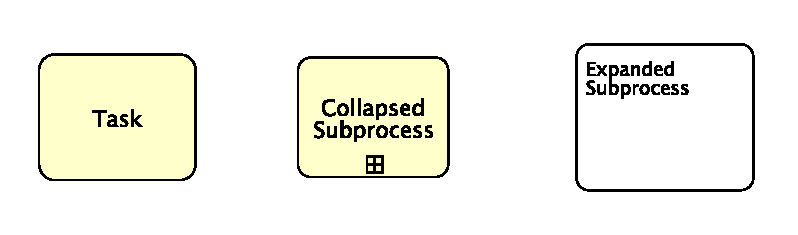
\includegraphics[width=0.5\textwidth]{images/processes.pdf}
\caption{BPMN activities: task, collapsed process, expanded subprocess}
\label{fig:task}
\end{figure}

\emph{Gateways} serve as means to control the flow of sequence in the diagram. As the term already implies, a gateway needs some ``mechanism that either allows or disallows passage through'' \citep{White:2004}. The result of a gateway pass-through can be that processes are merged or split. Graphically, a gateway is represented as a diamond. 

\begin{figure}[h]
\centering
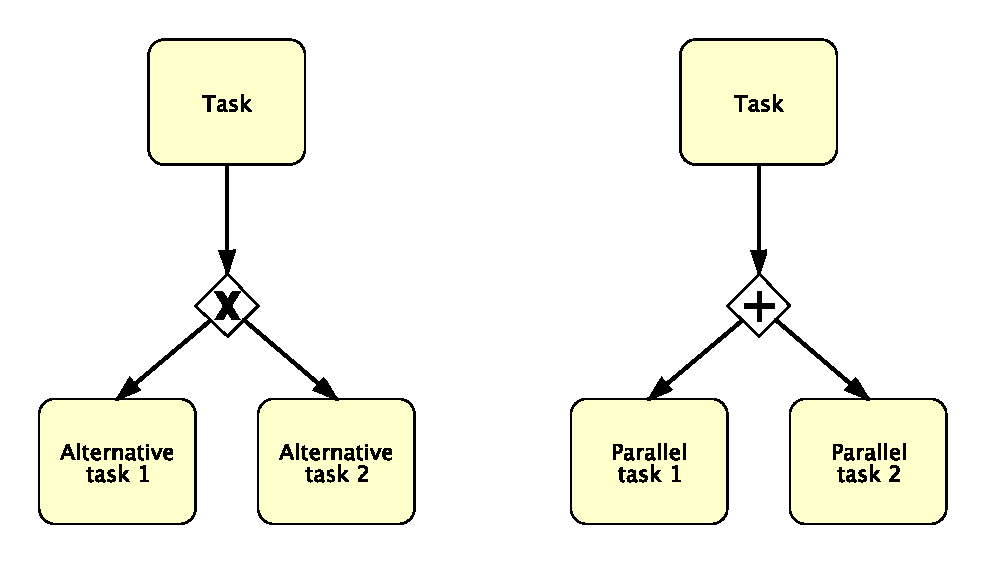
\includegraphics[width=0.5\textwidth]{images/gateways.pdf}
\caption{BPML gateway types: Exclusive (left), parallel (right)}
\label{fig:gateways}
\end{figure}

While there exist a number of different gateway types \citep[p.~93]{White:2004}, the SED-ML specification only uses the parallel and the exclusive gates  (\fig{gateways}). 

\emph{Exclusive} gateways -- also denoted as decisions -- allow the sequence flow to take two or more alternative paths (\fig{gateways}, left hand side). However, \emph{only one} of the paths may be chosen (not more). Sometimes two alternative branches need to be merged together again, in which case the exclusive gate must be used as well: The sequence flow continues as soon as \emph{one} of the incoming processes send a signal. An exclusive gateways is marked by an \code{X} in the graphical notation.

\emph{Parallel} gateways, ``provide a mechanism to synchronize parallel flow and to create parallel flow'' \citep{White:2004} (\fig{gateways}, right hand side). They are used to show parallel paths in the workflow; even if sometimes not required they might help in understanding the process. Synchronisation allows to start two processes in parallel at the same time in the sequence flow: The sequence flow will continue with \emph{all} processes leaving the parallel gateway. Joining two processes with a parallel gateway is also possible: the process flow will only continue after a signal has arrived from \emph{all} processes coming in the parallel gateway. A parallel gateway is marked by a \code{+} in the graphical notation.

\emph{Events} mark everything happening during the execution of the sequence flow, usually they interrrupt the business process, having some cause or impact on the execution. From the broad range of events that BPMN offers, SED-ML only uses a small subset, namely the start event and the end event (\fig{connectorEvents}).

\begin{figure}[h]
\centering
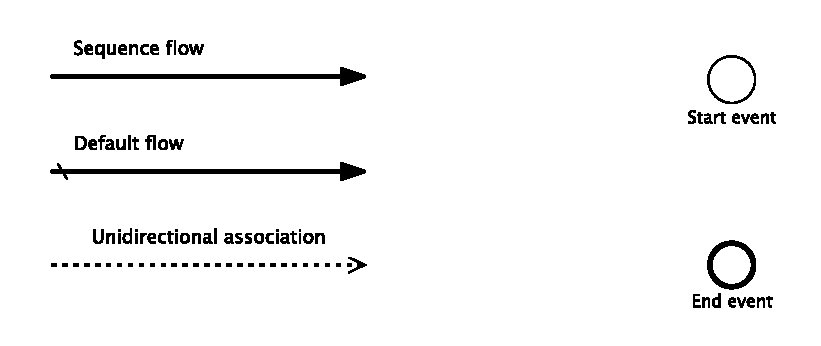
\includegraphics[width=0.5\textwidth]{images/connectors.pdf}
\caption{BPML connectors (left) and events (right).}
\label{fig:connectorEvents}
\end{figure}

All events are graphically drawn as small circles. A \emph{start event} is drawn with a single thin line and mark the start of a process, it can not have any incoming sequence flow. Start events may be triggered by different mechanisms, for the case of SED-ML the untyped start event (no marker inside the circle) is used. The trigger to start the process is ``Create new simulation experiment''. The \emph{end event} is marked with a thick line. It indicates the end of a process. SED-ML specification makes use of the untyped end event (no marker inside the circle). The end event is used to show the end of sub-processes as well as processes. If the end of a sub-process is reached, the sequence flow returns to the according parent process.

\emph{Connectors} are used to combine different BPMN objects with each other (\citet[p.~30]{White:2004} show the full list of valid connections). SED-ML uses only a subset of available connectors, namely sequence flow, default flow, and unidirectional associations (\fig{connectorEvents}). \emph{Sequence flow} defines the execution order of activities. \emph{Default flow} marks the default branch to be chosen if other conditions leave various possibilities for further execution of the sequence flow. A \emph{unidirectional association} is used to indicate that a data object is modified, i.\,e. read and written during the execution of an activity \citep{bpmnPoster}.

%
The rough SED-ML workflow is shown in Figure \ref{fig:sedmlWorkflow}.
%
\begin{figure}[h]
\centering
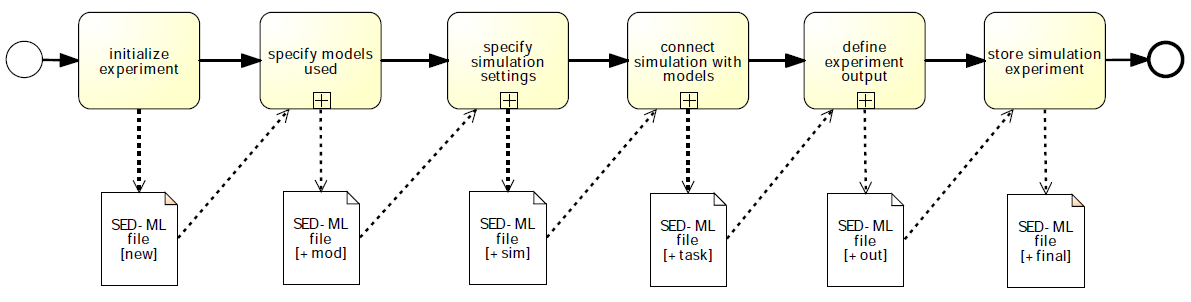
\includegraphics[width=\textwidth]{images/bpmn/sedMainOryx.png}
\caption{The process of defining a simulation experiment in SED-ML (overview)}
\label{fig:sedmlWorkflow}
\end{figure}
%
The process of defining a SED-ML simulation experiment starts by initialising the experiment and creating a new SED-ML file. Afterwards, the \concept{models} needed for the simulation are specified and stored into the existing SED-ML file (Section~\ref{overview:models}). In a third step, the simulation experiment \concept{setups} are defined and stored into the same file (Section~\ref{overview:simulation}). To assign a setup to a number of models used in the experiment, these connections have to be defined and recorded (Section~\ref{overview:task}), called \concept{task} in SED-ML. After simulation, the \concept{output} should be defined, based on the specified tasks and performed simulation experiment. The information is added to the existing SED-ML file (Section~\ref{overview:output}). In the end, the whole experiment is stored in the final SED-ML file.
%
All collapsed processes are described in the following sections. Examples in XML are provided in the more technical description.

\section{Models}
\label{overview:models}
To define a simulation experiment, first of all a new SED-ML file is created. The models to be used in the experiment (zero or many) are referenced, using a link to a model description in some open, curated model database (e.\,g.\ Biomodels Database \citep{LDR+10} or CellML Repository \citep{BBC+09}). All necessary changes to correctly simulate the model are defined, e.\,g., assigning new parameter values or updating the mathematics of the model (Figure~\ref{fig:workflowModel}).
%
\begin{figure}[h]
\centering
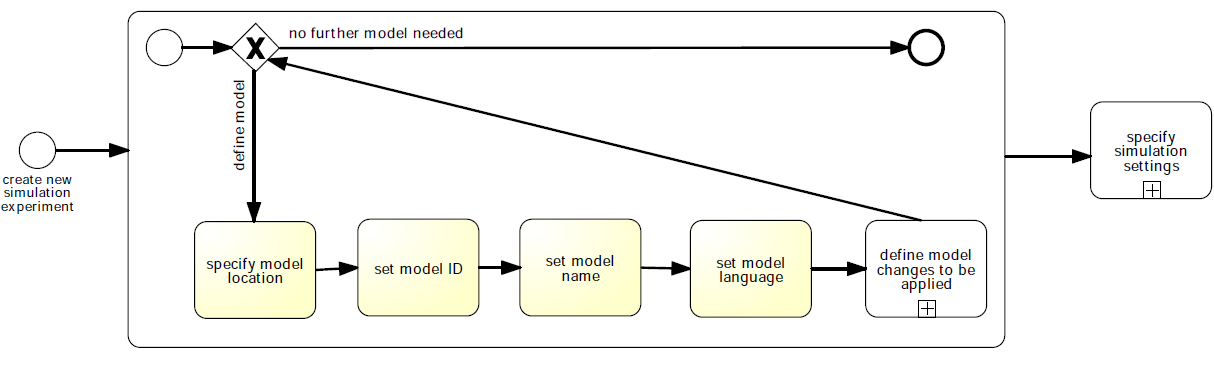
\includegraphics[width=0.8\textwidth]{images/bpmn/sedModelOryx.png}
\caption{The process of defining model(s) in SED-ML}
\label{fig:workflowModel}
\end{figure}
%
The procedure is repeated until all models participating in the experiment have been described. Each such model gets an internal SED-ML ID and an optional name.

\section{Simulation setup}
\label{overview:simulation}
Secondly, the simulation setups (zero or many) used throughout the simulation experiment are described (Figure \ref{fig:workflowSimulation}). 
%
%
\begin{figure}[h]
\centering
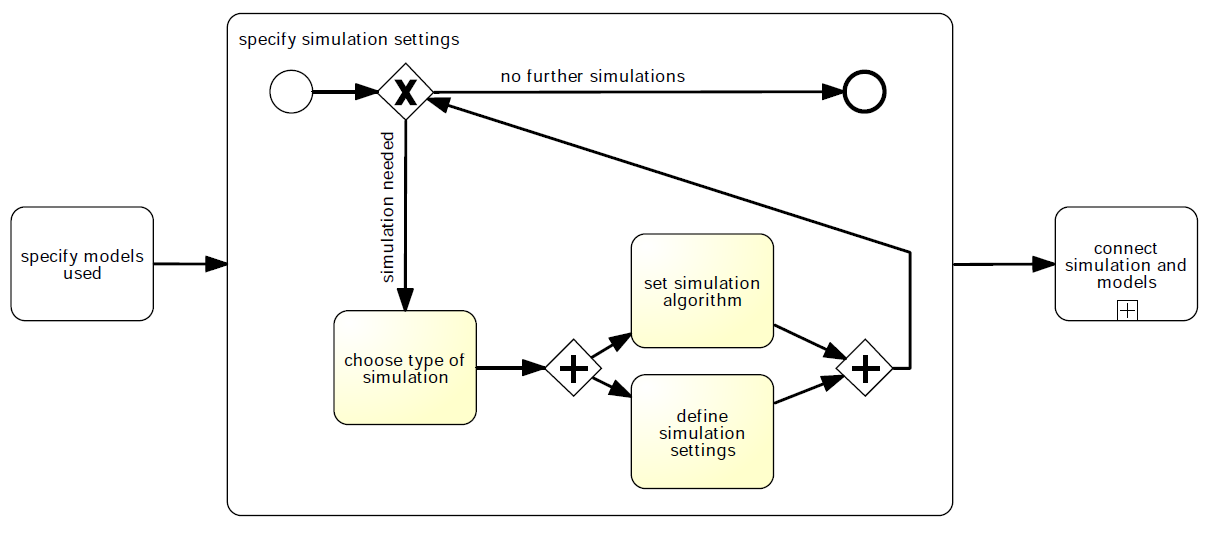
\includegraphics[width=0.8\textwidth]{images/bpmn/sedSimulationOryx.png}
\caption{The process of defining simulation(s) in SED-ML}
\label{fig:workflowSimulation}
\end{figure}
%
Those may stem from various different types of simulation, e.\,g., steady state analysis or bifurcation.  Depending on the specific type of experiment, the information encoded for the simulation setup might differ. Thus, the definition of simulation settings is specific to the simulation experiment.

In a simple case the experiment consists of one simulation, but it can get far more complex. For example, one might define a nested sequence of simulations, in which case every simulation has to be defined separately.
Each simulation setup gets its own internal ID and an optional name. For each of the setups, the simulation algorithm to be used for that simulation is defined through a reference to a well-defined algorithm name, e.\,g. an ontology or controlled vocabulary. One approach to define such a controlled vocabulary of simulation algorihtms is the \emph{Kinetic Simulation Algorithm Ontology} (Section~\ref{sec:kisao}). 
%
The setup definition is repeated until all different simulations have been described.

\section{Task}
\label{overview:task}
SED-ML allows to apply one defined simulation setting to one defined model at a time. However, any number of \concept{tasks} may be defined inside a simulation experiment description (Figure \ref{fig:workflowTask}). 
%
\begin{figure}[h]
\centering
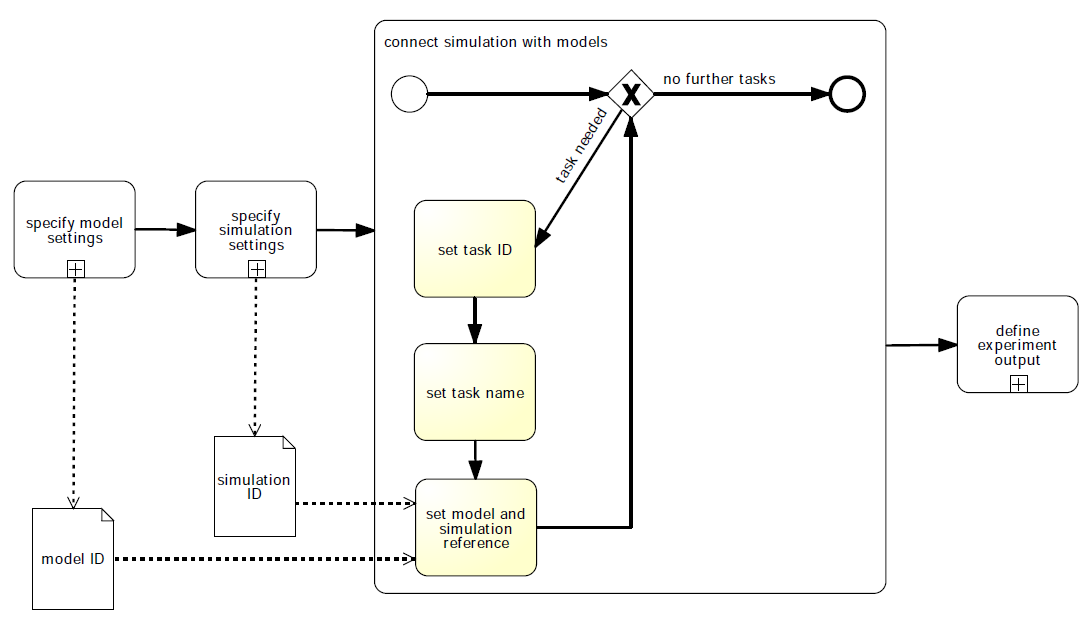
\includegraphics[width=0.7\textwidth]{images/bpmn/sedTaskOryx.png}
\caption{The process of defining simulation task(s) in SED-ML}
\label{fig:workflowTask}
\end{figure}
%
To do so, each task refers to one of the formerly specified models and to one of the formerly specified simulation setups. Each task has its own ID and an optional name. The process of task definition is repeated until all tasks have been defined.


\section{Output}
\label{overview:output}
The SED-ML finally consists of output definitions that describe what kind of output the experiment uses to present the simulation result to the user, i.\,e., a plot or a data table (Figure \ref{fig:workflowOutput}), and also which data is part of the output. 
%
\begin{figure}[h]
\centering
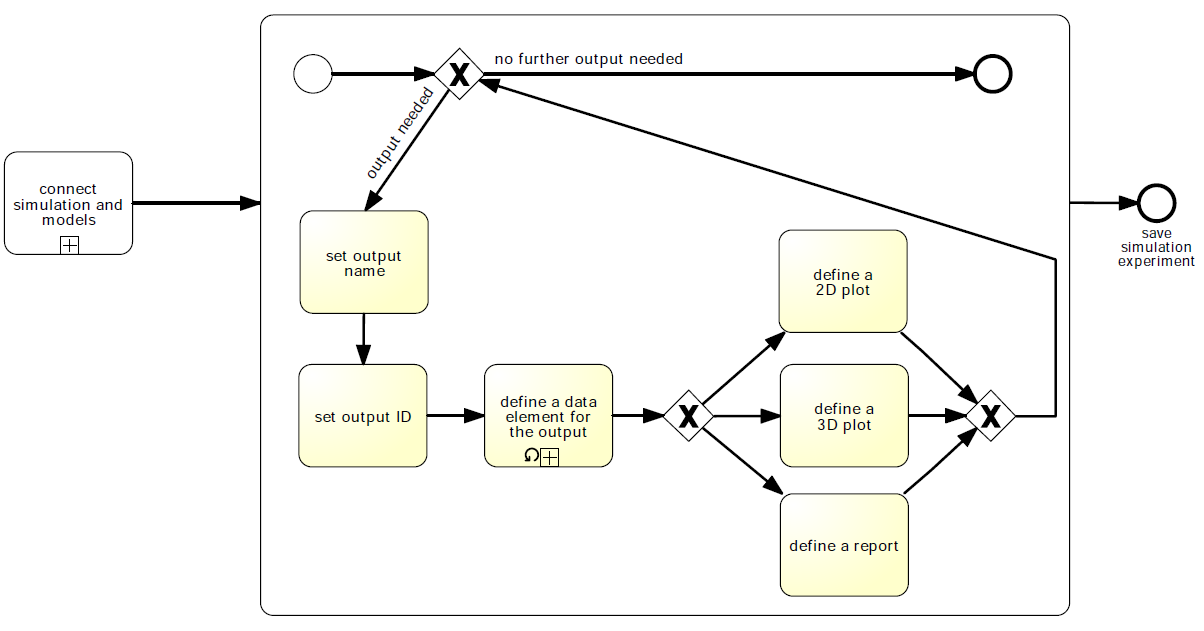
\includegraphics[width=0.7\textwidth]{images/bpmn/sedOutputOryx.png}
\caption{The process of defining output(s) in SED-ML}
\label{fig:workflowOutput}
\end{figure}
%
Therefore, SED-ML first defines a set of \concept{data generators} (Figure \ref{fig:workflowDataGenerator}), which are then used to specify a particular result, i.\,e. output (Section~\ref{overview:dataGen}). 

The SED-ML specification comes with three pre-defined types of outputs: 2D- and 3D plots, and reports. All use the aforementioned data generators to specify the information to be plotted on the different axes, or in the table comlumns respectively.
\section{Data Generator}
\label{overview:dataGen}
%
\begin{figure}[h]
\centering
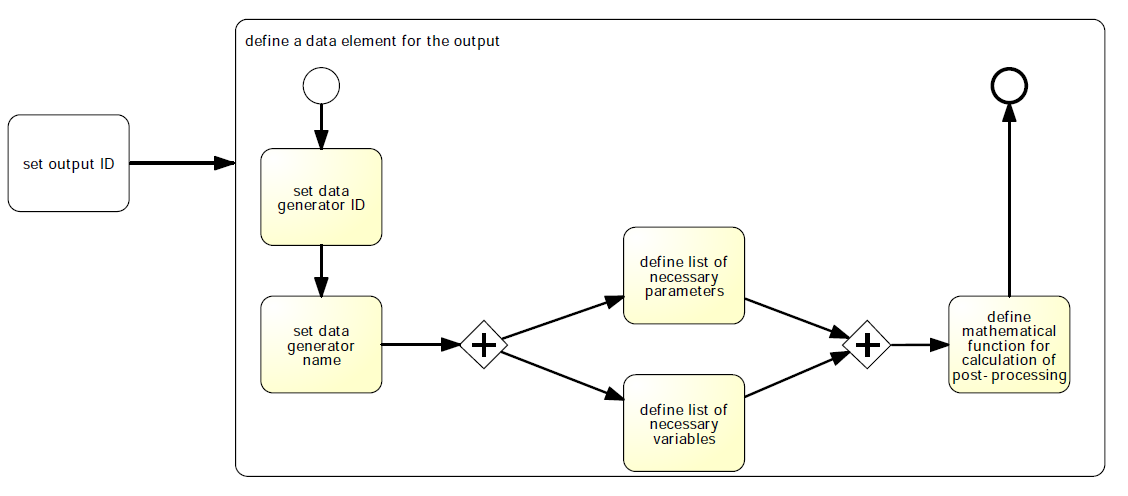
\includegraphics[width=0.7\textwidth]{images/bpmn/sedDataGeneratorOryx.png}
\caption{The process of defining data generator(s) in SED-ML}
\label{fig:workflowDataGenerator}
\end{figure}
%
A data generator may use data elements, e.\,g., variables or parameters, that either (1) have been taken directly from the model, or (2) have been generated in a post-processing step. If post-processing needs to be applied, variables and parameters from the various, previously defined models may be used, but also existing global parameters, such as \emph{time}.
If the variables are taken from existing models, a reference to the model and the particular variable needs to be given. 
If post-processing is necessary, a reference to an existing variable or parameter, including other data generators, has to be provided. Additional mathematical rules to be applied on the referred variable or parameter must then  be specified. 
%
In a SED-ML file, any number of data generators can be created for later re-use in the output definition.



%%% Local Variables: 
%%% mode: latex
%%% TeX-master: "../sed-ml-L1V2"
%%% End: 


%% XML SCHEMA
\section{XML Schema}
\label{sec:xmlschema}
Listing \ref{lst:schema} shows the full SED-ML XML Schema. The code is commented inline.
% SED-ML.xsd
\footnotesize
\begin{myXmlLst}{SED-ML XML Schema definition}{lst:schema}
<xs:schema targetNamespace="http://www.biomodels.net/sed-ml" xmlns="http://www.biomodels.net/sed-ml"
	xmlns:xs="http://www.w3.org/2001/XMLSchema" xmlns:math="http://www.w3.org/1998/Math/MathML">
	<xs:import namespace="http://www.w3.org/1998/Math/MathML"
		schemaLocation="sbml-mathml.xsd" />
		
<!-- global element declarations -->
	<xs:element name="variable">
		<xs:complexType>
			<xs:attribute name="taskReference" type="xs:string" use="optional" />
			<xs:attribute name="modelReference" type="xs:string" use="optional" />
			<xs:attribute name="name" type="xs:string" use="optional" />
			<!-- either target or symbol have to be used  in the variable definition-->
			<xs:attribute name="target" type="xs:token" use="optional" />
			<xs:attribute name="symbol" type="xs:string" use="optional" />
			<xs:attribute name="id" type="xs:string"/>
		</xs:complexType>
	</xs:element>
	<xs:element name="parameter">
		<xs:complexType>
		 	<xs:attribute name="id" type="xs:string" />
			<xs:attribute name="name" type="xs:string" use="optional" />
			<xs:attribute name="value" type="xs:double" use="required" />
		</xs:complexType>
	</xs:element>
	<xs:element name="algorithm">
		<xs:complexType>
			<xs:attribute name="kisaoID" type="xs:string" use="required"/>
		</xs:complexType>
	</xs:element>
	<xs:element name="uniformTimeCourse">
		<xs:complexType>
			<xs:sequence>
				<xs:element ref="algorithm"/>
			</xs:sequence>
			<xs:attribute name="id" type="xs:string" />
			<xs:attribute name="name" type="xs:string" use="optional" />
			<xs:attribute name="outputStartTime" type="xs:double"
				use="required" />
			<xs:attribute name="outputEndTime" type="xs:double" use="required" />
			<xs:attribute name="numberOfPoints" type="xs:integer"
				use="required" />
			<xs:attribute name="initialTime" type="xs:double" use="required" />
		</xs:complexType>
	</xs:element>
	<xs:element name="task">
		<xs:complexType>
			<xs:attribute name="simulationReference" type="xs:string"
				use="required" />
			<xs:attribute name="name" type="xs:string" use="optional" />
			<xs:attribute name="modelReference" type="xs:string"
				use="required" />
			<xs:attribute name="id" type="xs:string" />
		</xs:complexType>
	</xs:element>
	<xs:element name="notes" type="xs:string" />
	<xs:element name="annotation" type="xs:string" />
	<xs:complexType name="SEDBase">
		<xs:annotation>
			<xs:documentation xml:lang="en">
			The SEDBase type is the base type of all main types in SED-ML. It serves as a container for the annotation of any part of the experiment description.
		</xs:documentation>
		</xs:annotation>
		<xs:sequence>
			<xs:element ref="notes" minOccurs="0" />
			<xs:element ref="annotation" minOccurs="0" />
		</xs:sequence>
	</xs:complexType>
	<xs:element name="sedML">
		<xs:complexType>
			<xs:complexContent>
				<xs:extension base="SEDBase">
					<xs:sequence>
						<xs:element ref="listOfSimulations" />
						<xs:element ref="listOfModels" />
						<xs:element ref="listOfTasks" />
						<xs:element ref="listOfDataGenerators" />
						<xs:element ref="listOfOutputs" />
					</xs:sequence>
					<xs:attribute name="level " type="xs:decimal" use="required"
						fixed="1" />
					<xs:attribute name="version" type="xs:decimal" use="required"
						fixed="1" />
				</xs:extension>
			</xs:complexContent>
		</xs:complexType>
	</xs:element>
	<xs:element name="plot2D">
		<xs:complexType>
			<xs:sequence>
				<xs:element ref="listOfCurves" />
			</xs:sequence>
			<xs:attribute name="name" type="xs:string" use="optional" />
			<xs:attribute name="id" type="xs:string" />
		</xs:complexType>
	</xs:element>
	<xs:element name="plot3D">
		<xs:complexType>
			<xs:sequence>
				<xs:element ref="listOfSurfaces" />
			</xs:sequence>
			<xs:attribute name="name" type="xs:string" use="optional" />
			<xs:attribute name="id" type="xs:string" />
		</xs:complexType>
	</xs:element>
	<xs:element name="report">
		<xs:complexType>
			<xs:sequence>
				<xs:element ref="listOfDataSets" />
			</xs:sequence>
			<xs:attribute name="name" type="xs:string" use="optional" />
			<xs:attribute name="id" type="xs:string" />
		</xs:complexType>
	</xs:element>
	<xs:element name="model">
		<xs:complexType>
			<xs:sequence>
				<xs:element ref="listOfChanges" minOccurs="0" />
			</xs:sequence>
			<xs:attribute name="language" type="xs:anyURI" use="optional" default="urn:sedml:language:xml" />
			<xs:attribute name="source" type="xs:string" use="required"/>
			<xs:attribute name="name" type="xs:string" use="required" />
			<xs:attribute name="id" type="xs:string" use="required" />
		</xs:complexType>
	</xs:element>
	<xs:element name="math" type="math:Math" />
	<xs:element name="listOfVariables">
		<xs:complexType>
			<xs:sequence>
				<xs:element ref="variable" maxOccurs="unbounded" />
			</xs:sequence>
		</xs:complexType>
	</xs:element>
	<xs:element name="listOfParameters">
		<xs:complexType>
			<xs:sequence>
				<xs:element ref="parameter" maxOccurs="unbounded" />
			</xs:sequence>
		</xs:complexType>
	</xs:element>
	<xs:element name="listOfTasks">
		<xs:complexType>
			<xs:sequence>
				<xs:element ref="task" maxOccurs="unbounded" />
			</xs:sequence>
		</xs:complexType>
	</xs:element>
	<xs:element name="listOfSimulations">
		<xs:complexType>
			<xs:sequence>
				<xs:element ref="uniformTimeCourse" minOccurs="0" maxOccurs="unbounded"/>
			</xs:sequence>
		</xs:complexType>
	</xs:element>
	<xs:element name="listOfOutputs">
		<xs:complexType>
			<xs:sequence minOccurs="0">
				<xs:element ref="plot2D" minOccurs="0"  maxOccurs="unbounded"/>
				<xs:element ref="plot3D" minOccurs="0"  maxOccurs="unbounded"/>
				<xs:element ref="report" minOccurs="0"  maxOccurs="unbounded"/>
			</xs:sequence>
		</xs:complexType>
	</xs:element>
	<xs:element name="listOfModels">
		<xs:complexType>
			<xs:sequence>
				<xs:element ref="model" maxOccurs="unbounded" />
			</xs:sequence>
		</xs:complexType>
	</xs:element>
	<xs:element name="listOfDataGenerators">
		<xs:complexType>
			<xs:sequence>
				<xs:element ref="dataGenerator" maxOccurs="unbounded" />
			</xs:sequence>
		</xs:complexType>
	</xs:element>
	<xs:element name="listOfCurves">
		<xs:complexType>
			<xs:sequence>
				<xs:element ref="curve" maxOccurs="unbounded" />
			</xs:sequence>
		</xs:complexType>
	</xs:element>
	<xs:element name="listOfSurfaces">
		<xs:complexType>
			<xs:sequence>
				<xs:element ref="surface" maxOccurs="unbounded" />
			</xs:sequence>
		</xs:complexType>
	</xs:element>
	<xs:element name="listOfDataSets">
		<xs:complexType>
			<xs:sequence>
				<xs:element ref="dataSet" maxOccurs="unbounded" />
			</xs:sequence>
		</xs:complexType>
	</xs:element>
	<xs:element name="listOfChanges">
		<xs:complexType>
			<xs:sequence>
				<xs:element ref="changeAttribute" minOccurs="0"
					maxOccurs="unbounded" />
				<xs:element ref="changeXML" minOccurs="0" maxOccurs="unbounded" />
				<xs:element ref="computeChange" minOccurs="0" maxOccurs="unbounded" />
			</xs:sequence>
		</xs:complexType>
	</xs:element>
	<xs:element name="dataGenerator">
		<xs:complexType>
			<xs:sequence>
				<xs:element ref="listOfVariables" minOccurs="0" />
				<xs:element ref="listOfParameters" minOccurs="0" />
				<xs:element ref="math" />
			</xs:sequence>
			<xs:attribute name="name" type="xs:string" use="required" />
			<xs:attribute name="id" type="xs:string" />
		</xs:complexType>
	</xs:element>
	<xs:element name="curve">
		<xs:complexType>
		<xs:attribute name="id" use="required" type="xs:string" />
			<xs:attribute name="yDataReference" type="xs:string"
				use="required" />
			<xs:attribute name="xDataReference" type="xs:string"
				use="required" />
			<xs:attribute name="name" use="optional" type="xs:string" />
			<xs:attribute name="logY" use="required" type="xs:boolean" default="false"/>
			<xs:attribute name="logX" use="required" type="xs:boolean" default="false"/>
		</xs:complexType>
	</xs:element>
	<xs:element name="surface">
		<xs:complexType>
			<xs:attribute name="id" use="required" type="xs:string" />
			<xs:attribute name="yDataReference" type="xs:string"
				use="required" />
			<xs:attribute name="xDataReference" type="xs:string"
				use="required" />
			<xs:attribute name="zDataReference" type="xs:string"
				use="required" />
			<xs:attribute name="name" use="optional" type="xs:string" />
			<xs:attribute name="logY" use="required" type="xs:boolean" />
			<xs:attribute name="logX" use="required" type="xs:boolean" />
			<xs:attribute name="logZ" use="required" type="xs:boolean" />
		</xs:complexType>
	</xs:element>
	<xs:element name="dataSet">
		<xs:complexType>
			<xs:attribute name="id" use="required" type="xs:string" />
			<xs:attribute name="dataReference" type="xs:string" use="required"></xs:attribute>
			<xs:attribute name="label" use="required" type="xs:string" />
			<xs:attribute name="name" use="optional" type="xs:string" />
		</xs:complexType>
	</xs:element>
	<xs:element name="changeAttribute">
		<xs:complexType>
			<xs:attribute name="target" use="required" type="xs:token" />
			<xs:attribute name="newValue" type="xs:string" use="required" />
		</xs:complexType>
	</xs:element>
 	<xs:element name="newXML" type="xs:string" />
	<xs:element name="changeXML">
		<xs:complexType>
			<xs:sequence>
				<xs:element ref="newXML" />
			</xs:sequence>
			<xs:attribute name="target" use="required" type="xs:token" />
		</xs:complexType>
	</xs:element>	
	<xs:element name="computeChange">
		<xs:complexType>
			<xs:sequence>
				<xs:element ref="listOfVariables" />
				<xs:element ref="listOfParameters" />
				<xs:element ref="math" />
			</xs:sequence>
			<xs:attribute name="target" use="required" type="xs:token" />
		</xs:complexType>
	</xs:element>
</xs:schema>
\end{myXmlLst}

%%% Local Variables: 
%%% mode: latex
%%% TeX-master: "spec"
%%% End: 


%% SAMPLE FILE
\section{Examples}

\subsection{Le Loup Model (CellML)}
% sed-ml example file
The following example provides a SED-ML description for the simulation of the model based on the publication by Leoup, Gonze and Goldbeter ``Limit Cycle Models for Circadian Rhythms Based on Transcriptional Regulation in Drosophila and Neurospora'' (PubMed ID: 10643740).
The model source code is taken from the CellML Model Repository \citep{LLH+08}. 

The original model used in the simulation experiment is referred to using a URL (\url{http://models.cellml.org/workspace/leloup_gonze_goldbeter_1999/@@rawfile/d6613d7e1051b3eff2bb1d3d419a445bb8c754ad/leloup_gonze_goldbeter_1999_b.cellml}, ll. 14).
In order to set up the model some pre-processing needs to be applied: Those are defined in the \code{listOfChanges} from ll 15-23. All changes defined update particular parameter values in the model.

A second model is defined in l. 25 of the example, using \code{model1} as a source and applying even further changes to it, in this case updating two more model parameters.

One simulation setup is defined in the \code{listOfSimulations}. It is a \code{uniformTimeCourse} over 180 time units, using 1000 simulation points. The algorithm used is the CVODE solver, as denoted by the KiSAO ID \code{KiSAO:0000019}.

A number of \code{dataGenerator}s are defined in ll. 37-85. Those are the prerequisite for defining the output of the simulation. The first dataGenerator named \code{tim1} in l. 45 maps on the \code{Mt} entity in the model that is used in \code{task1} which here is the model with ID \code{model1}. The second dataGenerator named \code{per-tim} in l. 57 maps on the \code{CN} entity in \code{model1}. Finally  the third and fourth dataGenerators map on the \code{Mt} and \code{per-tim} entity respectively in the updated model with ID \code{model2}.

The \code{output} defined in the experiment consists of a 2D plot with two different curves (ll. 96-102). Both curves plot the \code{per-tim} concentration against the \code{tim} concentration. In the first curve the original parametrisation (as given in \code{model1}) is used, in the second curve the updated one is used (as given in \code{model2}).

\myXmlImport{LeLoup Model Simulation Description in SED-ML}{lst:leloup}{xml/leloupCellml.xml}

% \footnotesize
% \begin{myXmlLst}{LeLoup Model Simulation Description in SED-ML}{lst:leloup}
% <?xml version="1.0" encoding="utf-8"?>
% <sedML version="0.1" xmlns="http://www.biomodels.net/sed-ml" 
%        xmlns:math="http://www.w3.org/1998/Math/MathML">
%  <notes><p xmlns="http://www.w3.org/1999/xhtml">Comparing Limit Cycles and strange attractors for
%         oscillation in Drosophila</p></notes> 
%  <listOfSimulations>
%    <uniformTimeCourse id="simulation1" algorithm="KiSAO:0000019" 
%     initialTime="0" outputStartTime="0" outputEndTime="180" 
%     numberOfPoints="1000" >
%      <algorithm kisaoID="KISAO:0000019"/>
%     </uniformTimeCourse>
%  </listOfSimulations>
%  <listOfModels>
%   <model id="model1" name="Circadian Oscillations" language="urn:sedml:language:cellml" source="http://models.cellml.org/workspace/leloup_gonze_goldbeter_1999/@@rawfile/d6613d7e1051b3eff2bb1d3d419a445bb8c754ad/leloup_gonze_goldbeter_1999_a.cellml" >
%    <listOfChanges>
%     <changeAttribute target="/cellml:model/cellml:component[@cmeta:id='MP']/cellml:variable[@name='vsP']/@initial_value" newValue="1"/>
%     <changeAttribute target="/cellml:model/cellml:component[@cmeta:id='MP']/cellml:variable[@name='vmP']/@initial_value" newValue="0.7"/>
%     <changeAttribute target="/cellml:model/cellml:component[@cmeta:id='P2']/cellml:variable[@name='vdP']/@initial_value" newValue="2"/>
%     <changeAttribute target="/cellml:model/cellml:component[@cmeta:id='T2']/cellml:variable[@name='vdT']/@initial_value" newValue="2"/>  
%     <changeAttribute target="/cellml:model/cellml:component[@name='parameters']/cellml:variable[@name='k1']/@initial_value" newValue="0.6"/>
%     <changeAttribute target="/cellml:model/cellml:component[@name='parameters']/cellml:variable[@name='K4P']/@initial_value" newValue="1"/>
%     <changeAttribute target="/cellml:model/cellml:component[@name='parameters']/cellml:variable[@name='K4T']/@initial_value" newValue="1"/>
%    </listOfChanges>
%   </model>
%   <model id="model2" name="Circadian Chaos" language="urn:sedml:language:cellml" source="model1">
%    <listOfChanges>
%     <changeAttribute target="/cellml:model/cellml:component[@cmeta:id='MT']/cellml:variable[@name='vmT']/@initial_value" newValue="0.28"/>
%     <changeAttribute target="/cellml:model/cellml:component[@cmeta:id='T2']/cellml:variable[@name='vdT']/@initial_value" newValue="4.8"/>        
%    </listOfChanges>
%   </model>
%  </listOfModels>
 
%   <listOfTasks>
%     <task id="task1" name="Limit Cycle" modelReference="model1" simulationReference="simulation1"/>
%     <task id="task2" name="Strange attractors" modelReference="model2" simulationReference="simulation1"/>
%   </listOfTasks>
%   <listOfDataGenerators>
%     <dataGenerator id="tim1" name="tim mRNA">
%       <listOfVariables>
%         <variable id="v0" taskReference="task1" target="/cellml:model/cellml:component[@cmeta:id='MT']" />
%       </listOfVariables>
%        <math:math>
%           <math:apply>
%             <math:plus />
%             <math:ci>v0</math:ci>
%           </math:apply>
%         </math:math>
%     </dataGenerator>

%     <dataGenerator id="per-tim" name="nuclear PER-TIM complex">
%       <listOfVariables>
%         <variable id="v1" taskReference="task1" target="/cellml:model/cellml:component[@cmeta:id='CN']" />
%       </listOfVariables>
%       <math:math>
%         <math:apply>
%           <math:plus />
%           <math:ci>v1</math:ci>
%         </math:apply>
%       </math:math>
%     </dataGenerator>
    
%     <dataGenerator id="tim2" name="tim mRNA (changed parameters)">
%       <listOfVariables>
%         <variable id="v2" taskReference="task2" target="/cellml:model/cellml:component[@cmeta:id='MT']" />
%       </listOfVariables>  
%         <math:math>
%           <math:apply>
%             <math:plus />
%             <math:ci>v2</math:ci>
%           </math:apply>
%         </math:math>
%     </dataGenerator>
    
%     <dataGenerator id="per-tim2" name="nuclear PER-TIM complex">
%       <listOfVariables>
%         <variable id="v3" taskReference="task2" target="/cellml:model/cellml:component[@cmeta:id='CN']" />
%       </listOfVariables>
%       <math:math>
%         <math:apply>
%           <math:plus />
%           <math:ci>v3</math:ci>
%         </math:apply>
%       </math:math>
%     </dataGenerator>
%   </listOfDataGenerators>
  
%   <listOfOutputs>
%     <plot2D id="plot1" name="tim mRNA with Oscillation and Chaos">
%       <listOfCurves>
%         <curve id ="c1" logX="false" logY="false" xDataReference="per-tim" yDataReference="tim1" />
%         <curve id ="c2" logX="false" logY="false" xDataReference="per-tim2" yDataReference="tim2" />
%       </listOfCurves>
%     </plot2D>
%   </listOfOutputs>
% </sedML>
% \end{myXmlLst}



%%% Local Variables: 
%%% mode: latex
%%% TeX-master: "../sed-ml-L1V1"
%%% End: 


\end{appendix}

% REFERENCES
\bibliographystyle{plainnat}
\bibliography{sed-ml-L1V1}

\end{document}